%杨舒云的实验报告编辑界面,使用了Huanyu Shi,2019级的模板,杨舒云在此拜谢ORZ!

%!TEX program = xelatex
\documentclass[dvipsnames, svgnames,a4paper,11pt]{article}
% ----------------------------------------------------- 
%	加边框的命令
%	参考:https://tex.stackexchange.com/questions/531559/how-to-add-the-page-border-for-first-two-pages-in-latex
\usepackage{tikz}
\usetikzlibrary{calc}
\usepackage{eso-pic}
\AddToShipoutPictureBG{%
\begin{tikzpicture}[overlay,remember picture]
\draw[line width=0.6pt] % 边框粗细
    ($ (current page.north west) + (0.6cm,-0.6cm) $)
    rectangle
    ($ (current page.south east) + (-0.6cm,0.6cm) $); % 边框位置
\end{tikzpicture}}


\usepackage{xcolor}
\definecolor{c1}{HTML}{086173} % 目录颜色 原版为2752C9 紫灰色535AAA 蓝紫色0B0DB7 深蓝色070F94 湖绿色219394 松石灰绿086173
\definecolor{c2}{HTML}{E20129} % 引用颜色 原版\definecolor{c2}{RGB}{190,20,83} 橙色F24729

\usepackage{ctex}
\usepackage[top=28mm,bottom=28mm,left=15mm,right=15mm]{geometry}
\usepackage{hyperref} 
\hypersetup{
	colorlinks,
	linktoc = section, % 超链接位置,选项有section, page, all
	linkcolor = c1, % linkcolor 目录颜色
	citecolor = c1  % citecolor 引用颜色
}
\usepackage{amsmath,enumerate,multirow,float}
\usepackage{tabularx}
\usepackage{tabu}
\usepackage{subfig}
\usepackage{fancyhdr}
\usepackage{graphicx}
\usepackage{wrapfig}  
\usepackage{physics}
\usepackage{appendix}
\usepackage{amsfonts}

%
\usepackage{tcolorbox}
\tcbuselibrary{skins,breakable}
\newtcolorbox{tbox}[2][]{
    colframe=black!70!,
    breakable,
    enhanced,
	boxrule =0.5pt,
    title = {#2},
    fonttitle = \large\kaishu\bfseries,
	drop fuzzy shadow,
    #1
}
\newtcolorbox[auto counter,number within=section]{question}[1][]{
  top=2pt,bottom=2pt,arc=1mm,
  boxrule=0.5pt,
%   frame hidden,
  breakable,
  enhanced, %跨页后不会显示下边框
  coltitle=c1!80!gray,
  colframe=c1,
  colback=c1!3!white,
  drop fuzzy shadow,
  title={思考题~\thetcbcounter:\quad},
  fonttitle=\bfseries,
  attach title to upper,
  #1
}

% ---------------------------------------------------------------------
%	利用cleveref改变引用格式,\cref是引用命令
\usepackage{cleveref}
\crefformat{figure}{#2{\textcolor{c2}{Figure #1}}#3} % 图片的引用格式
\crefformat{equation}{#2{(\textcolor{c2}{#1})}#3} % 公式的引用格式
\crefformat{table}{#2{\textcolor{c2}{Table #1}}#3} % 表格的引用格式


% ---------------------------------------------------------------------
%	页眉页脚设置
\fancypagestyle{plain}{\pagestyle{fancy}}
\pagestyle{fancy}
\lhead{\kaishu 中山大学物理与天文学院电子技术实验\uppercase\expandafter{\romannumeral1}} % 左边页眉,学院 + 课程
\rhead{\kaishu 实验报告By杨舒云\&戴鹏辉} % 右边页眉,实验报告标题
\cfoot{\thepage} % 页脚,中间添加页码


% ---------------------------------------------------------------------
%	对目录、章节标题的设置
\renewcommand{\contentsname}{\centerline{\huge 目录}}
\usepackage{titlesec}
\usepackage{titletoc}
% \titleformat{章节}[形状]{格式}{标题序号}{序号与标题间距}{标题前命令}[标题后命令]
\titleformat{\section}{\centering\LARGE\songti}{}{1em}{}

% ---------------------------------------------------------------------
%   listing代码环境设置
\usepackage{listings}
\lstloadlanguages{python}
\lstdefinestyle{pythonstyle}{
backgroundcolor=\color{gray!5},
language=python,
frameround=tftt,
frame=shadowbox, 
keepspaces=true,
breaklines,
columns=spaceflexible,                   
basicstyle=\ttfamily\small, % 基本文本设置,字体为teletype,大小为scriptsize
keywordstyle=[1]\color{c1}\bfseries, 
keywordstyle=[2]\color{Red!70!black},   
stringstyle=\color{Purple},       
showstringspaces=false,
commentstyle=\ttfamily\scriptsize\color{green!40!black},%注释文本设置,字体为sf,大小为smaller
tabsize=2,
morekeywords={as},
morekeywords=[2]{np, plt, sp},
numbers=left, % 代码行数
numberstyle=\it\tiny\color{gray}, % 代码行数的数字字体设置
stepnumber=1,
rulesepcolor=\color{gray!30!white}
}




% ---------------------------------------------------------------------
%	其他设置
\def\degree{${}^{\circ}$} % 角度
\graphicspath{{./images/}} % 插入图片的相对路径
\allowdisplaybreaks[4]  %允许公式跨页 
\usepackage{lipsum}
\usepackage{adjustbox}
\usepackage{booktabs}
\usepackage{multicol}

%\usepackage{mathrsfs} % 字体
\captionsetup[figure]{name=Figure} % 图片形式
\captionsetup[table]{name=Table} % 表格形式

\begin{document}
	
	
	
	% 实验报告封面	
	
	% 顶栏
	\begin{table}
		\renewcommand\arraystretch{1.7}
		\begin{tabularx}{\textwidth}{
				|X|X|X|X
				|X|X|X|X|}
			\hline
			\multicolumn{2}{|c|}{预习报告}&\multicolumn{2}{|c|}{实验记录}&\multicolumn{2}{|c|}{分析讨论}&\multicolumn{2}{|c|}{总成绩}\\
			\hline
			\LARGE 25 & & \LARGE25 & & \LARGE30 & & \LARGE80 & \\
			\hline
		\end{tabularx}
	\end{table}
	% ---
	
	% 信息栏
	\begin{table}
		\renewcommand\arraystretch{1.7}
		\begin{tabularx}{\textwidth}{|X|X|X|X|}
			\hline
			年级、专业: & 2022级 物理学 &组号: & 实验组E2\\
			\hline
			姓名: & 戴鹏辉、杨舒云  & 学号: & 22344016、223444020\\
			\hline
			实验时间: & 2024/03/04 & 教师签名: & \\
			\hline
		\end{tabularx}
	\end{table}
	% ---
	
	% 大标题
	\begin{center}
		\LARGE 实验二 \quad 基本电路元件伏安特性的测量
	\end{center}
	% ---
	
	% 注意事项
	
	% 基本
	\textbf{【实验报告注意事项】}
	\begin{enumerate}
		\item 实验报告由三部分组成:
		\begin{enumerate}
			\item 预习报告:课前认真研读实验讲义,弄清实验原理;实验所需的仪器设备、用具及其使用、完成课前预习思考题;了解实验需要测量的物理量,并根据要求提前准备实验记录表格(可以参考实验报告模板,可以打印)。\textcolor{red}{\textbf{(20分)}}
			\item 实验记录:认真、客观记录实验条件、实验过程中的现象以及数据。实验记录请用珠笔或者钢笔书写并签名(\textcolor{red}{\textbf{用铅笔记录的被认为无效}})。\textcolor{red}{\textbf{保持原始记录,包括写错删除部分,如因误记需要修改记录,必须按规范修改。}}(不得输入电脑打印,但可扫描手记后打印扫描件);离开前请实验教师检查记录并签名。\textcolor{red}{\textbf{(30分)}}
			\item 数据处理及分析讨论:处理实验原始数据(学习仪器使用类型的实验除外),对数据的可靠性和合理性进行分析;按规范呈现数据和结果(图、表),包括数据、图表按顺序编号及其引用;分析物理现象(含回答实验思考题,写出问题思考过程,必要时按规范引用数据);最后得出结论。\textcolor{red}{\textbf{(30分)}}
		\end{enumerate}
		\textbf{实验报告就是将预习报告、实验记录、和数据处理与分析合起来,加上本页封面。\textcolor{red}{(80分)}}
		\item 每次完成实验后的一周内交\textbf{实验报告}(特殊情况不能超过两周)。
		\item \textbf{其它注意事项}:
		\begin{enumerate}
			\item 请认真查看并理解实验讲义第一章内容;
			\item 注意实验器材的合理使用;
			\item 使用结束使用各种仪器之后需要将其放回原位。
		\end{enumerate}
	\end{enumerate}
	
	% 安全
%	\textbf{【实验安全注意事项】}	
%	\begin{enumerate}
%		\item 
%	\end{enumerate}
	
	% ---
	
%	% 特别鸣谢
%	\textbf{【特别鸣谢及模板说明】}	
%	
%	感谢2019级学长石寰宇为本实验报告提供\LaTeX 模板。\textcolor{red}{\textbf{由于原实验报告模板缺少实验编号,为方便在电脑上整理,故添加自命名编号}}
%	% ---
	
	
	
	% 目录
	\clearpage
	\tableofcontents
	\clearpage
	% ---
	
	
	
	% 预习报告	
	
	% 小标题
	\setcounter{section}{0}
	\section{实验二\quad 基本电路元件伏安特性的测量 \quad\heiti 预习报告}
	% ---
	
	% 实验目的
	\subsection{实验目的}
	\begin{enumerate}
		\item 学习基本电路元件伏安特性的测试方法。
		
		\item 进一步练习直流稳压电源、万用表的使用方法。
		
	\end{enumerate}
	% ---
	
	% 仪器用具
	\subsection{仪器用具}
	\begin{table}[htbp]
		\centering
		\renewcommand\arraystretch{1.6}
		% \setlength{\tabcolsep}{10mm}
		\begin{tabular}{p{0.05\textwidth}|p{0.20\textwidth}|p{0.05\textwidth}|p{0.5\textwidth}}
			\hline
			编号& 仪器用具名称 & 数量 &  主要参数(型号,测量范围,测量精度等) \\
			\hline
			1 & 电路原理实验箱 & 1 & {\footnotesize《元件伏安特性的研究》单元和《受控源1、受控源2》单元}  \\
			\hline
			2 & 线性电阻元件   & 2 & $R_1=10K·120\Omega$ \quad $R_2=51\Omega$ \\
			\hline
			3 & 非线性电阻元件 & 1 & 12V白炽灯 \\
			\hline
			4 & 电位器$R_w$ & 1 & 可接成固定电阻、可调电阻和分压器三种形式 \\
			\hline
			5 & 直流稳压电源  & 1 &  \\
			\hline
			6 & 直流电流表、电压表  & 1 &  \\
			\hline
			7 & 直流电压表  & 1 &  \\
			\hline
			8 & 电流表专用线及实验导线  & 若干 &  \\
			\hline
		\end{tabular}
	\end{table}
	% ---
	
	% 原理概述
	\subsection{原理概述}
	\begin{enumerate}
		\item \textbf{伏安特性}:也称为电压-电流特性,是描述电路元件在不同电压作用下电流变化规律的一种特性。它反映了元件两端电压与通过元件的电流之间的关系。可以通过绘制伏安特性曲线来直观表示,其中横轴通常是电压(V),纵轴是电流(I)。
		
		如\cref{fig:fig1}所示,电路的基本元件主要包括电阻器、电容器、电感器和二极管等。每种元件的伏安特性(即电压-电流关系)都有其特点:
		
		\begin{itemize}
			\item 电阻器:遵循欧姆定律,电流与电压成正比,其比例系数即为电阻值。伏安关系线性,通过原点。
			\item 电容器:电流与电压变化率成正比,关系式为 \(I = C \frac{dV}{dt}\),其中 \(C\) 是电容值。伏安曲线表现为电压变化时电流的峰值。
			\item 电感器:电流的变化率与电压成正比,关系式为 \(V = L \frac{dI}{dt}\),其中 \(L\) 是电感值。伏安特性显示在电流变化时电压的峰值。
			\item 二极管:具有非线性伏安特性,只有当电压超过一定阈值时电流才显著增加,显示出单向导电的性质。
		\end{itemize}
		
		
		\begin{figure}[htbp]
			\centering
			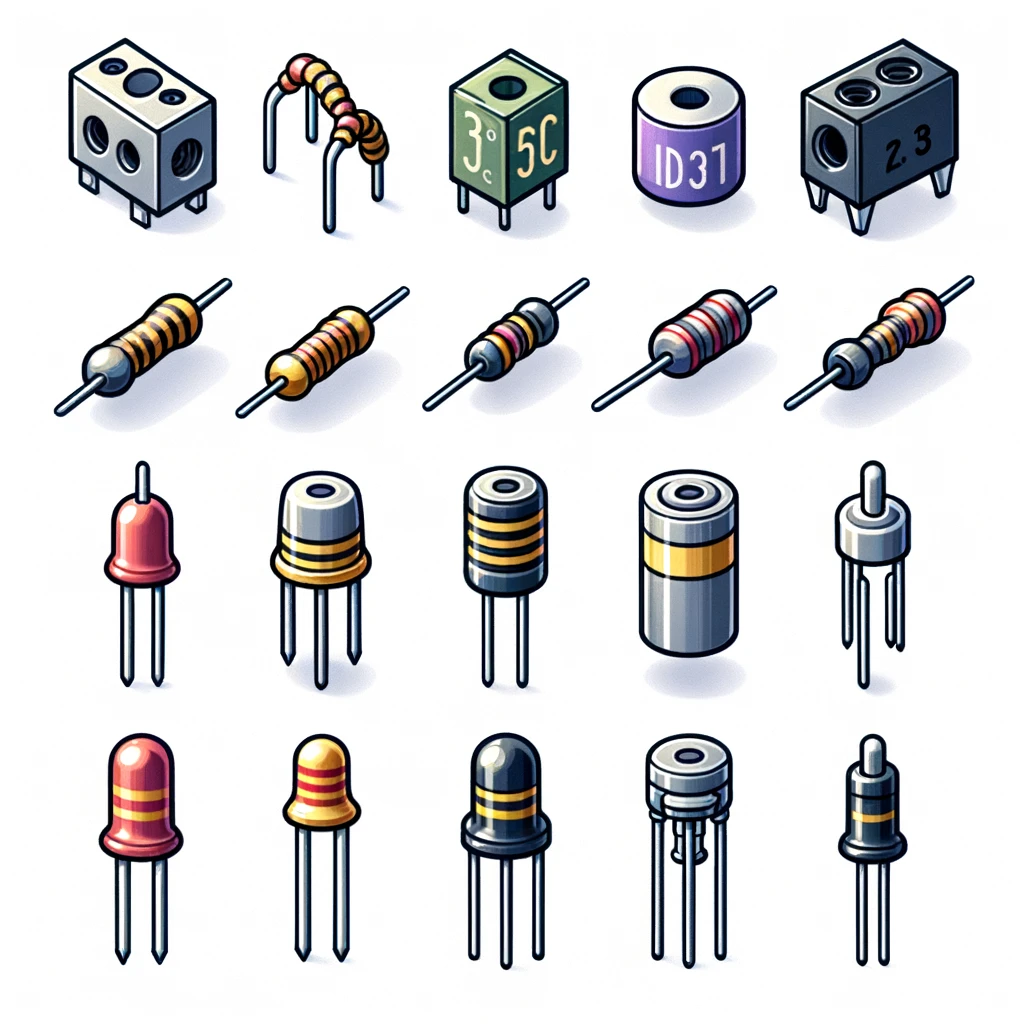
\includegraphics[width=0.3\textwidth]{ET1_2Gra1.png}
			\caption{一些元件}
			\label{fig:fig1}
		\end{figure}
		
		如果将电阻元件的电压视为横坐标,电流视为纵坐标,绘制电压与电流的关系曲线,这条曲线称为该元件的伏安特性。
		
		\item \textbf{线性元件的伏安特性}:线性电阻元件的伏安特性在\(V-I\)(或\(I-V\))平面上是通过坐标原点的直线,与元件电压或电流的方向无关,是双向性的元件,最典型的线性元件是电阻器;其关系遵从欧姆定律,电阻值可由以下公式确定:\[R = \frac{V}{I}\]
		$R$表示电阻阻值,$V$表示电阻两端电压以及$I$表示流经电阻电流。
		
		\item \textbf{考虑发热对电阻伏安特性的影响}:电阻在通电时会发热,称为焦耳热。电阻的温度升高会导致其电阻值变化(对于金属电阻,温度上升,电阻值增加;对于半导体材料,温度上升,电阻值减少)。这种现象会影响电阻的伏安特性,使得原本线性的关系出现偏差。
		
		\item \textbf{常见非线性元件的伏安特性}:
		\begin{itemize}
			\item 电流控制型电阻元件:如果元件的端电压是流过该元件电流的单值函数,则称为电流控制型电阻元件。这类元件的电阻值随着通过它的电流的变化而变化,如NTC(负温度系数)热敏电阻,其电阻随温度(进而是电流)的增加而减小。
			\item 电压控制型的电阻元件:如果通过元件的电流是该元件端电压的单值函数,则称为电压控制型的电阻元件。这类元件的电阻值随着两端电压的变化而变化,如VDR(电压依赖性电阻器),其电阻随电压的增加而减小。
			\item 既是电流控制型又是电压控制型的电阻元件:如果元件的伏安特性曲线是单调增加或减少的,则该元件同时具有电流控制型和电压控制型的特性。某些特殊电阻元件可能同时受电流和电压的控制,如MEMS(微电子机械系统)技术中的某些传感器。
		\end{itemize}
		
		\begin{figure}[htbp]
			\centering
			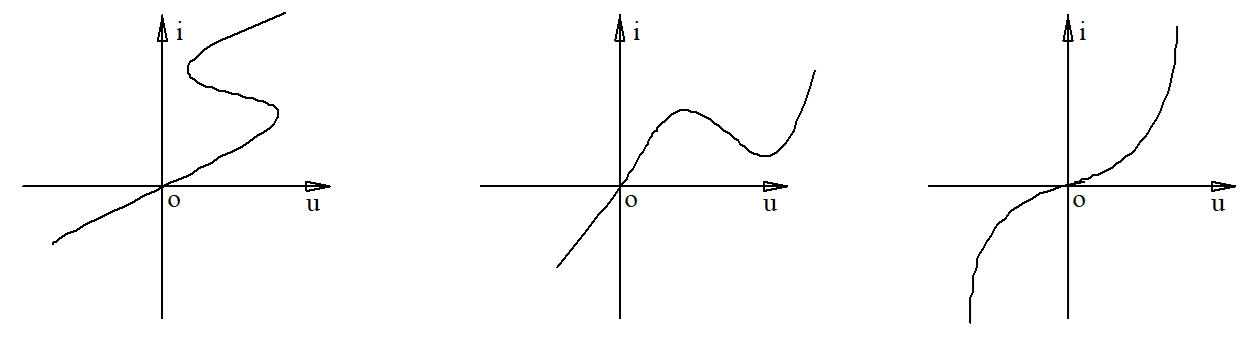
\includegraphics[width=0.9 \textwidth]{ET1_2Gra3.png}
			\caption{非线性电阻元件的伏安特性示意图}
			\label{fig:fig3}
		\end{figure}
		
		\item \textbf{受控源}:
		\begin{itemize}
			\item 什么是受控源:受控源分为独立源(如电池和发电机)和非独立源(也称受控源),受控源的输出电压或电流随网络中某支路的电压或电流变化而变化。
			\item 四种理想受控源的转移特性表示:
			\begin{enumerate}
				\item 电压控制电压源(VCVS):输出电压与输入电压成比例,转移电压比为\(\mu\), 表示为$U_2 = \mu U_1$。
				\item 电流控制电压源(CCVS):输出电压与输入电流成比例,转移电阻为\(\gamma\), 表示为$U_2 = \gamma I_1$。
				\item 电压控制电流源(VCCS):输出电流与输入电压成比例,转移电导为\(\gamma\), 表示为$I_2 = gU_1$。
				\item 电流控制电流源(CCCS):输出电流与输入电流成比例,转移电流比为\(\beta\), 表示为$I_2 = \beta I_1$。
			\end{enumerate}
		\end{itemize}
	\end{enumerate}

		\begin{figure}[htbp]
			\centering
			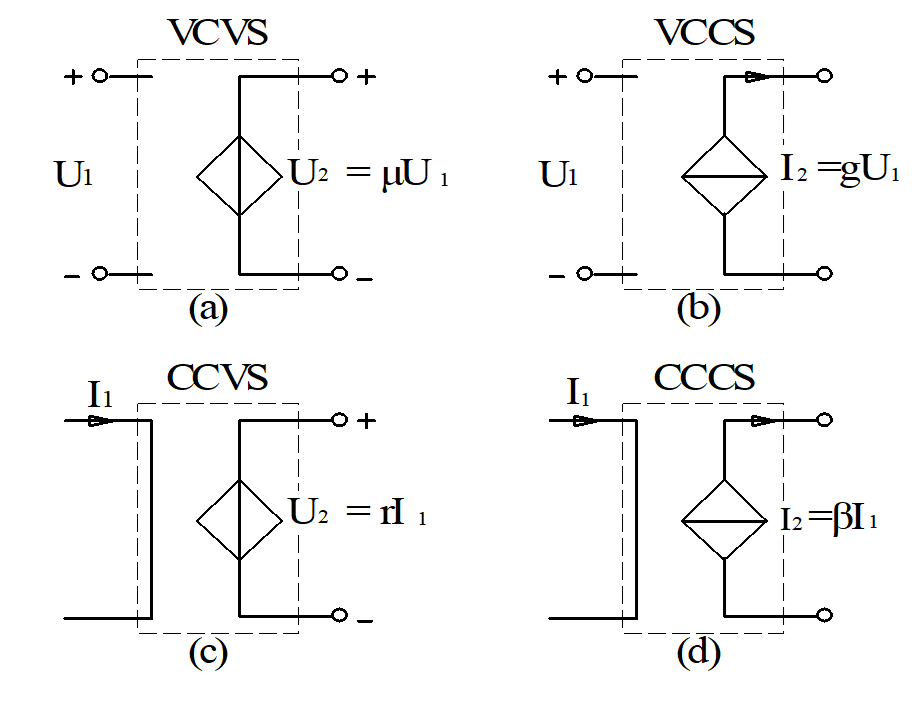
\includegraphics[width=0.5\textwidth]{ET1_2Gra4.png}
			\caption{四种理想受控源}
			\label{fig:fig4}
		\end{figure}


	% ---
	
	
	
	% 实验前思考题
	\subsection{实验预习题}
	
	% 思考题1
	\begin{question}
		预习了解电路基本元件及其伏安特性;考虑发热对电阻伏安特性的影响。
	\end{question}
	见\textbf{原理概述}部分。
	
	% 思考题2
	\begin{question}
		万用表电压档与电流档的内阻范围以及内阻对测量的影响
	\end{question}
	\begin{itemize}
		\item 电压档:万用表在测量电压时具有较高的内阻(通常在 \(M\Omega\) 级别),以减小对电路的影响。
		\item 电流档:万用表在测量电流时的内阻相对较低,为了减少测量过程中的电压降。
		\item 万用表的内阻对测量结果有一定的影响。高内阻有助于电压测量时减少对电路的加载,而低内阻有助于电流测量时减小电压降,从而提高测量准确度。
	\end{itemize}
	
	% 思考题3
	\begin{question}
		受控源和独立源相比有何异同点?比较两种受控源的代号、控制量与被控制量的关系如何?
	\end{question}
	独立源与受控源:
	\begin{itemize}
		\item 独立源:其输出不依赖于电路中其他元件的电压或电流。分为电压源和电流源。
		\item 受控源:输出依赖于电路中某些其他元件的电压或电流。分为电压控制电压源(VCVS)、电流控制电压源(CCVS)、电压控制电流源(VCCS)和电流控制电流源(CCCS)。
	\end{itemize}
	
	受控源的代号及其控制量与被控制量的关系:
	\begin{itemize}
		\item VCVS:电压控制电压源,输出电压与输入电压成正比。
		\item CCVS:电流控制电压源,输出电压与输入电流成正比。
		\item VCCS:电压控制电流源,输出电流与输入电压成正比。
		\item CCCS:电流控制电流源,输出电流与输入电流成正比。
	\end{itemize}
	
	详见\textbf{原理概述}部分。
	
	\begin{question}
		两种受控源中的g、$\gamma$的意义是什么?如何测得?
	\end{question}
	在受控源中,“g”通常表示电压控制电流源(VCCS)的转移系数,即输出电流与输入电压的比例系数。而“$\gamma$”表示电流控制电压源(CCVS)的转移系数,即输出电压与输入电流的比例系数。
	
	这些转移系数可以通过实验测定,即通过改变输入量(电压或电流),观察输出量的变化,从而计算得到。
	
	\begin{question}
		受控源输入输出是否符合能量守恒,其中的能量转移是怎么进行的?
	\end{question}
	受控源在理想情况下是符合能量守恒原则的,但它们不是能量的独立来源。受控源的输出能量来自于电路的其他部分或外部供电。在实际电路中,受控源模拟的是通过其他电路元件(如放大器)对输入信号进行放大或转换的过程,这个过程中能量的来源是这些元件的供电,而不是受控源本身。因此,受控源的能量转移实际上是通过电路中的能量转换和放大来实现的,遵循能量守恒定律。
	
	% ---
	
	
	
	% 实验记录	
	\clearpage
	
	% 顶栏
	\begin{table}
		\renewcommand\arraystretch{1.7}
		\centering
		\begin{tabularx}{\textwidth}{|X|X|X|X|}
			\hline
			专业: & 物理学 & 年级: & 2022级 \\
			\hline
			姓名: & 戴鹏辉、杨舒云 & 学号: & 22344016、22344020\\
			\hline
			室温: & 20\degree C & 实验地点: & A522 \\
			\hline
			学生签名:& 见\textbf{附件}部分 & 评分: &\\
			\hline
			实验时间:& 2024/3/4 & 教师签名:&\\
			\hline
		\end{tabularx}
	\end{table}
	% ---
	
	% 小标题
	\section{实验二\quad 基本电路元件伏安特性的测量  \quad\heiti 实验记录}
	% ---
	
	% 实验过程记录
	\subsection{实验内容、步骤与结果}
	
	%
	\subsubsection{操作步骤记录}
	\begin{enumerate}
		
		\item 测试线性电阻元件的伏安特性

			\begin{figure}[htbp]
				\centering
				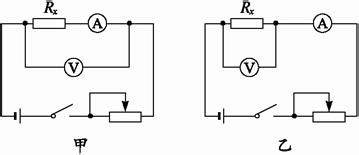
\includegraphics[width=0.5\textwidth]{ET1_2GraVA0.jpg}
				\caption{内外接法电路图}
				\label{fig:figdata-0}
			\end{figure}

		\begin{enumerate}
			\item 用电压表和电流表分别采用方法一(电压表外接 法)和方法二(电流表外接法)的两种接线方法进行测试,比较测试结果。
			\item 阈值设置:通过计算得到,当电阻两端功率不超过1W时,最大电压和电流分别为:
			\begin{itemize}
				\item $51\Omega$:$I_{max}=0.14A$,$U_{max}=7.14V$;
				\item $120\Omega$:$I_{max}=0.09A$,$U_{max}=10.95V$;
			\end{itemize}
			\item 测试目的:观察外接法和内接法的测量效果哪一个更显著。
			\item 线性电阻元件的伏安特性测量,分别采用方法一和方法二,电路如图所示。电压表可不用固定接在电路中,电压表两端接专用带测试表笔的导线,测量时直接用测试表笔插到测试点既可。
			\item 计算电阻值,是根据测量的电压、电流值进行计算,结果记入自拟表格中即可。
		\end{enumerate}
		
		\item 测试非线性电阻 12V 白炽灯的伏安特性,测试电路参考线性电阻。
		
			\begin{figure}[htbp]
				\centering
				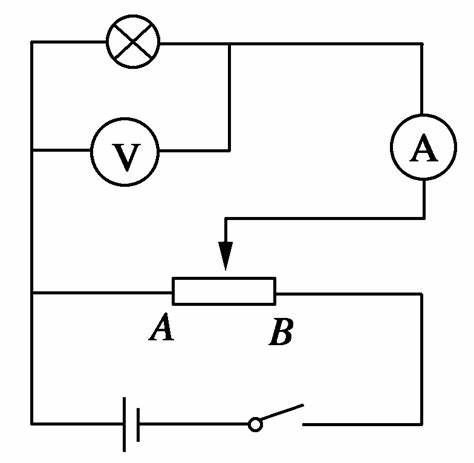
\includegraphics[width=0.3\textwidth]{ET1_2GraVA4.jpg}
				\caption{小灯泡伏安特性电路图}
				\label{fig:figdata-4-1}
			\end{figure}

		\begin{enumerate}
			\item 阈值设置:最大电压不能超过 12V,防止功率过大,烧坏元件。小灯泡在模拟电路实验箱中。
			\item 电路图如\cref{fig:figdata-4-1}所示。
		\end{enumerate}
		
		\item 测试直流稳压电源(DP832 或 DP831)CH2 的伏安特性,设定电压 6.0V,限流 20mA,自行设计测试电路。
		
			\begin{figure}[htbp]
				\centering
				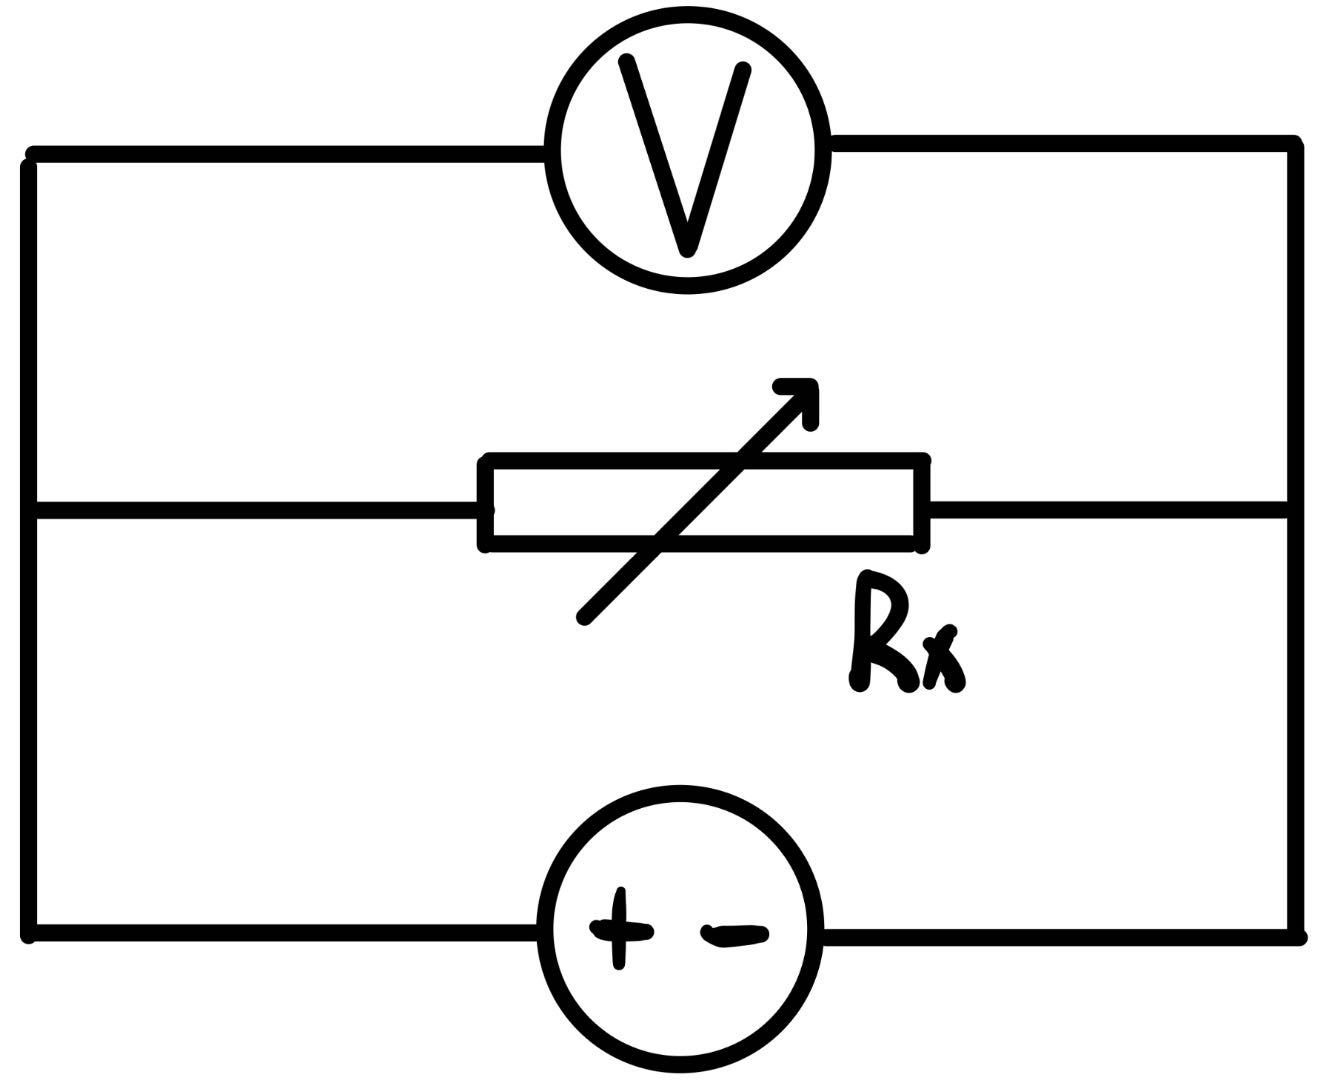
\includegraphics[width=0.3\textwidth]{ET1_2GraVA5.jpg}
				\caption{测试直流稳压电源伏安特性电路图}
				\label{fig:figdata-5}
			\end{figure}

		\begin{enumerate}
			\item 测量原理:利用电压表测电阻两端电压,也是源两端电压;
			然后利用电压除以电阻箱已知电阻计算电流,从而完成对伏安特性的测量。
			\item 电路图如\cref{fig:figdata-5}所示。
			\item 阈值设置:$I_{max}=0.02A$。
		\end{enumerate}
		
		\item 测试数控恒流源(DCS-01)的伏安特性,设定电流 1mA,自行设计测试电路。
		
			\begin{figure}[htbp]
				\centering
				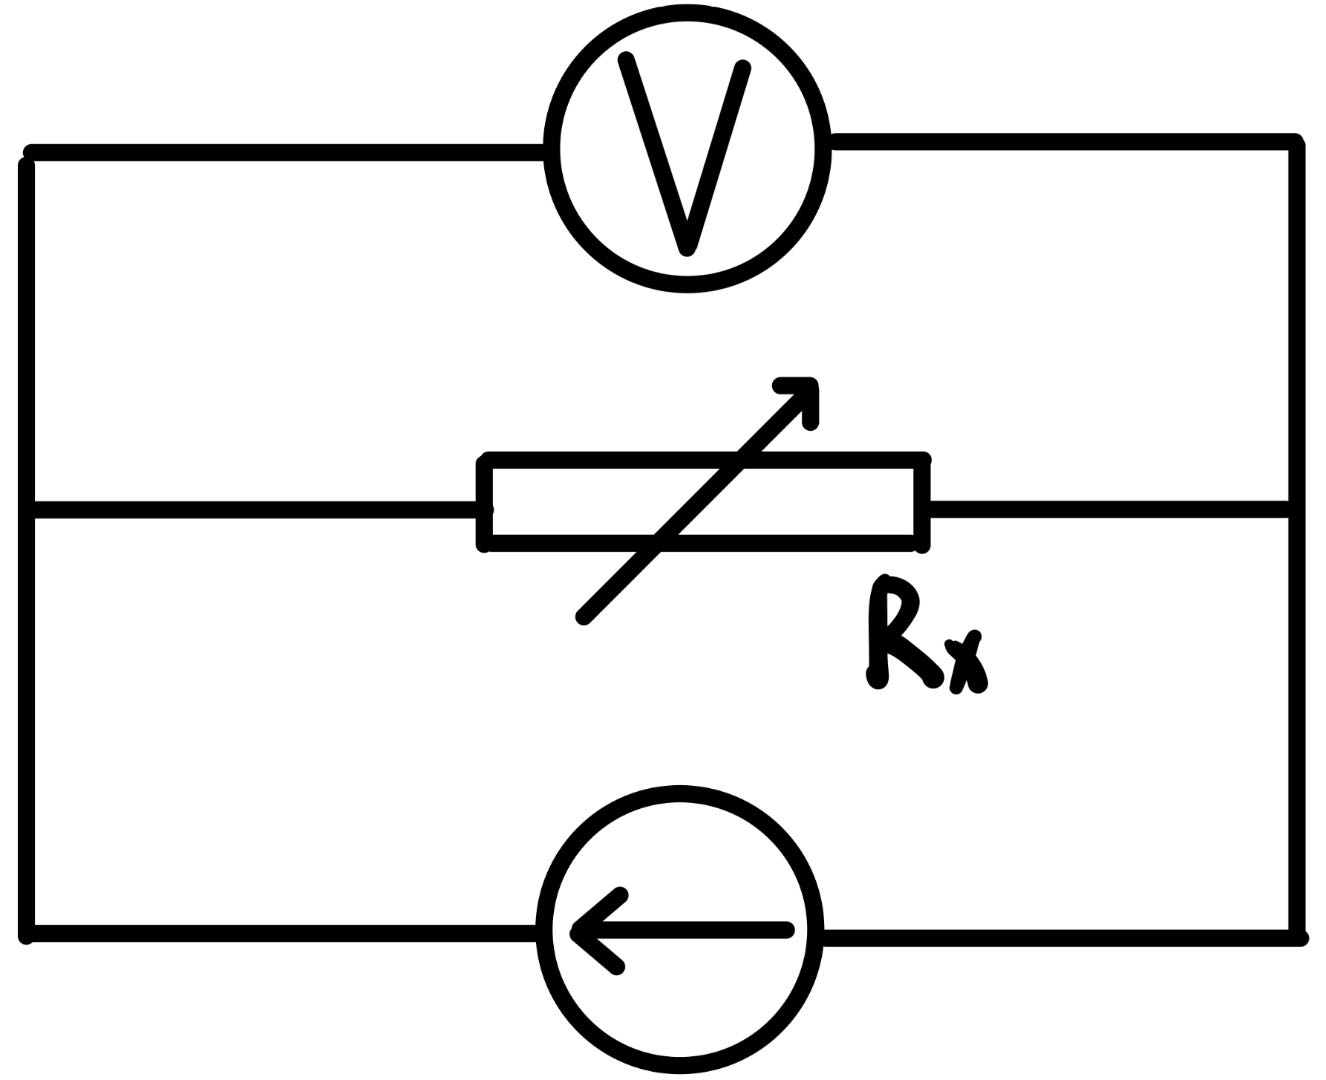
\includegraphics[width=0.3\textwidth]{ET1_2GraVA6.jpg}
				\caption{测试数控恒流源伏安特性电路图}
				\label{fig:figdata-6}
			\end{figure}

		\begin{enumerate}
			\item 测量原理:利用电压表测电阻两端电压,也是源两端电压;
			然后利用电压除以电阻箱已知电阻计算电流,从而完成对伏安特性的测量。
			\item 电路图如\cref{fig:figdata-6}所示。
			\item 阈值设置:$U_{max}=13.7V$。
		\end{enumerate}
		
		\item 电流控制电压源(CCVS)基本特性测试
		\begin{enumerate}
		\item 首先,我们先测量了它的\textbf{转移特性},这可以帮助我们判断它是否能正常工作。
		
		使 CCVS 负载 \(RL = 2K\Omega\),改变控制量 \(I_1\) 大小,用万用表测量输出电压 \(U_2\),记录数据。
				
		\item 接着,我们进一步测量了\textbf{输出特性}。
		
		使 CCVS 控制电流 \(I_1=100\mu A\)(不能超过 \(1mA\)),负载电阻分别为 \(1K\Omega\)、\(3K\Omega\)、\(5K\Omega\) 时,用万用表测量输出电压 \(U_2\) 和输出电流 \(I_2\),将数据填入表中。
		\end{enumerate}
	\end{enumerate}	
	
	%
	\subsubsection{实验数据记录}
	\begin{enumerate}
		\item 测试线性电阻元件的伏安特性
		
		\begin{table}[htbp]
			\centering
			\caption{数据:线性电阻元件的伏安特性(51$\Omega$)}
			\begin{tabular}{|c|c|c|c|}
				\hline
				\multicolumn{2}{|c|}{51Ω 外接} & \multicolumn{2}{c|}{51Ω 内接} \\
				\hline
				电压/V & 电流/mA & 电压/V & 电流/mA \\
				\hline
				0.964 & 18.900 & 0.994 & 18.900 \\
				1.929 & 37.830 & 1.988 & 37.780 \\
				2.894 & 56.800 & 2.983 & 55.900 \\
				3.856 & 75.740 & 3.977 & 75.860 \\
				4.820 & 95.200 & 4.970 & 95.500 \\
				5.780 & 113.800 & 5.960 & 114.700 \\
				6.740 & 133.700 & 6.960 & 134.300 \\
				\hline
			\end{tabular}%
			\label{tab:tab1}%
		\end{table}%
		
		\begin{table}[htbp]
			\centering
			\caption{数据:线性电阻元件的伏安特性(120$\Omega$)}
			\begin{tabular}{|c|c|c|c|}
				\hline
				\multicolumn{2}{|c|}{120Ω 外接} & \multicolumn{2}{c|}{120Ω 内接} \\
				\hline
				电压/V & 电流/mA & 电压/V & 电流/mA \\
				\hline
				0.982 & 8.210 & 0.995 & 8.210 \\
				1.963 & 16.420 & 1.990 & 16.420 \\
				2.945 & 24.640 & 2.985 & 24.650 \\
				3.925 & 32.870 & 3.981 & 32.890 \\
				4.910 & 41.120 & 4.980 & 41.170 \\
				5.890 & 49.400 & 5.970 & 49.480 \\
				6.870 & 57.700 & 6.960 & 57.820 \\
				7.850 & 66.180 & 7.960 & 66.250 \\
				8.840 & 74.700 & 8.960 & 74.790 \\
				9.820 & 83.200 & 9.950 & 83.300 \\
				\hline
			\end{tabular}%
			\label{tab:tab2}%
		\end{table}%
		
		实验数据如\cref{tab:tab1}和\cref{tab:tab2}所示。
		
		\item 测试非线性电阻 12V 白炽灯的伏安特性
		
		% \begin{table}[htbp]
		% 	\centering
		% 	\caption{数据:12V白炽灯的伏安特性}
		% 	\label{tab:tab3}
		% 	\begin{tabular}{|c|c|c|}
		% 		\hline
		% 		电压/V & 电流/mA & 电阻R/Ω \\
		% 		\hline
		% 		0.879 & 24.1 & 36.47 \\
		% 		1.834 & 29.9 & 61.34 \\
		% 		2.777 & 35.4 & 78.45 \\
		% 		3.680 & 40.4 & 91.09 \\
		% 		4.630 & 45.5 & 101.76 \\
		% 		5.600 & 50.4 & 111.11 \\
		% 		6.550 & 55.3 & 118.44 \\
		% 		7.570 & 59.4 & 127.44 \\
		% 		8.550 & 64.0 & 133.59 \\
		% 		9.540 & 68.2 & 139.88 \\
		% 		10.560 & 71.6 & 147.49 \\
		% 		11.520 & 75.5 & 152.58 \\
		% 		\hline
		% 	\end{tabular}
		% \end{table}

		\begin{table}[htbp]
			\centering
			\caption{数据:12V白炽灯的伏安特性}
			\label{tab:tab3}
			\small
			\begin{tabular}{|c|c|c|c|c|c|c|c|c|c|c|c|c|}
				\hline
				电压/V & 0.879 & 1.834 & 2.777 & 3.680 & 4.630 & 5.600 & 6.550 & 7.570 & 8.550 & 9.540 & 10.560 & 11.520 \\
				\hline
				电流/mA & 24.1 & 29.9 & 35.4 & 40.4 & 45.5 & 50.4 & 55.3 & 59.4 & 64.0 & 68.2 & 71.6 & 75.5 \\
				\hline
				电阻R/Ω & 36.47 & 61.34 & 78.45 & 91.09 & 101.76 & 111.11 & 118.44 & 127.44 & 133.59 & 139.88 & 147.49 & 152.58 \\
				\hline
			\end{tabular}
		\end{table}
		
		实验数据如\cref{tab:tab3}所示。
		
		\item 测试直流稳压电源(DP832 或 DP831)CH2 的伏安特性
		
		% \begin{table}[htbp]
		% 	\centering
		% 	\caption{数据:直流稳压电源的伏安特性}
		% 	\label{tab:tab4}
		% 	\begin{tabular}{|c|c|c|}
		% 		\hline
		% 		Rx/Ω & U/V & Ix/A \\
		% 		\hline
		% 		60 & 1.240 & 0.0207 \\
		% 		90 & 1.857 & 0.0206 \\
		% 		100 & 2.064 & 0.0206 \\
		% 		200 & 4.126 & 0.0206 \\
		% 		300 & 5.996 & 0.0200 \\
		% 		400 & 5.996 & 0.0150 \\
		% 		500 & 5.996 & 0.0120 \\
		% 		600 & 5.997 & 0.0100 \\
		% 		700 & 5.997 & 0.0086 \\
		% 		800 & 5.997 & 0.0075 \\
		% 		900 & 5.998 & 0.0067 \\
		% 		1000 & 5.998 & 0.0060 \\
		% 		2000 & 5.998 & 0.0030 \\
		% 		3000 & 5.998 & 0.0020 \\
		% 		6000 & 5.998 & 0.0010 \\
		% 		9000 & 5.998 & 0.0007 \\
		% 		\hline
		% 	\end{tabular}
		% \end{table}

		\begin{table}[htbp]
			\centering
			\begin{minipage}{.5\linewidth}
			  \centering
			  \caption{数据:直流稳压电源的伏安特性}
				\begin{tabular}{|c|c|c|}
					\hline
					Rx/Ω & U/V & Ix/A \\
					\hline
					60 & 1.240 & 0.0207 \\
					90 & 1.857 & 0.0206 \\
					100 & 2.064 & 0.0206 \\
					200 & 4.126 & 0.0206 \\
					300 & 5.996 & 0.0200 \\
					400 & 5.996 & 0.0150 \\
					500 & 5.996 & 0.0120 \\
					600 & 5.997 & 0.0100 \\
					700 & 5.997 & 0.0086 \\
					800 & 5.997 & 0.0075 \\
					900 & 5.998 & 0.0067 \\
					1000 & 5.998 & 0.0060 \\
					2000 & 5.998 & 0.0030 \\
					3000 & 5.998 & 0.0020 \\
					6000 & 5.998 & 0.0010 \\
					9000 & 5.998 & 0.0007 \\
					\hline
				\end{tabular}
			  \label{tab:tab4}
			\end{minipage}%
			\begin{minipage}{.5\linewidth}
			  \centering
			  \caption{数据:数控恒流源的伏安特性}
			  \begin{tabular}{|c|c|c|}
				\hline
				Rx/Ω & U/mV & Ix/mA \\
				\hline
				0.1 & 0.12 & 1.21 \\
				0.2 & 0.23 & 1.14 \\
				0.3 & 0.33 & 1.11 \\
				1 & 1.06 & 1.06 \\
				2 & 2.11 & 1.05 \\
				3 & 3.15 & 1.05 \\
				10 & 10.47 & 1.05 \\
				20 & 20.93 & 1.05 \\
				30 & 31.37 & 1.05 \\
				100 & 104.39 & 1.04 \\
				200 & 209.00 & 1.05 \\
				300 & 313.00 & 1.04 \\
				1000 & 1043.00 & 1.04 \\
				2000 & 2086.00 & 1.04 \\
				3000 & 3130.00 & 1.04 \\
				10000 & 10407.00 & 1.04 \\
				8500 & 8850.00 & 1.04 \\
				8600 & 8950.00 & 1.04 \\
				11000 & 11442.00 & 1.04 \\
				12000 & 12480.00 & 1.04 \\
				13000 & 13527.00 & 1.04 \\
				14000 & 13580.00 & 0.97 \\
				15000 & 13588.00 & 0.91 \\
				16000 & 13600.00 & 0.85 \\
				\hline
			\end{tabular}
			  \label{tab:tab5}
			\end{minipage}
			
			
		\end{table}

		
		实验数据如\cref{tab:tab4}所示。
		
		\item 测试数控恒流源(DCS-01)的伏安特性
		
		% \begin{table}[h]
		% 	\centering
		% 	\caption{数据:数控恒流源的伏安特性}
		% 	\label{tab:tab5}
		% 	\begin{tabular}{|c|c|c|}
		% 		\hline
		% 		Rx/Ω & U/mV & Ix/mA \\
		% 		\hline
		% 		0.1 & 0.12 & 1.21 \\
		% 		0.2 & 0.23 & 1.14 \\
		% 		0.3 & 0.33 & 1.11 \\
		% 		1 & 1.06 & 1.06 \\
		% 		2 & 2.11 & 1.05 \\
		% 		3 & 3.15 & 1.05 \\
		% 		10 & 10.47 & 1.05 \\
		% 		20 & 20.93 & 1.05 \\
		% 		30 & 31.37 & 1.05 \\
		% 		100 & 104.39 & 1.04 \\
		% 		200 & 209.00 & 1.05 \\
		% 		300 & 313.00 & 1.04 \\
		% 		1000 & 1043.00 & 1.04 \\
		% 		2000 & 2086.00 & 1.04 \\
		% 		3000 & 3130.00 & 1.04 \\
		% 		10000 & 10407.00 & 1.04 \\
		% 		8500 & 8850.00 & 1.04 \\
		% 		8600 & 8950.00 & 1.04 \\
		% 		11000 & 11442.00 & 1.04 \\
		% 		12000 & 12480.00 & 1.04 \\
		% 		13000 & 13527.00 & 1.04 \\
		% 		14000 & 13580.00 & 0.97 \\
		% 		15000 & 13588.00 & 0.91 \\
		% 		16000 & 13600.00 & 0.85 \\
		% 		\hline
		% 	\end{tabular}
		% \end{table}
		
		实验数据如\cref{tab:tab5}所示。
		
		\item 电流控制电压源(CCVS)基本特性测试
		
		转移特性实验数据如\cref{tab:tabA1}所示。
		
		% \begin{table}[htbp]
		% 	\centering
		% 	\caption{数据:CCVS转移特性}
		% 	\label{tab:tabA1}
		% 	\begin{tabular}{|c|c|}
		% 		\hline
		% 		I1/mA & U2/V \\
		% 		\hline
		% 		100.000 & 0.198 \\
		% 		120.131 & 0.236 \\
		% 		140.115 & 0.277 \\
		% 		159.982 & 0.316 \\
		% 		180.042 & 0.355 \\
		% 		199.977 & 0.395 \\
		% 		\hline
		% 	\end{tabular}
		% \end{table}		
		
		输出特性实验数据如\cref{tab:tabA2}所示。
		
		% \begin{table}[htbp]
		% 	\centering
		% 	\caption{数据:CCVS输出特性}
		% 	\label{tab:tabA2}
		% 	\begin{tabular}{|c|c|c|}
		% 		\hline
		% 		R/KΩ & I2/mA & U2/V \\
		% 		\hline
		% 		1 & 101.668 & 0.101 \\
		% 		2 & 100.046 & 0.196 \\
		% 		3 & 98.439 & 0.291 \\
		% 		4 & 96.888 & 0.383 \\
		% 		5 & 95.384 & 0.472 \\
		% 		\hline
		% 	\end{tabular}
		% \end{table}	

		\begin{table}[htbp]
			\centering
			\begin{minipage}{.5\linewidth}
			  \centering
			  \caption{数据:CCVS转移特性}
			  \begin{tabular}{|c|c|}
				\hline
				I1/mA & U2/V \\
				\hline
				100.000 & 0.198 \\
				120.131 & 0.236 \\
				140.115 & 0.277 \\
				159.982 & 0.316 \\
				180.042 & 0.355 \\
				199.977 & 0.395 \\
				\hline
			\end{tabular}
			  \label{tab:tabA1}
			\end{minipage}%
			\begin{minipage}{.5\linewidth}
			  \centering
			  \caption{数据:CCVS输出特性}
			  \begin{tabular}{|c|c|c|}
				\hline
				R/KΩ & I2/mA & U2/V \\
				\hline
				1 & 101.668 & 0.101 \\
				2 & 100.046 & 0.196 \\
				3 & 98.439 & 0.291 \\
				4 & 96.888 & 0.383 \\
				5 & 95.384 & 0.472 \\
				\hline
			\end{tabular}
			  \label{tab:tabA2}
			\end{minipage}
			
			
		\end{table}

		
	\end{enumerate}	
	% ---
	
	% 原始数据
	\clearpage
	\subsection{原始数据记录}
	实验记录本上的原始数据见\cref{fig:figdata-1}、\cref{fig:figdata-2}、\cref{fig:figdata-3}和\cref{fig:figdata-4}(签字)。
	
	\begin{figure}[htbp]
		\centering
		\subfloat[原始数据1]
		{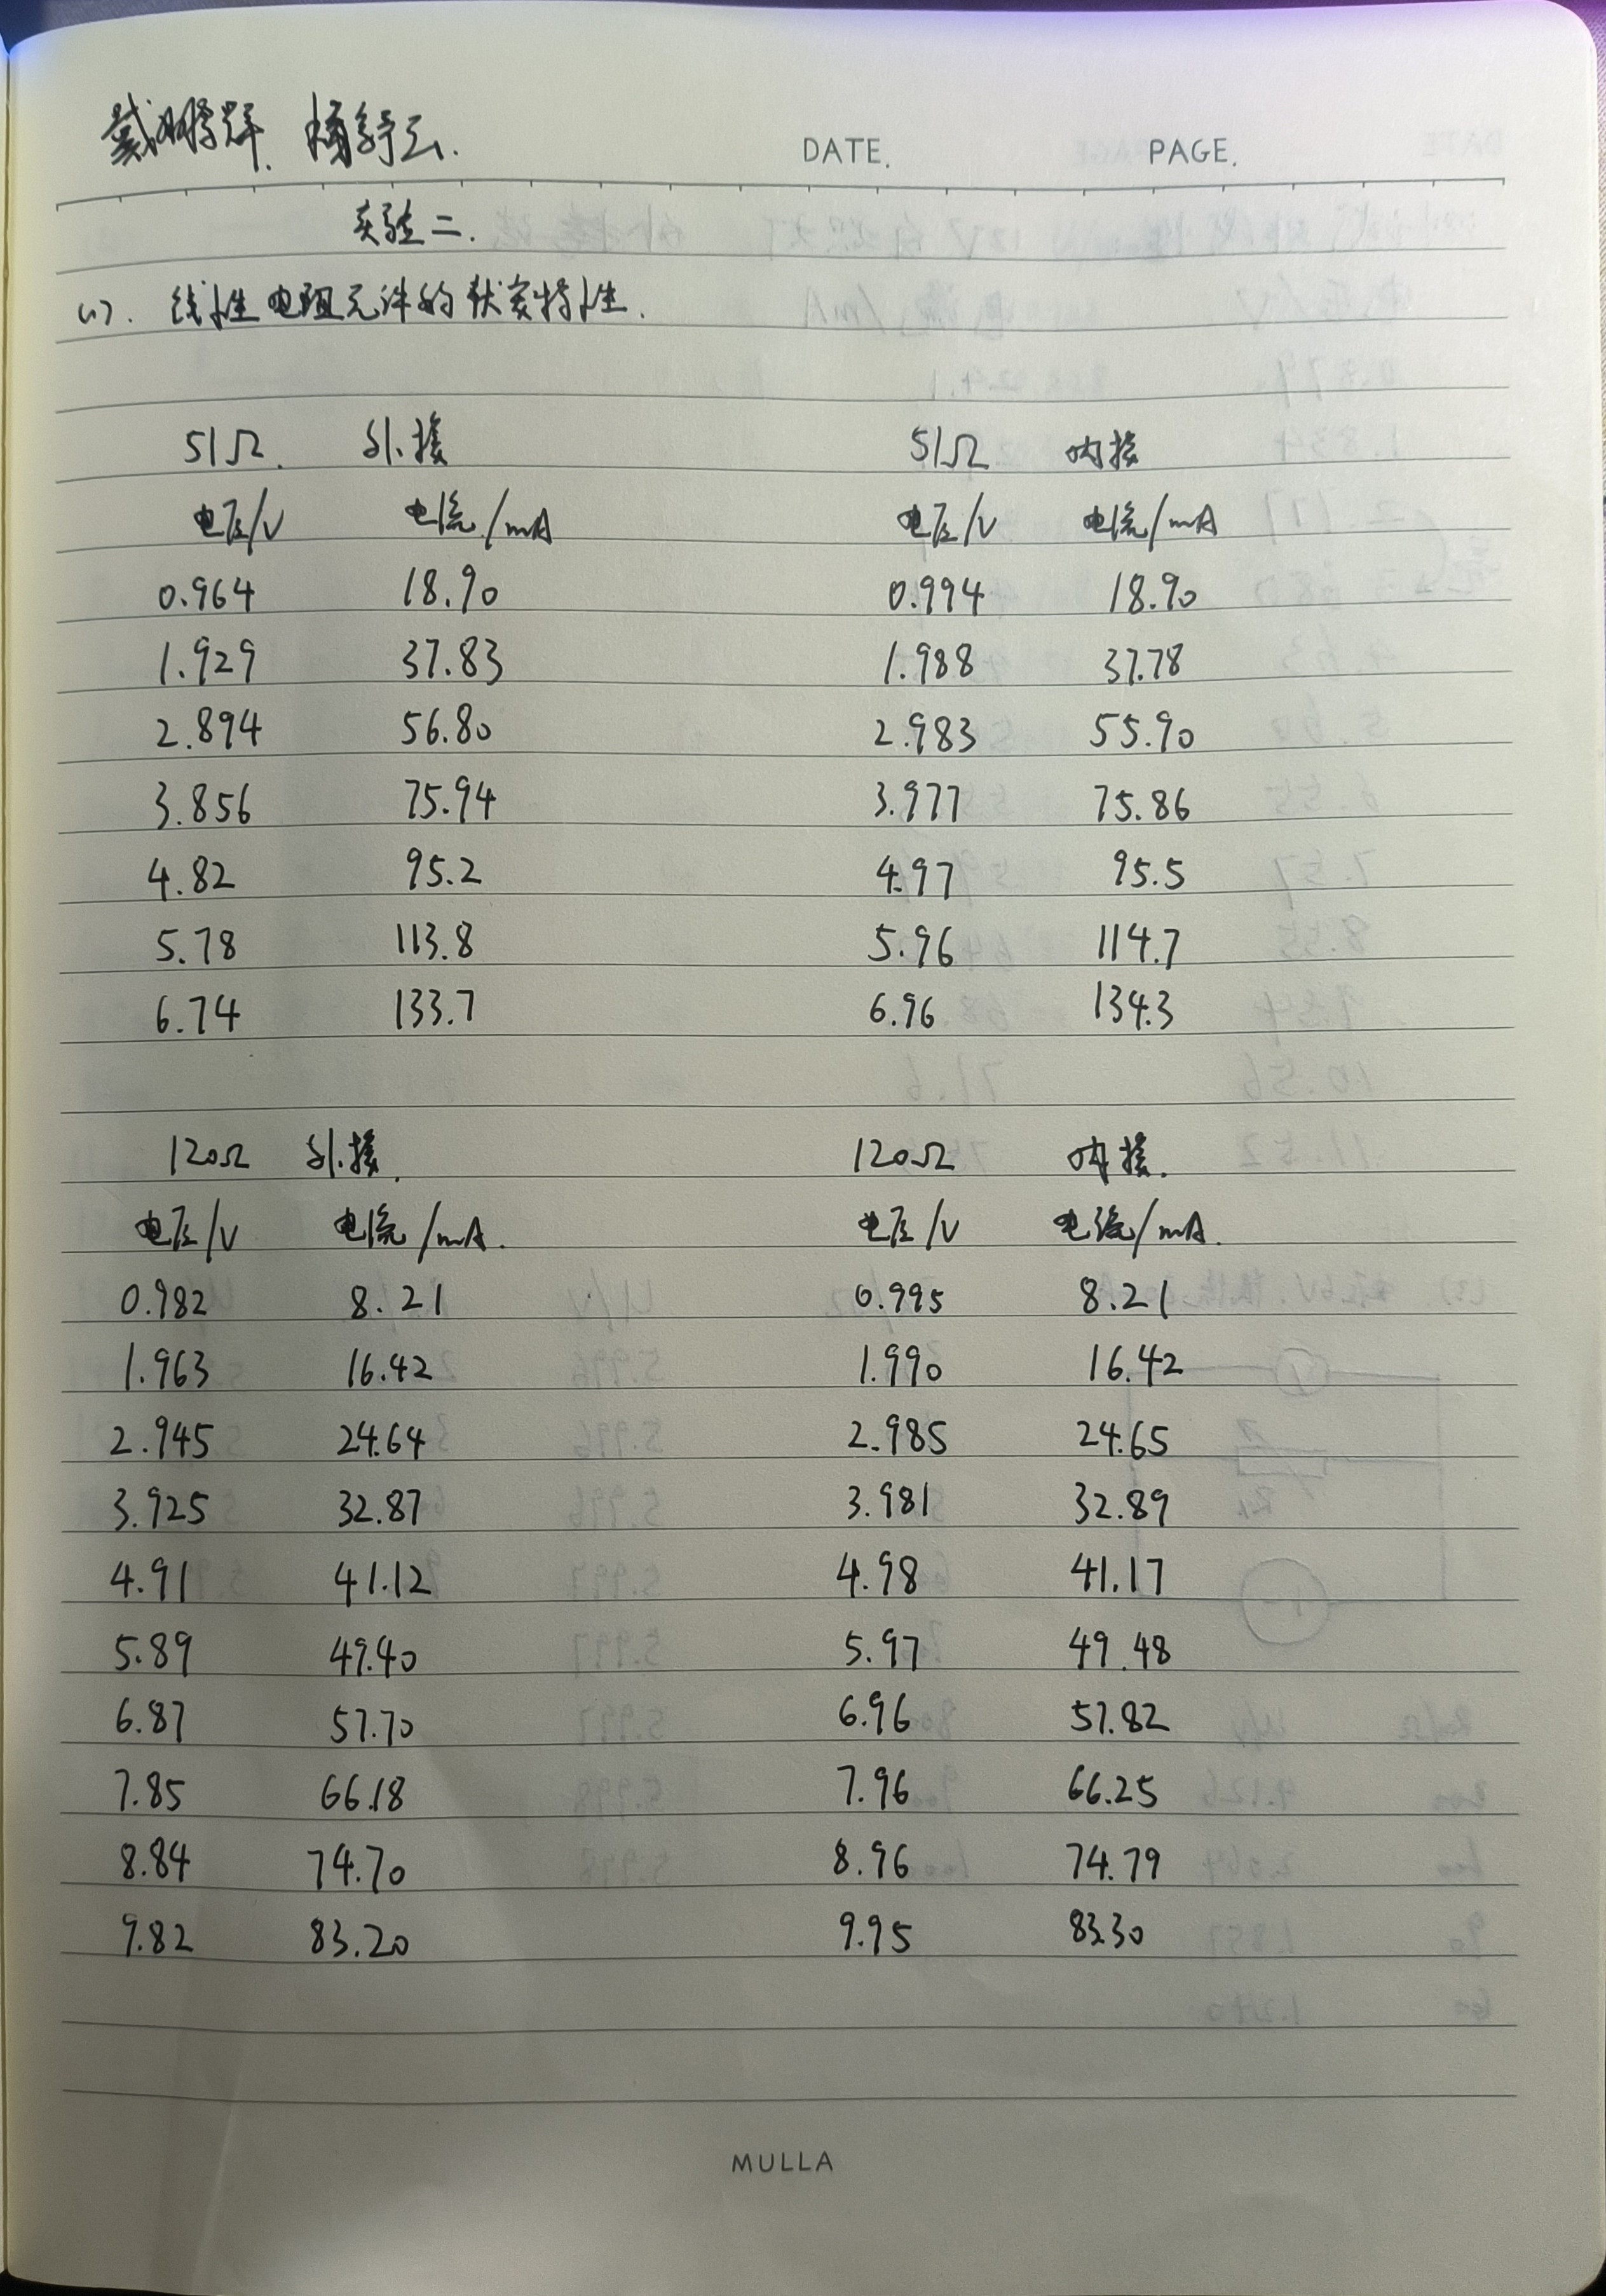
\includegraphics[width=0.32\textwidth]{ET1_2Gradata-1_reduce.jpg}\label{fig:figdata-1}}
		\quad
		\subfloat[原始数据2]
		{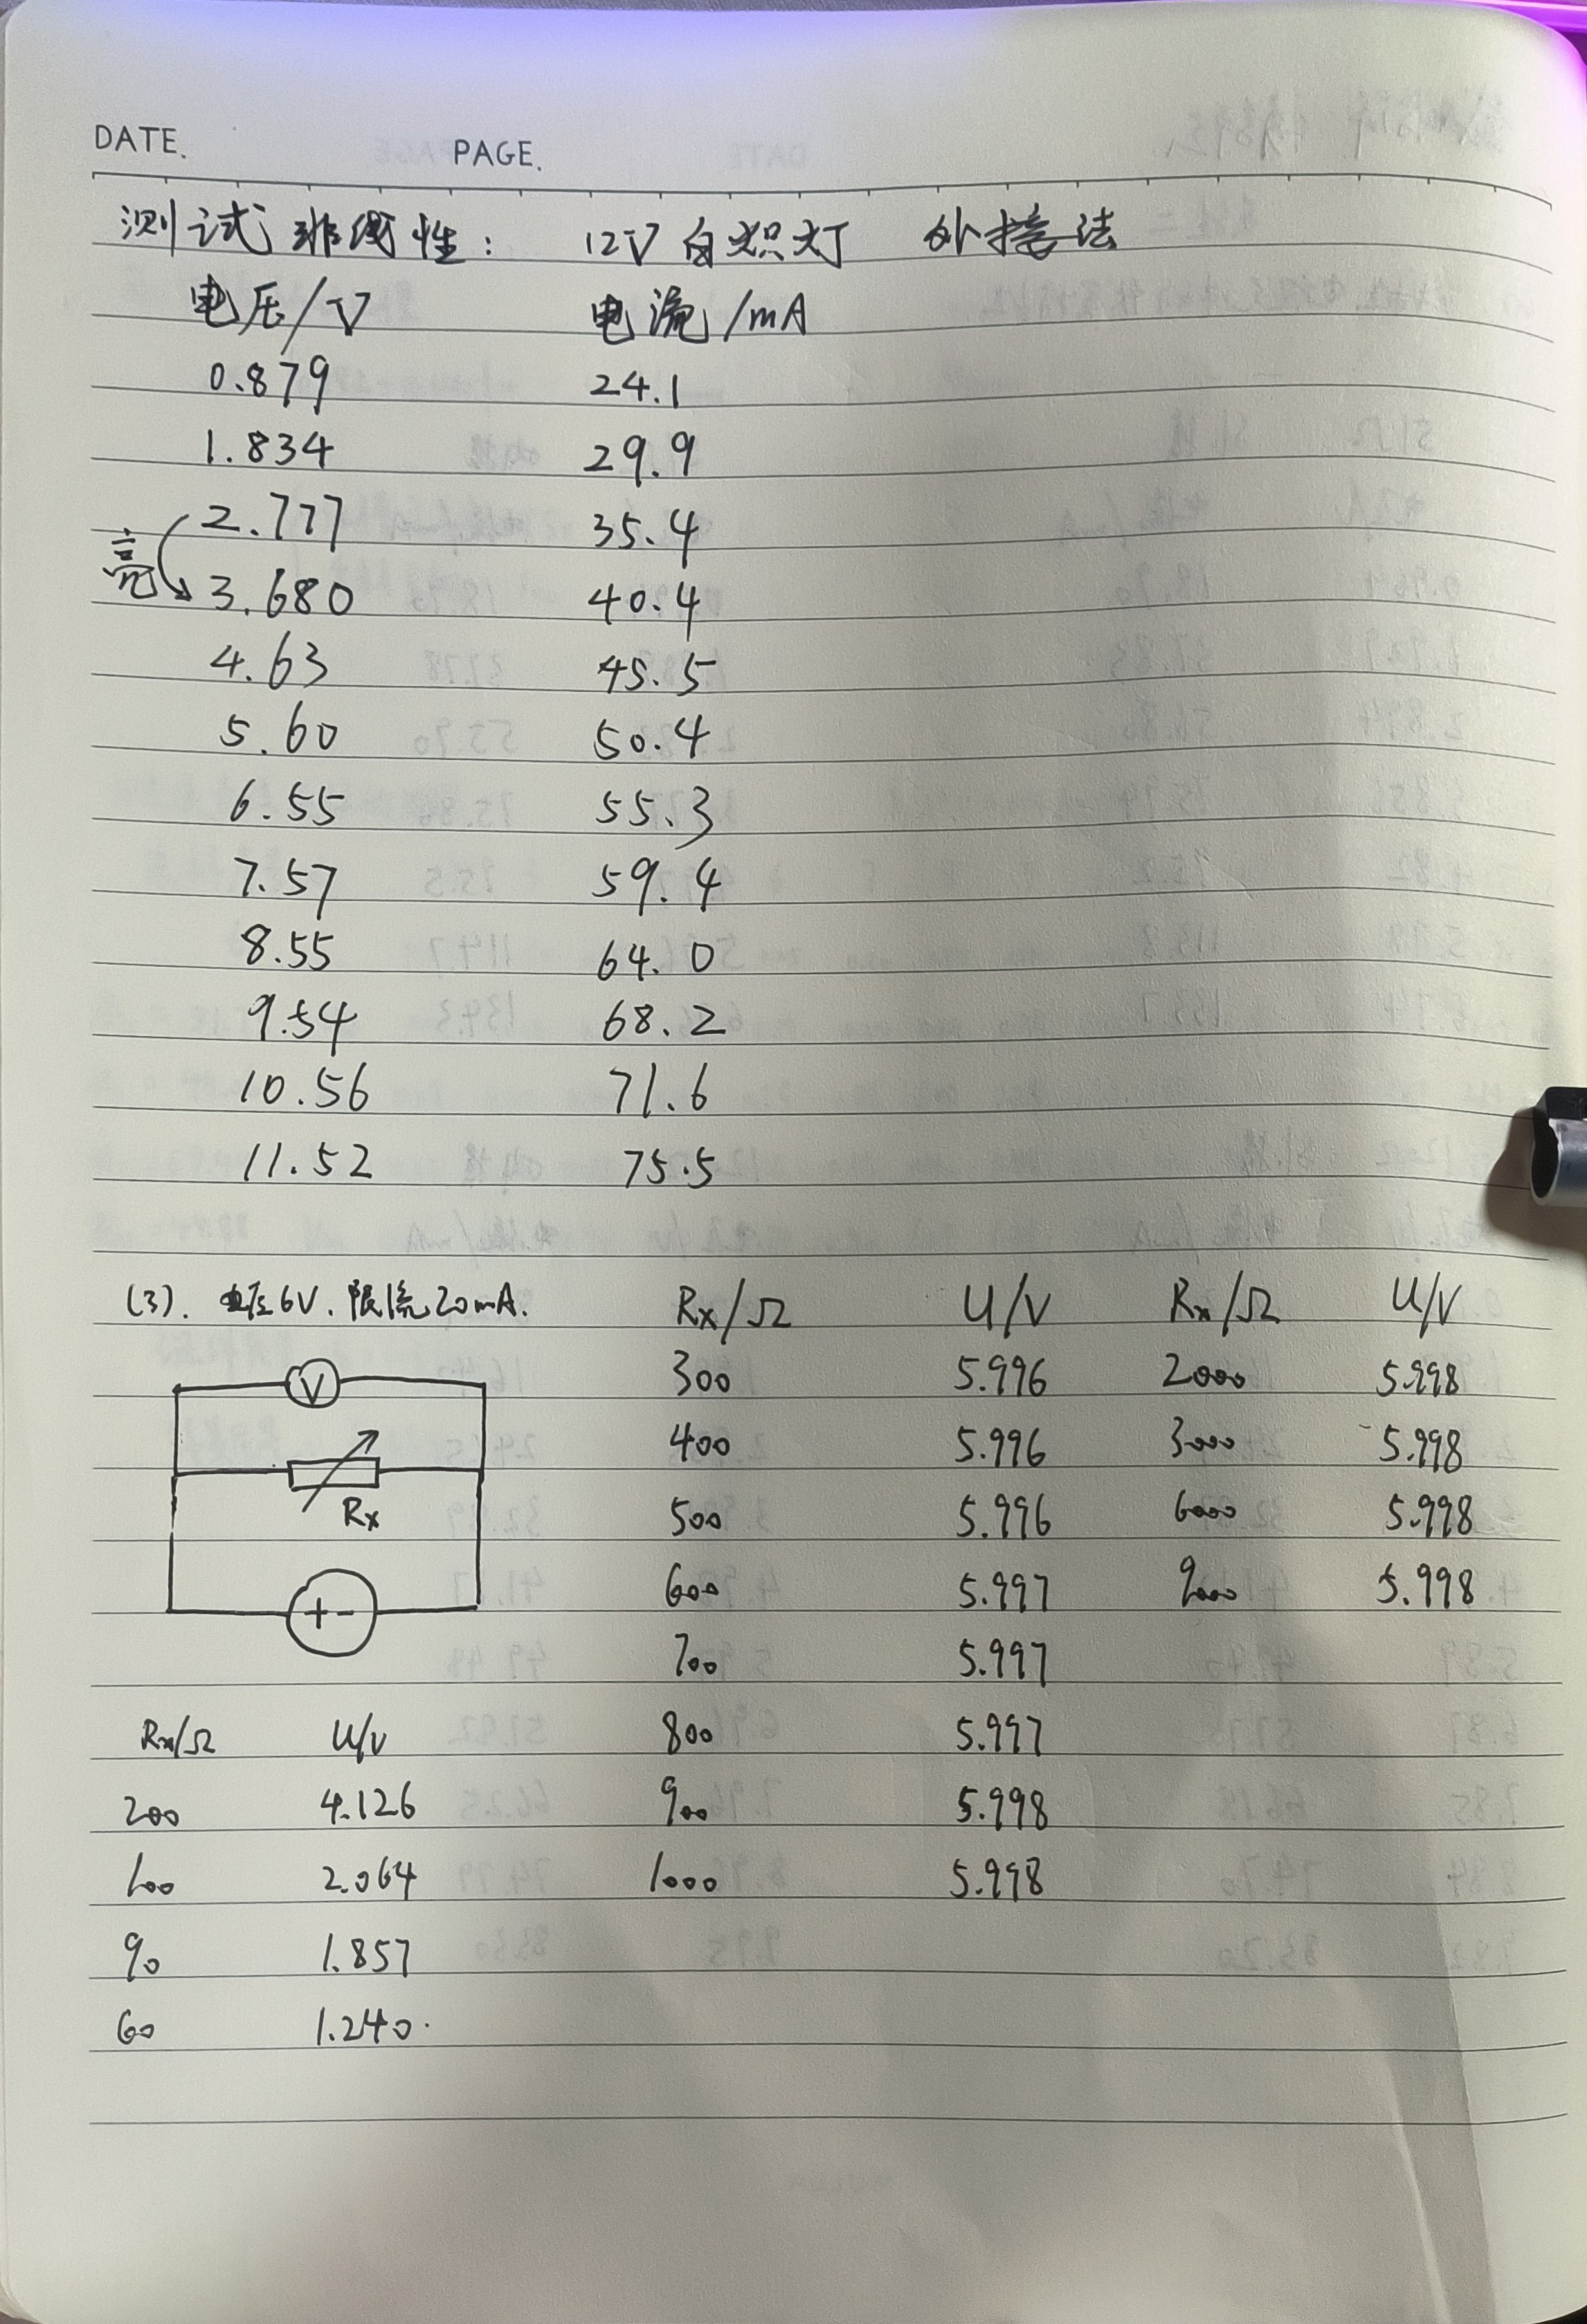
\includegraphics[width=0.32\textwidth]{ET1_2Gradata-2_reduce.jpg}\label{fig:figdata-2}}
		\quad
		\subfloat[原始数据3]
		{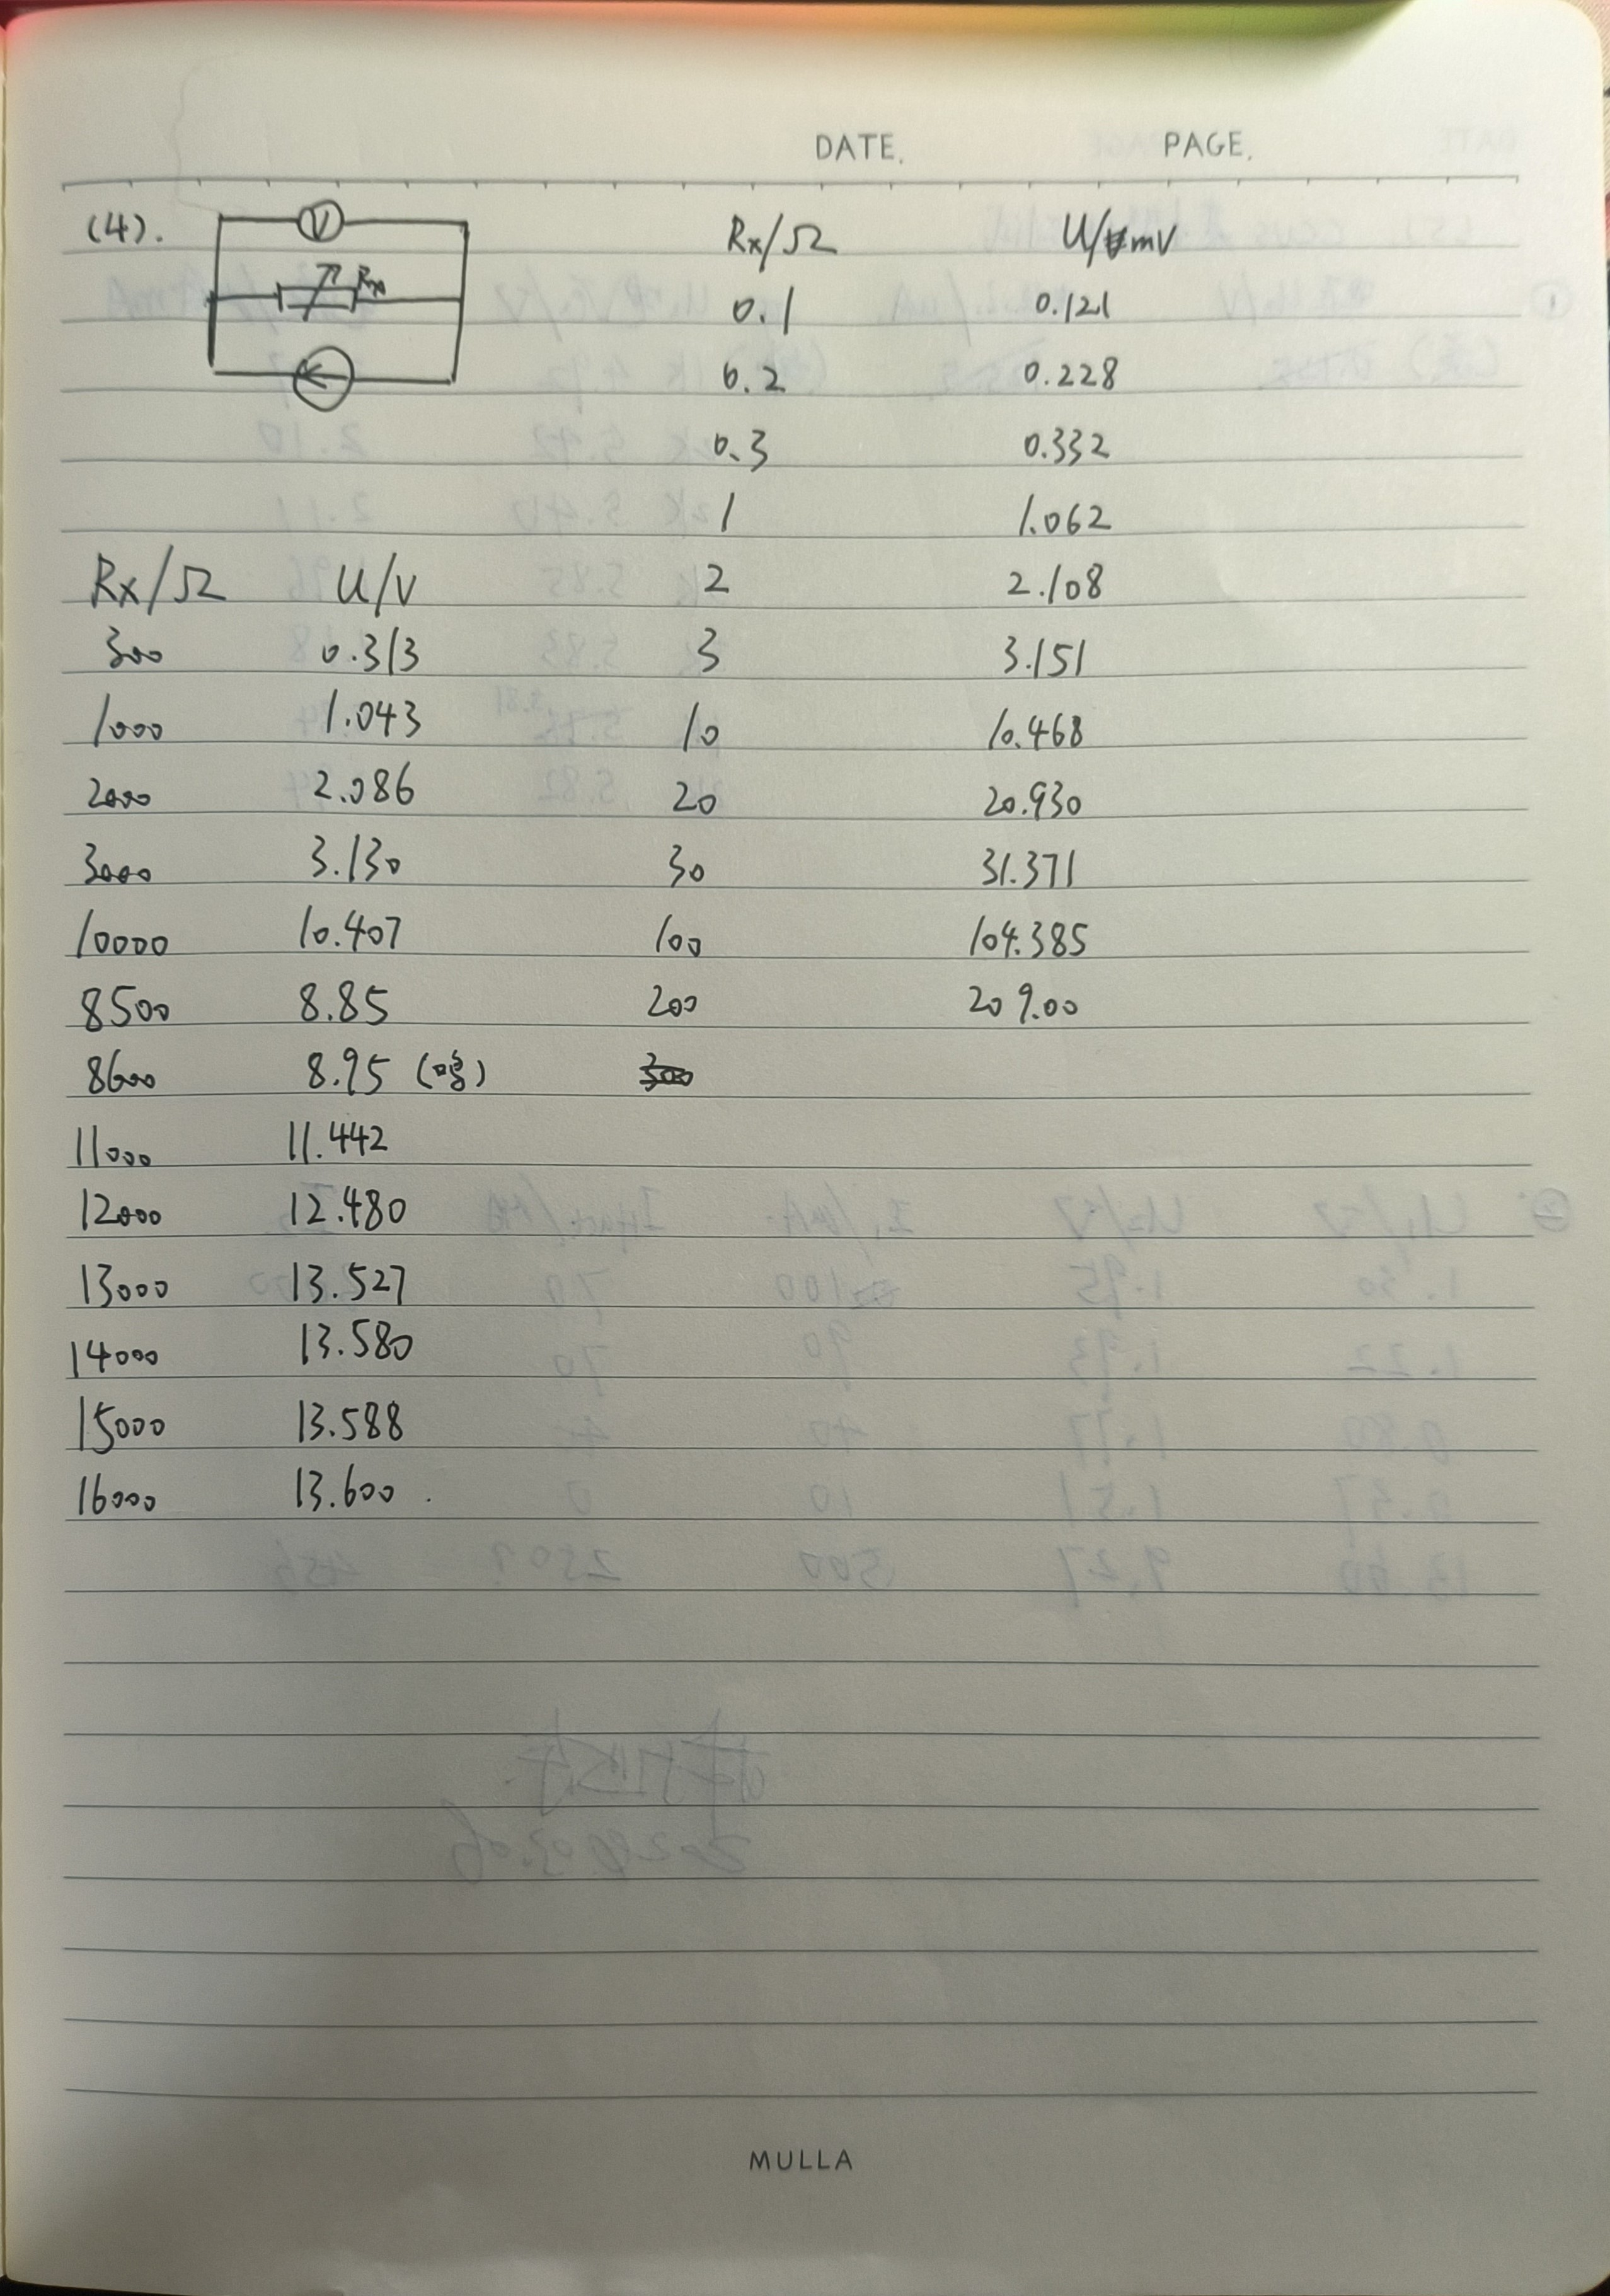
\includegraphics[width=0.32\textwidth]{ET1_2Gradata-3_reduce.jpg}\label{fig:figdata-3}}
		\quad
		\subfloat[原始数据4]
		{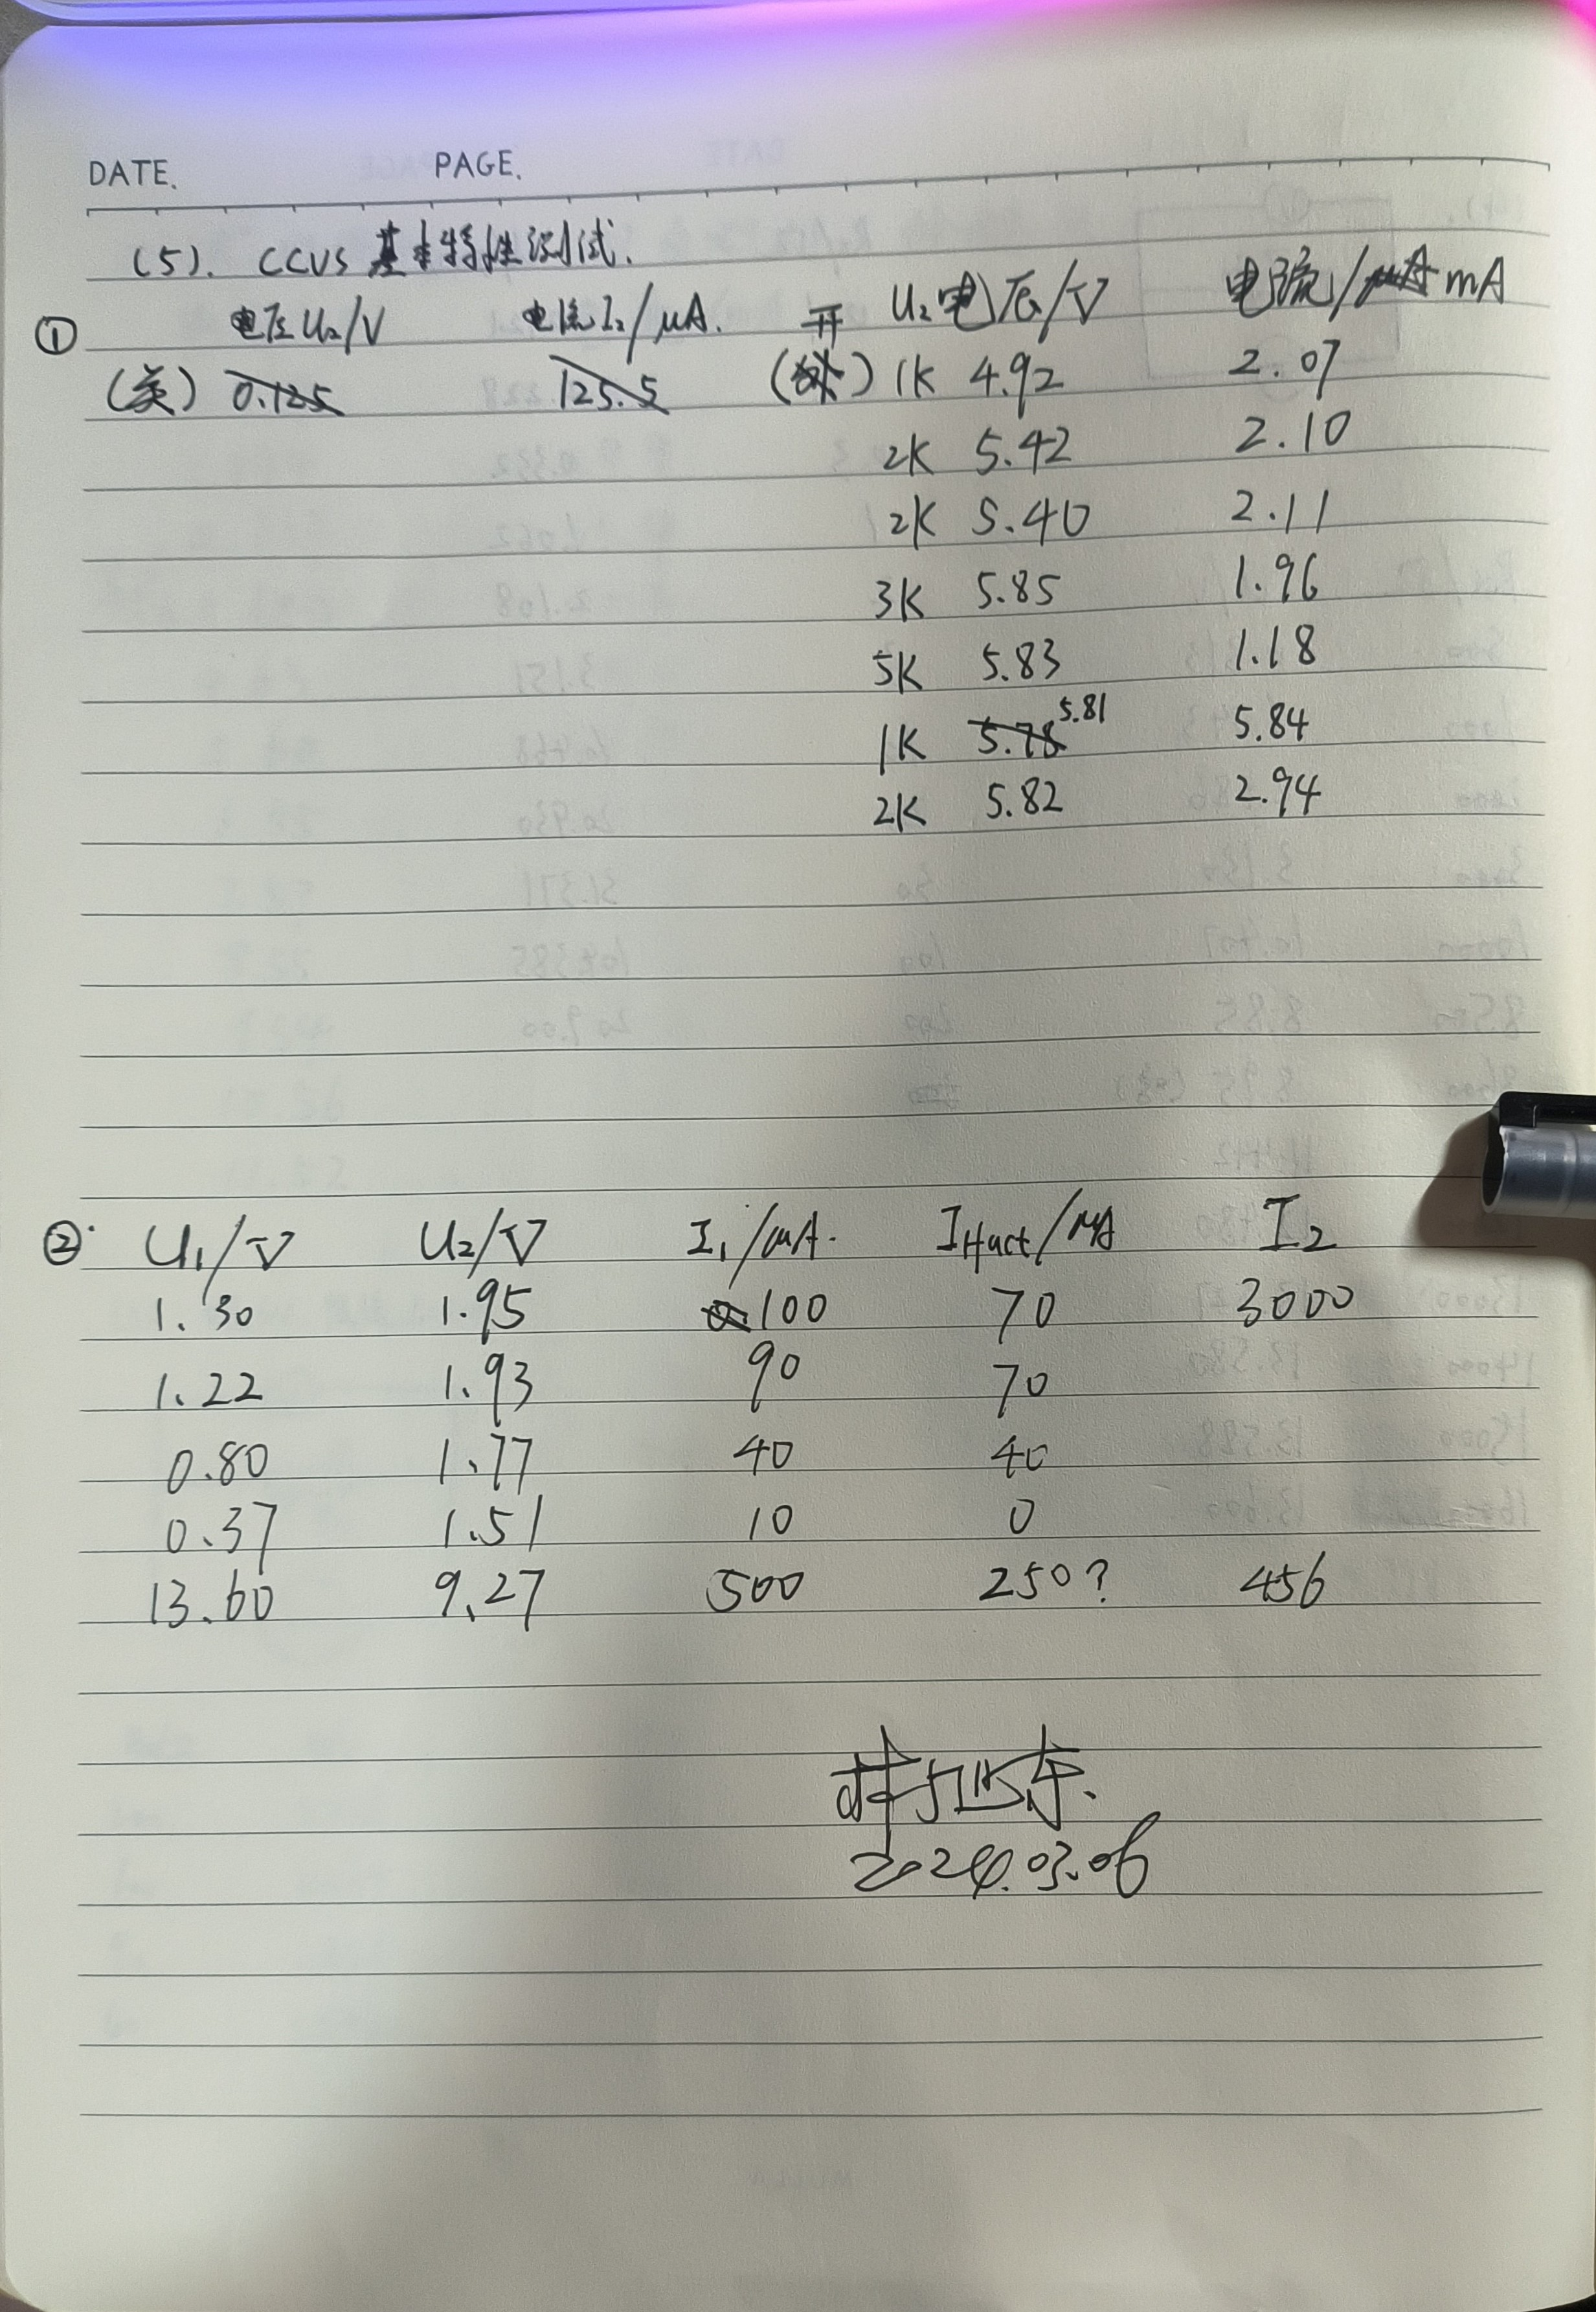
\includegraphics[width=0.32\textwidth]{ET1_2Gradata-4_reduce.jpg}\label{fig:figdata-4}}
		\quad
		% \caption{慧差实验结果图}
		\label{fig:graph10}
	\end{figure}


	% \begin{figure}[htbp]
	% 	\centering
	% 	\includegraphics[width=0.5\textwidth]{ET1_2Gradata-1.jpg}
	% 	\caption{原始数据1}
	% 	\label{fig:figdata-1}
	% \end{figure}
	
	% \begin{figure}[htbp]
	% 	\centering
	% 	\includegraphics[width=0.5\textwidth]{ET1_2Gradata-2.jpg}
	% 	\caption{原始数据2}
	% 	\label{fig:figdata-2}
	% \end{figure}
	
	% \begin{figure}[htbp]
	% 	\centering
	% 	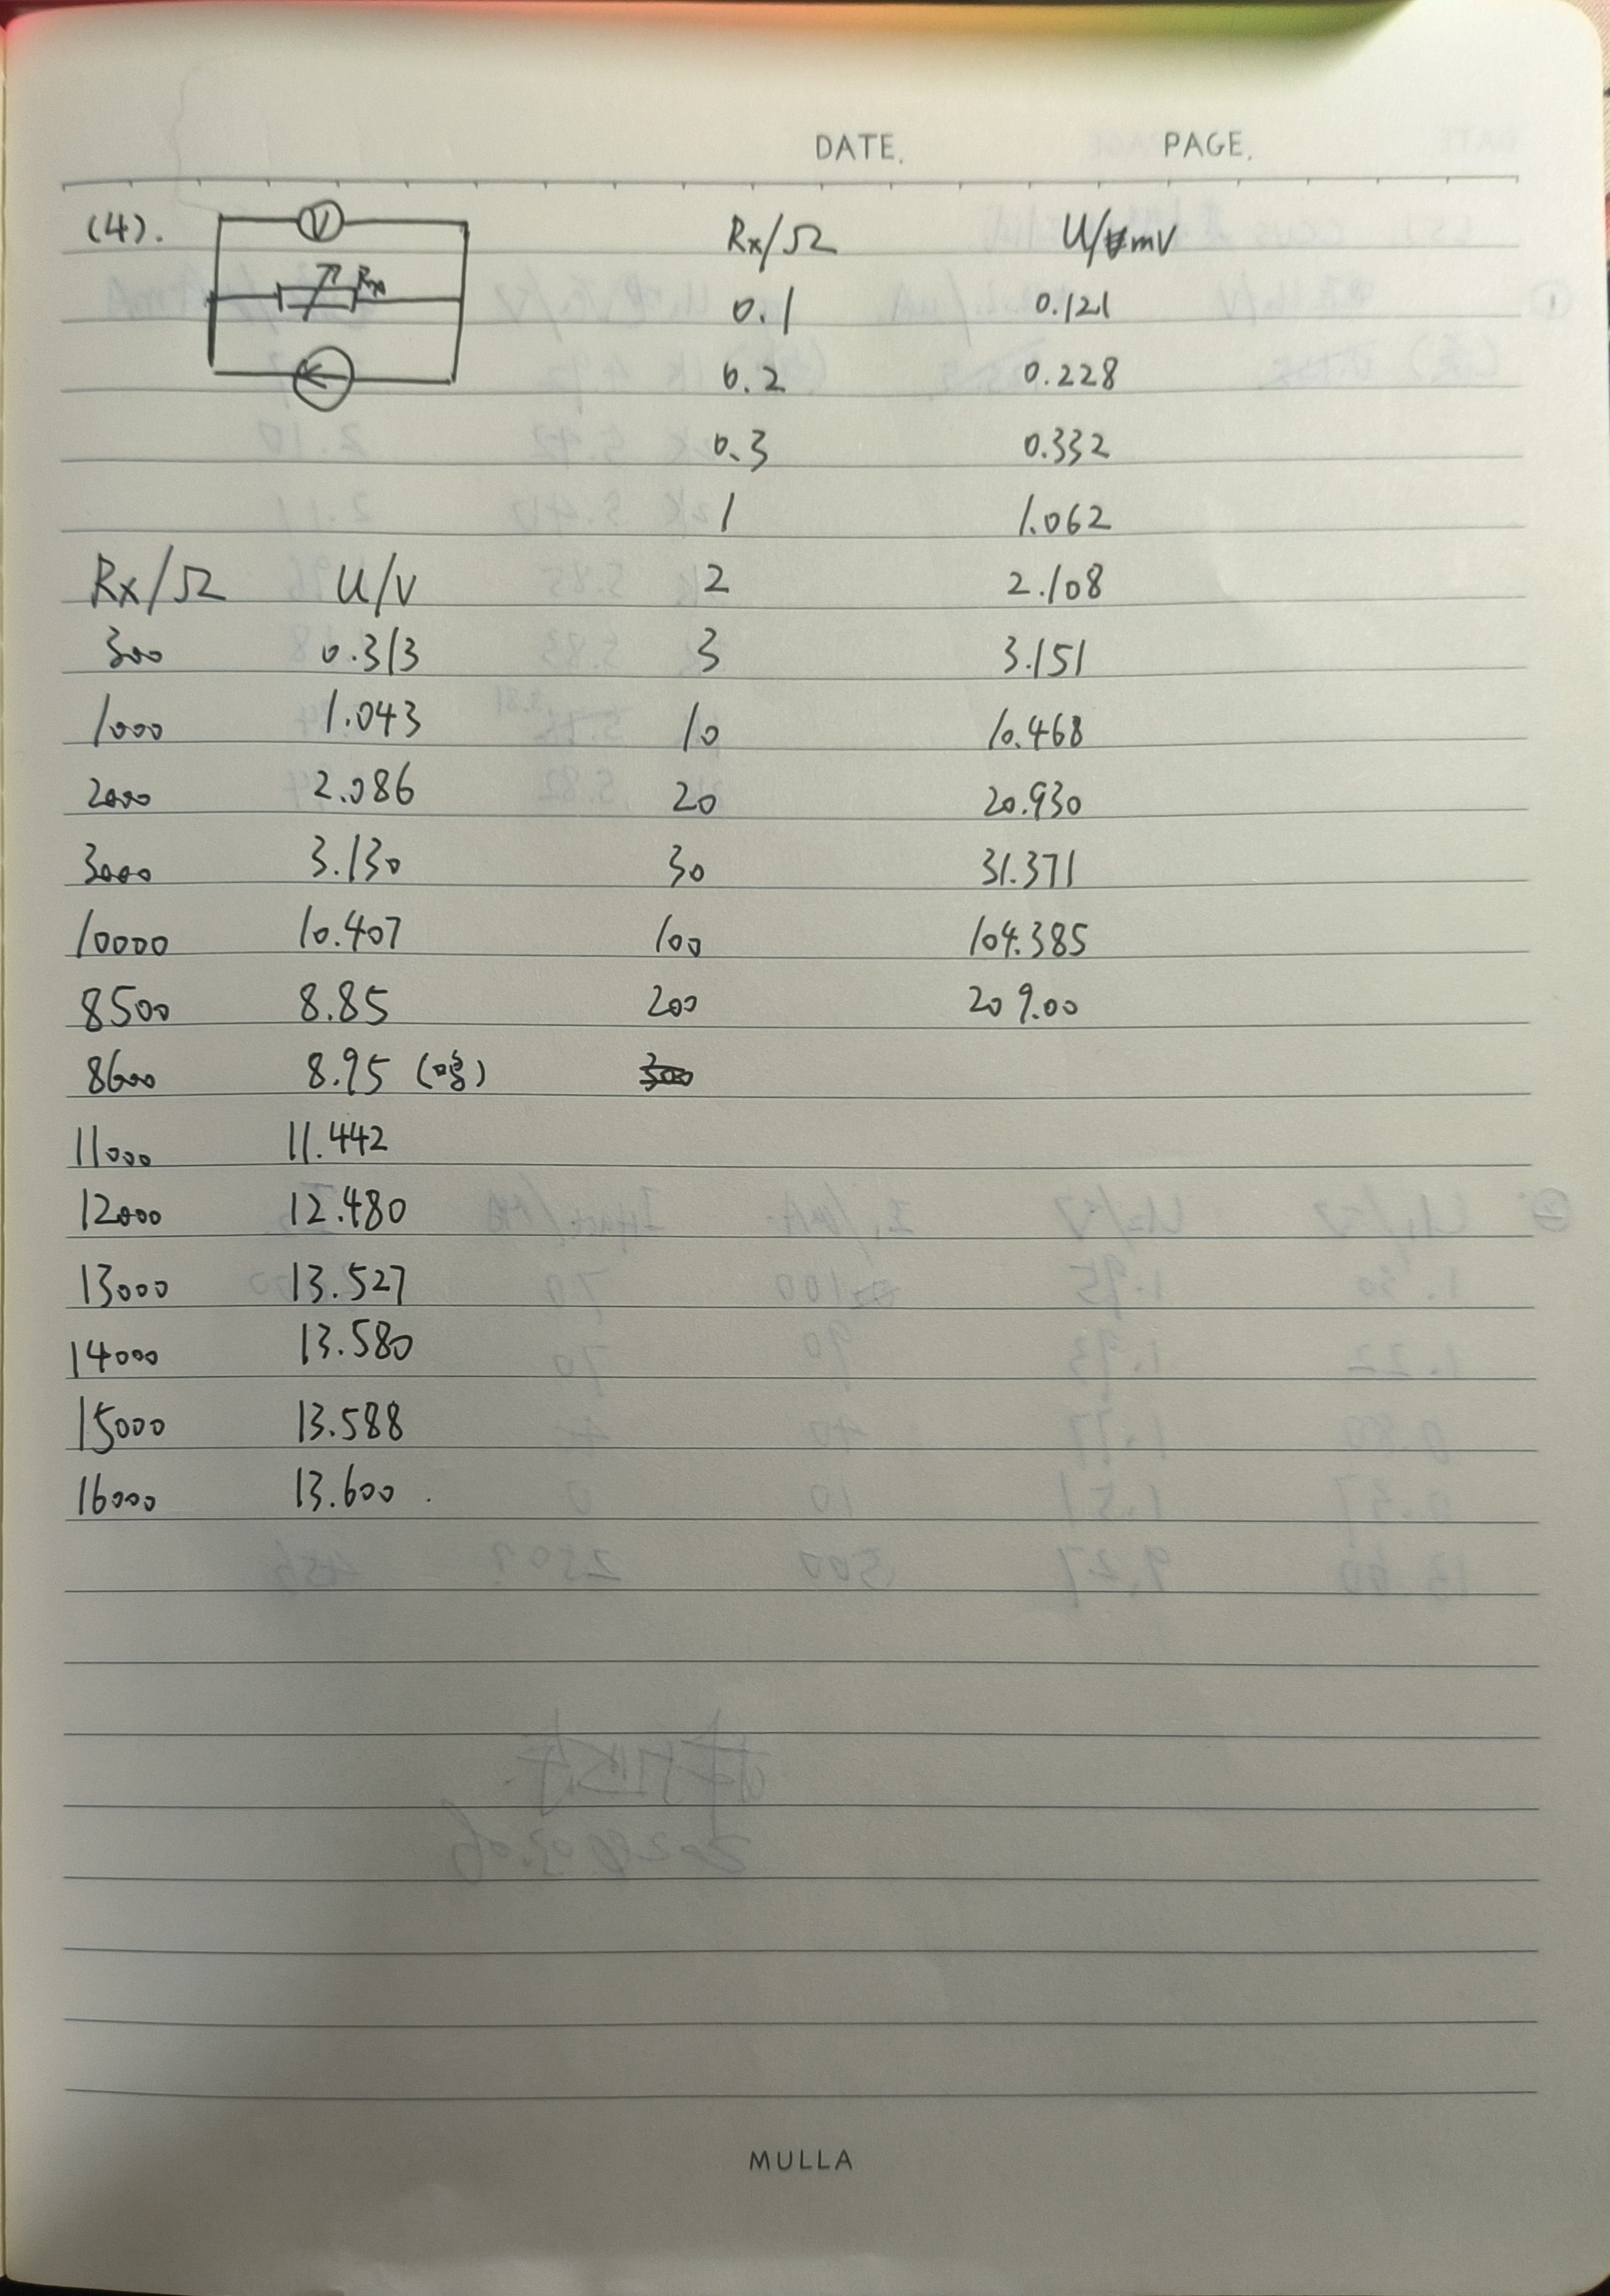
\includegraphics[width=0.5\textwidth]{ET1_2Gradata-3.jpg}
	% 	\caption{原始数据3}
	% 	\label{fig:figdata-3}
	% \end{figure}
	
	% \begin{figure}[htbp]
	% 	\centering
	% 	\includegraphics[width=0.5\textwidth]{ET1_2Gradata-4.jpg}
	% 	\caption{原始数据4}
	% 	\label{fig:figdata-4}
	% \end{figure}
	
	%实验台桌面整理见%\textbf{附件}部分(\cref{})。
	
	%其它原始数据见%\cref{}。
	% ---
	
	% 问题记录
	\subsection{实验过程遇到问题及解决办法}
	\begin{enumerate}
		\item 在测量受控源CCVS的实验时,因实验仪器的缘故,得到了偏离实验预期的结果。在后续与同学讨论后,确信这是CCCS,最后完成了实验。
	\end{enumerate}
	% ---
	
	
	
	% 分析与讨论	
	\clearpage
	
	% 顶栏
	\begin{table}
		\renewcommand\arraystretch{1.7}
		\begin{tabularx}{\textwidth}{|X|X|X|X|}
			\hline
			专业:& 物理学 &年级:& 2022级\\
			\hline
			姓名: & 戴鹏辉、杨舒云 & 学号:& 22344016、22344020\\
			\hline
			日期:& 2024/3/4 & 评分: &\\
			\hline
		\end{tabularx}
	\end{table}
	% ---
	
	% 小标题
	\section{实验二\quad 基本电路元件伏安特性的测量 \quad\heiti 分析与讨论}
	% ---
	
	% 数据处理
	\subsection{实验数据分析}
	
	%
	\subsubsection{各种元件的伏安特性曲线}
	\begin{enumerate}
		\item 测试线性电阻元件的伏安特性
		\begin{enumerate}
			\item 根据实验所测得到的数据,作出两个不同阻值电阻的伏案特性曲线,如\cref{fig:fig5}和\cref{fig:fig6}所示。
			
			\begin{figure}[htbp]
				\centering
				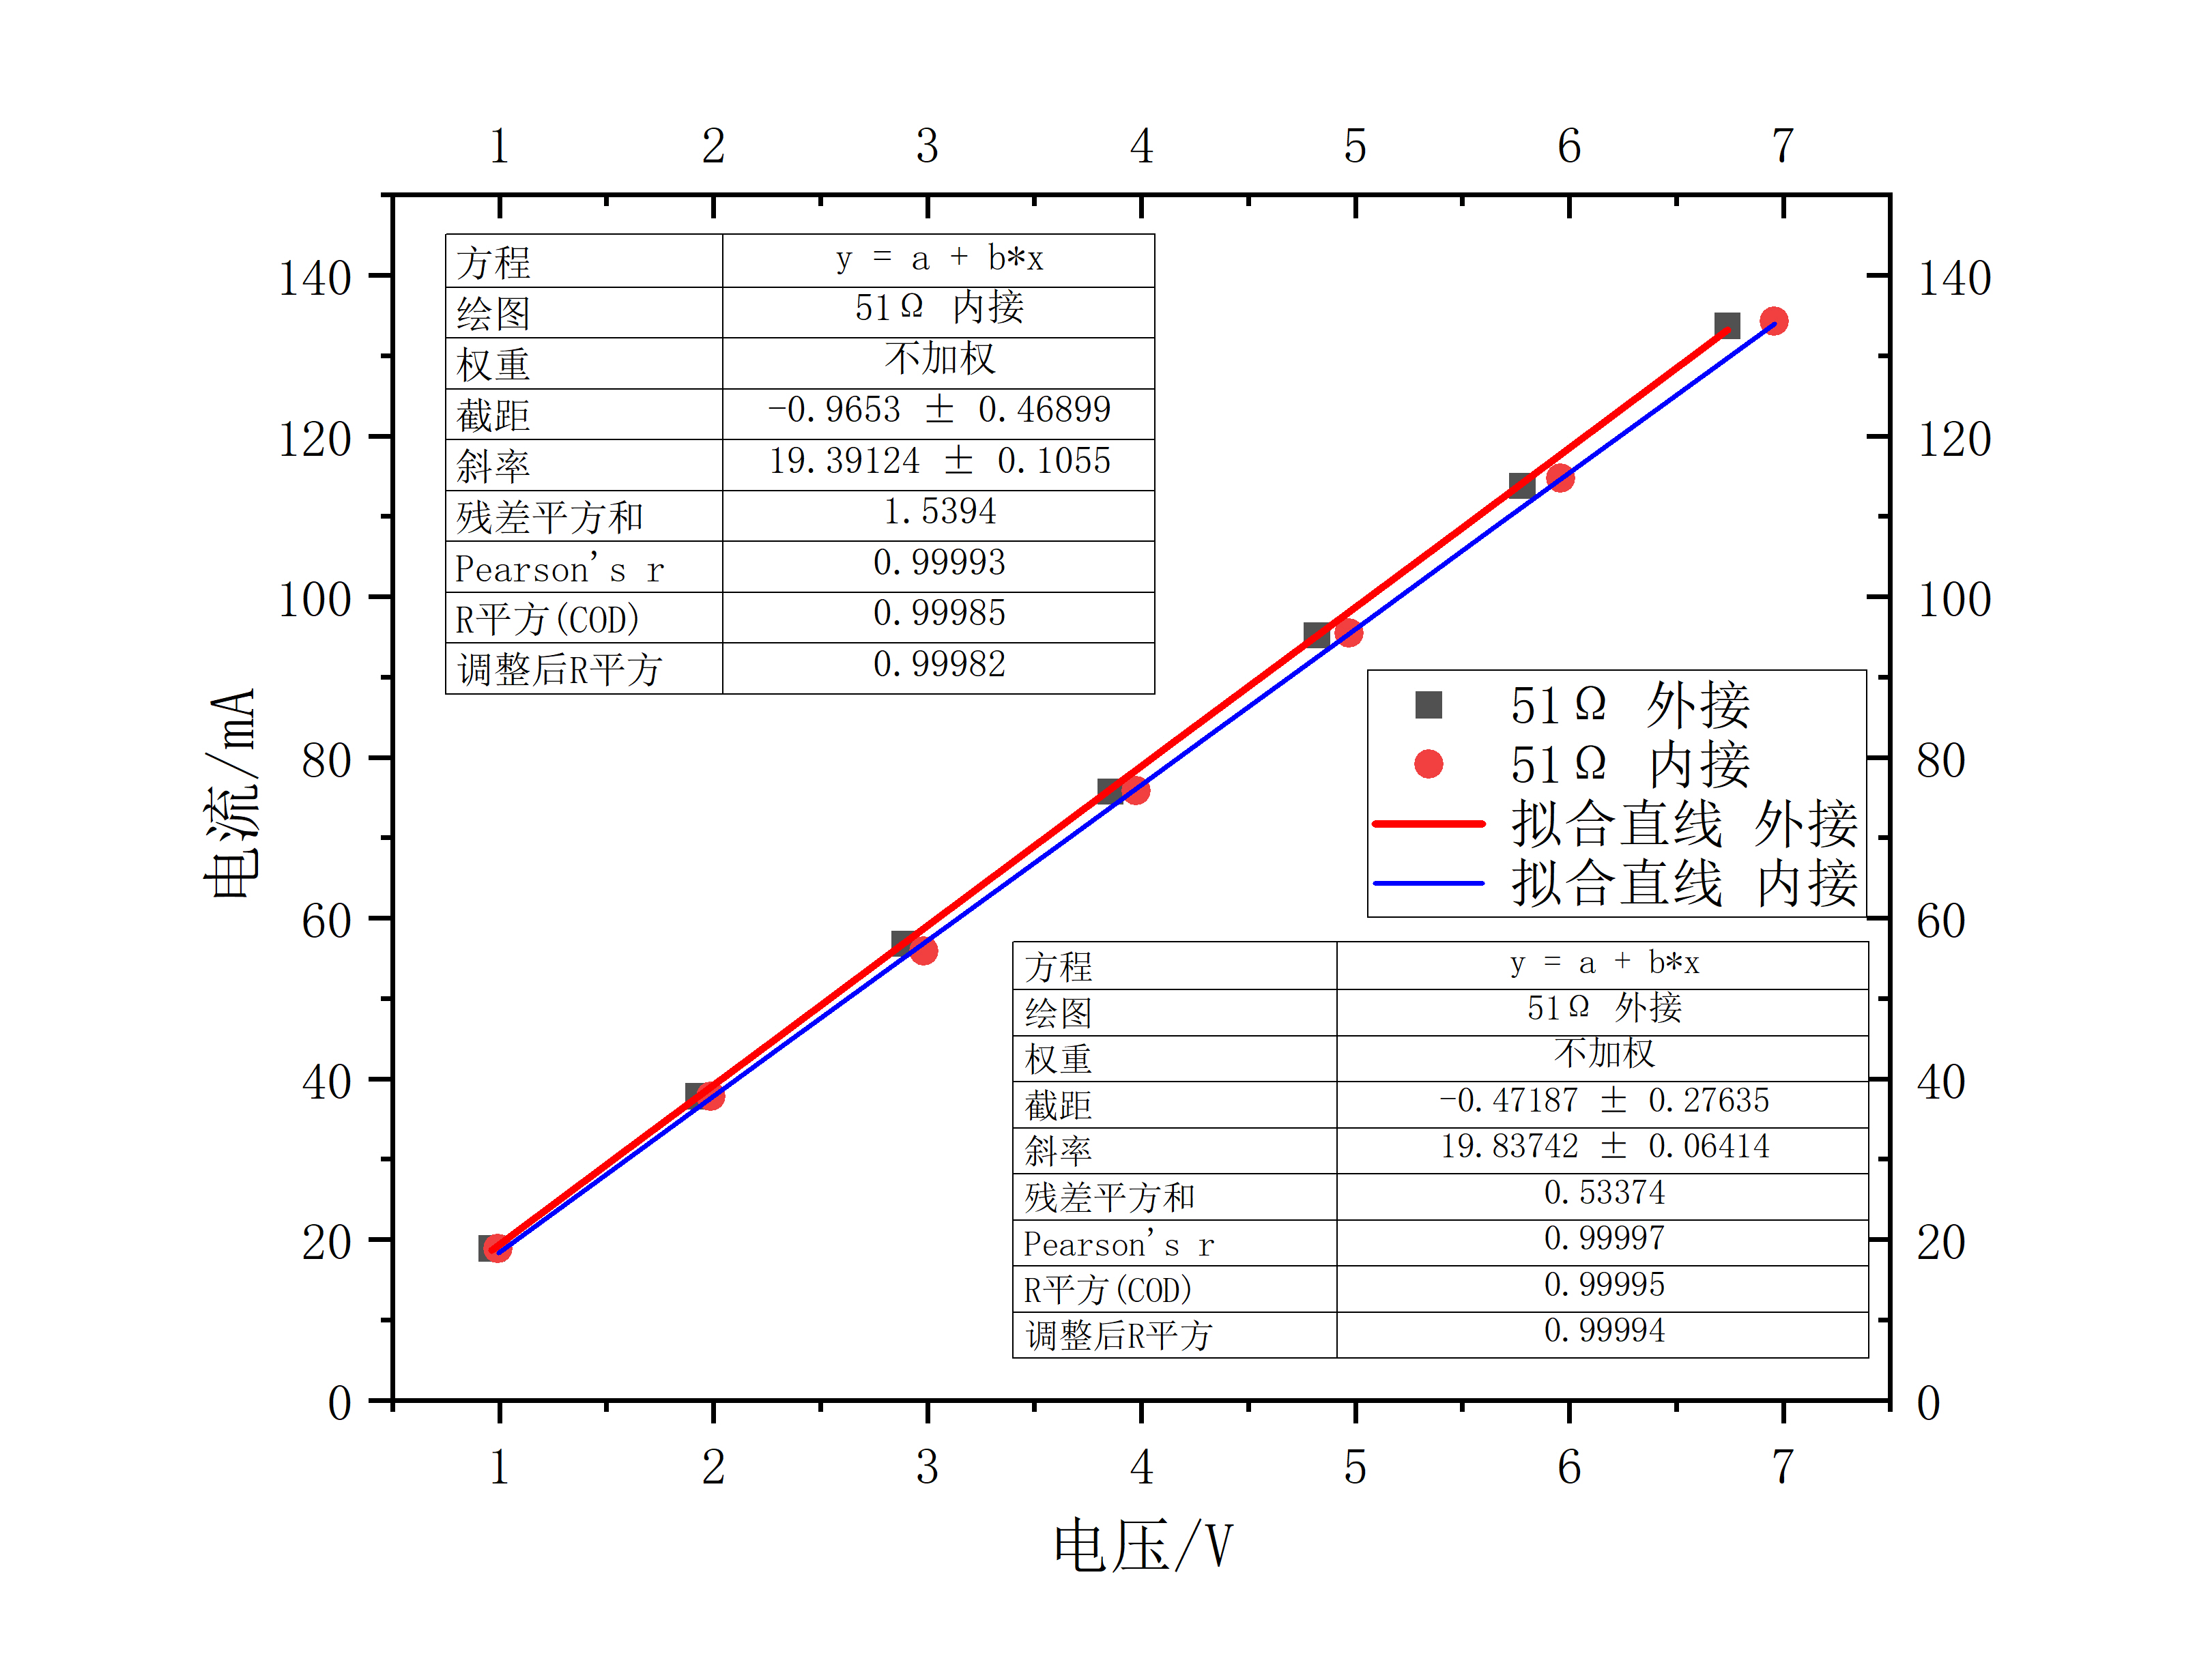
\includegraphics[width=0.7\textwidth]{ET1_2Gra5.jpg}
				\caption{51$\Omega$电阻伏安特性曲线}
				\label{fig:fig5}
			\end{figure}
			
			\begin{figure}[htbp]
				\centering
				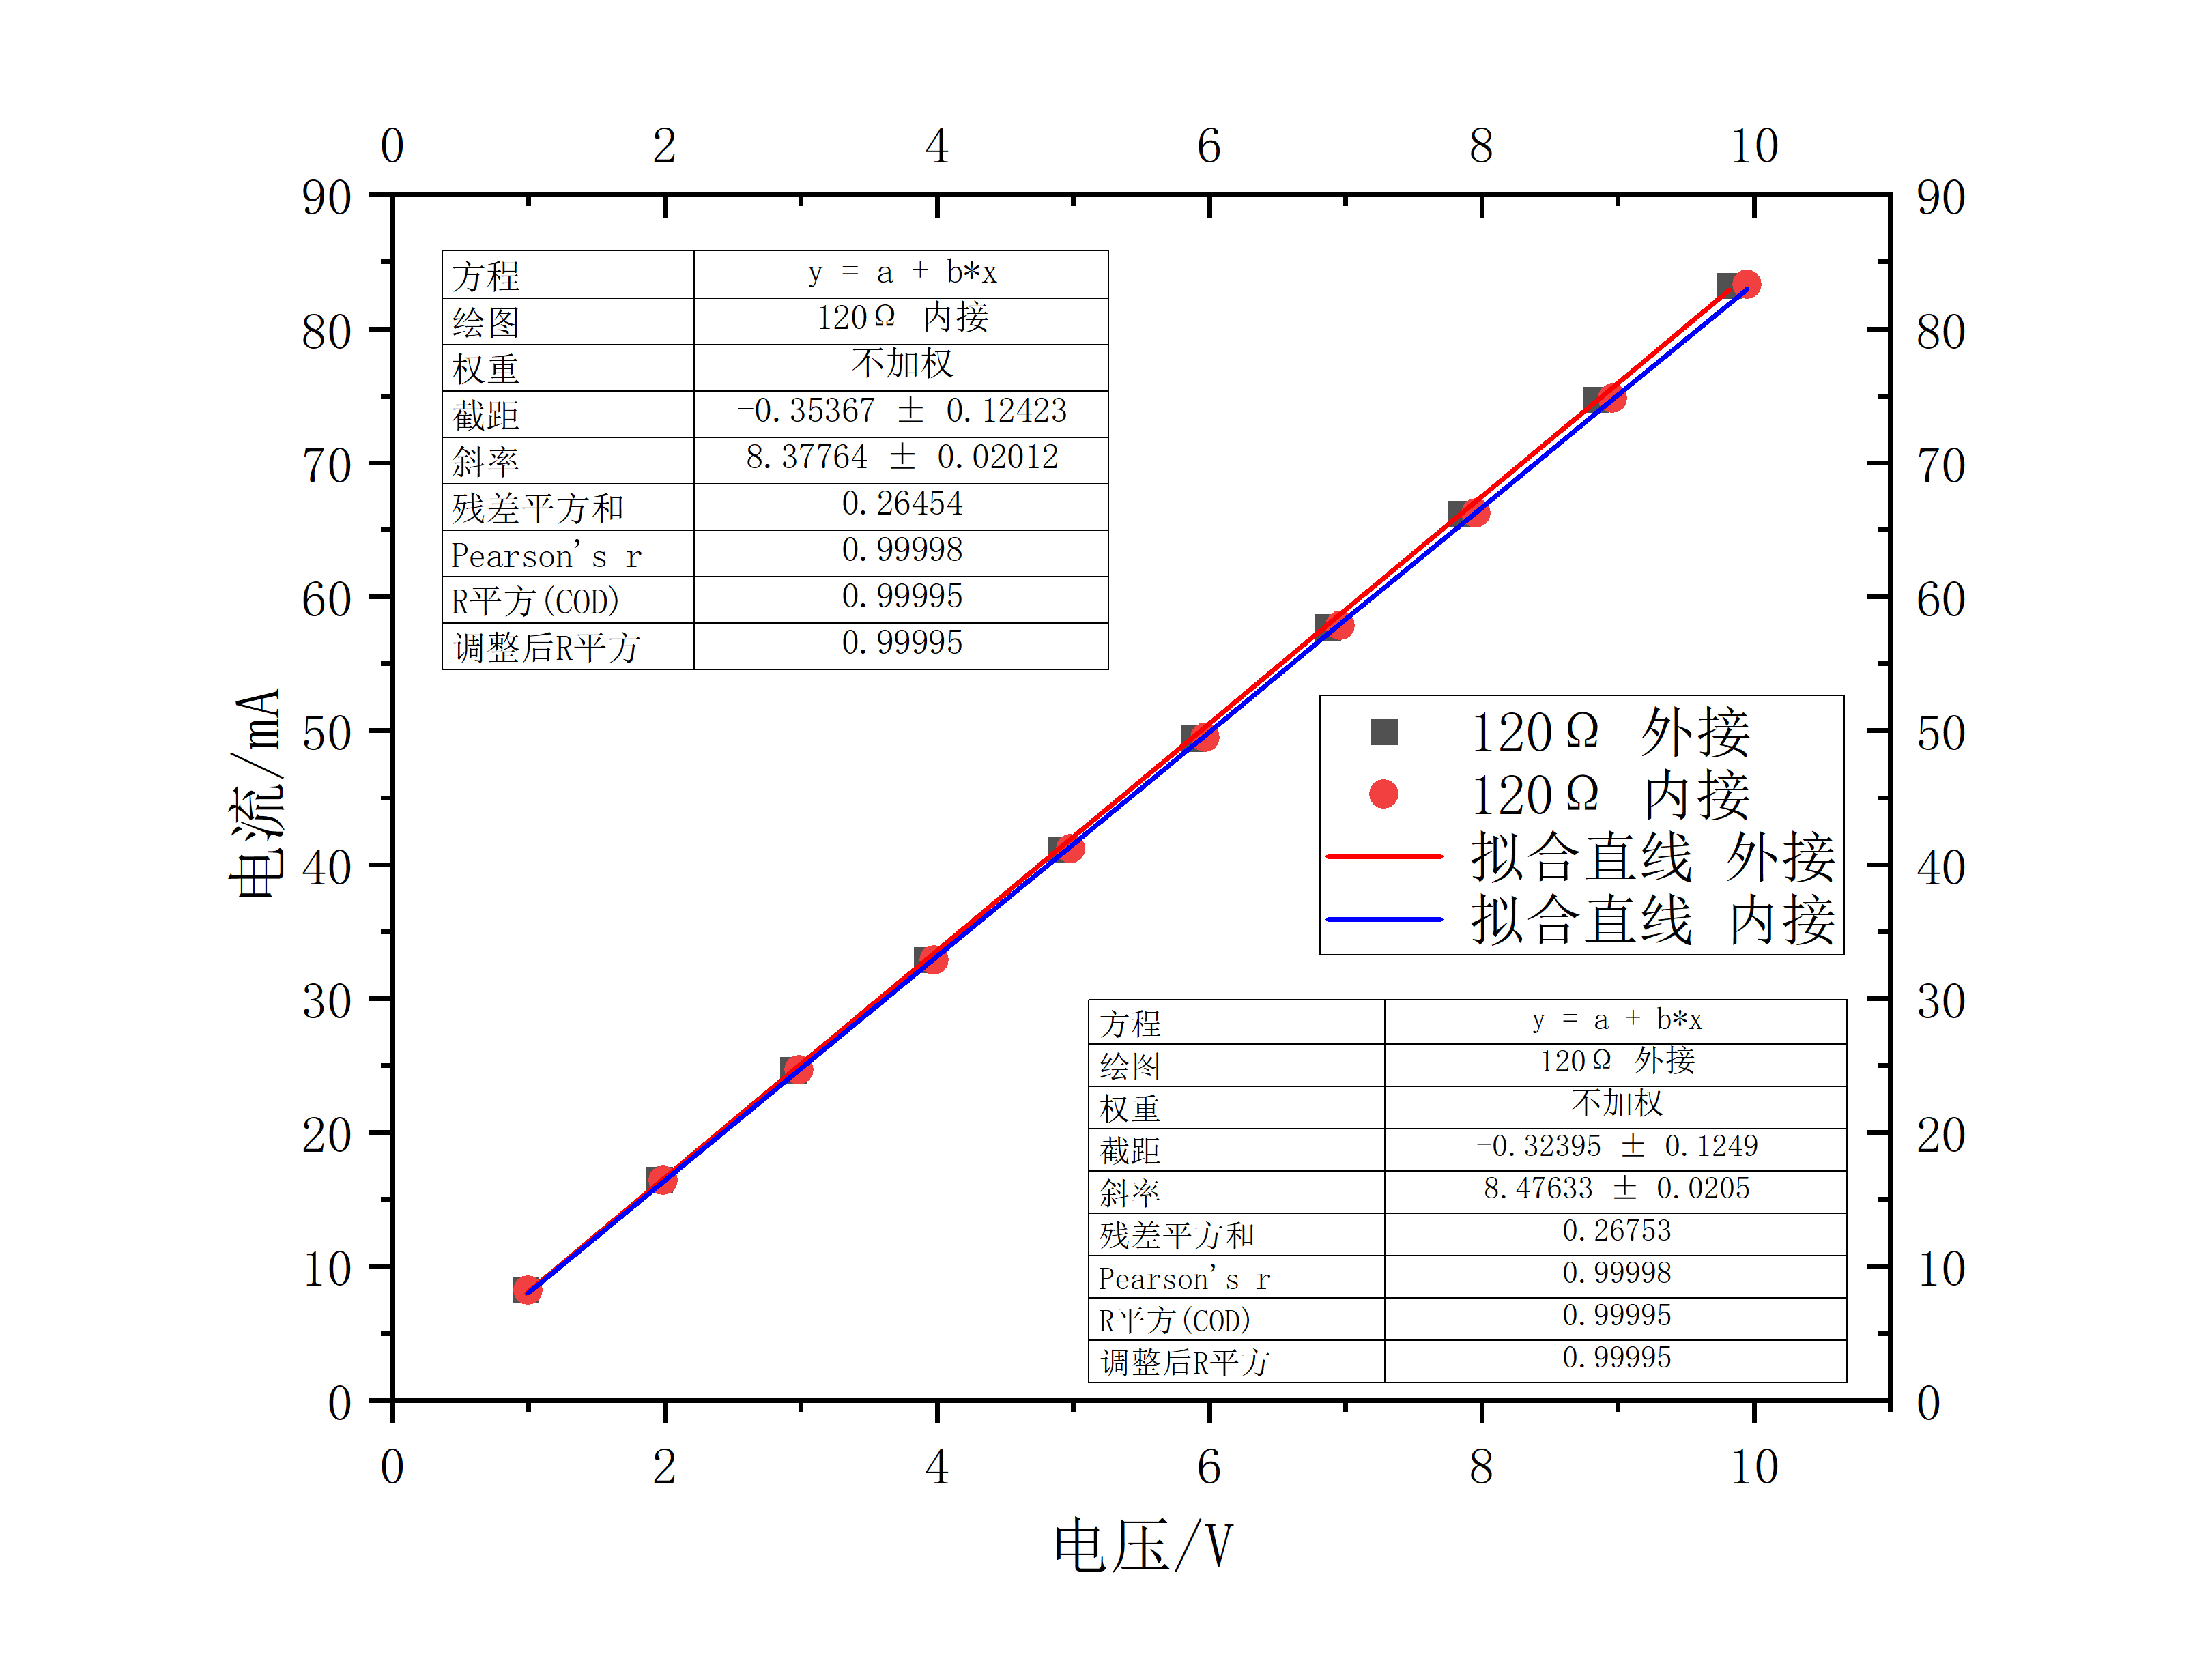
\includegraphics[width=0.7\textwidth]{ET1_2Gra6.jpg}
				\caption{120$\Omega$电阻伏安特性曲线}
				\label{fig:fig6}
			\end{figure}
			
			\item 根据各图的伏安特性曲线,可以通过斜率得到各电阻的实验测定值,详见下一个小节。
		\end{enumerate}
				
		\item 测试非线性电阻 12V 白炽灯的伏安特性
		\begin{enumerate}
			\item 根据实验所测得到的数据,白炽灯的伏安特性曲线作图如\cref{fig:fig7}所示。
			
			\begin{figure}[htbp]
				\centering
				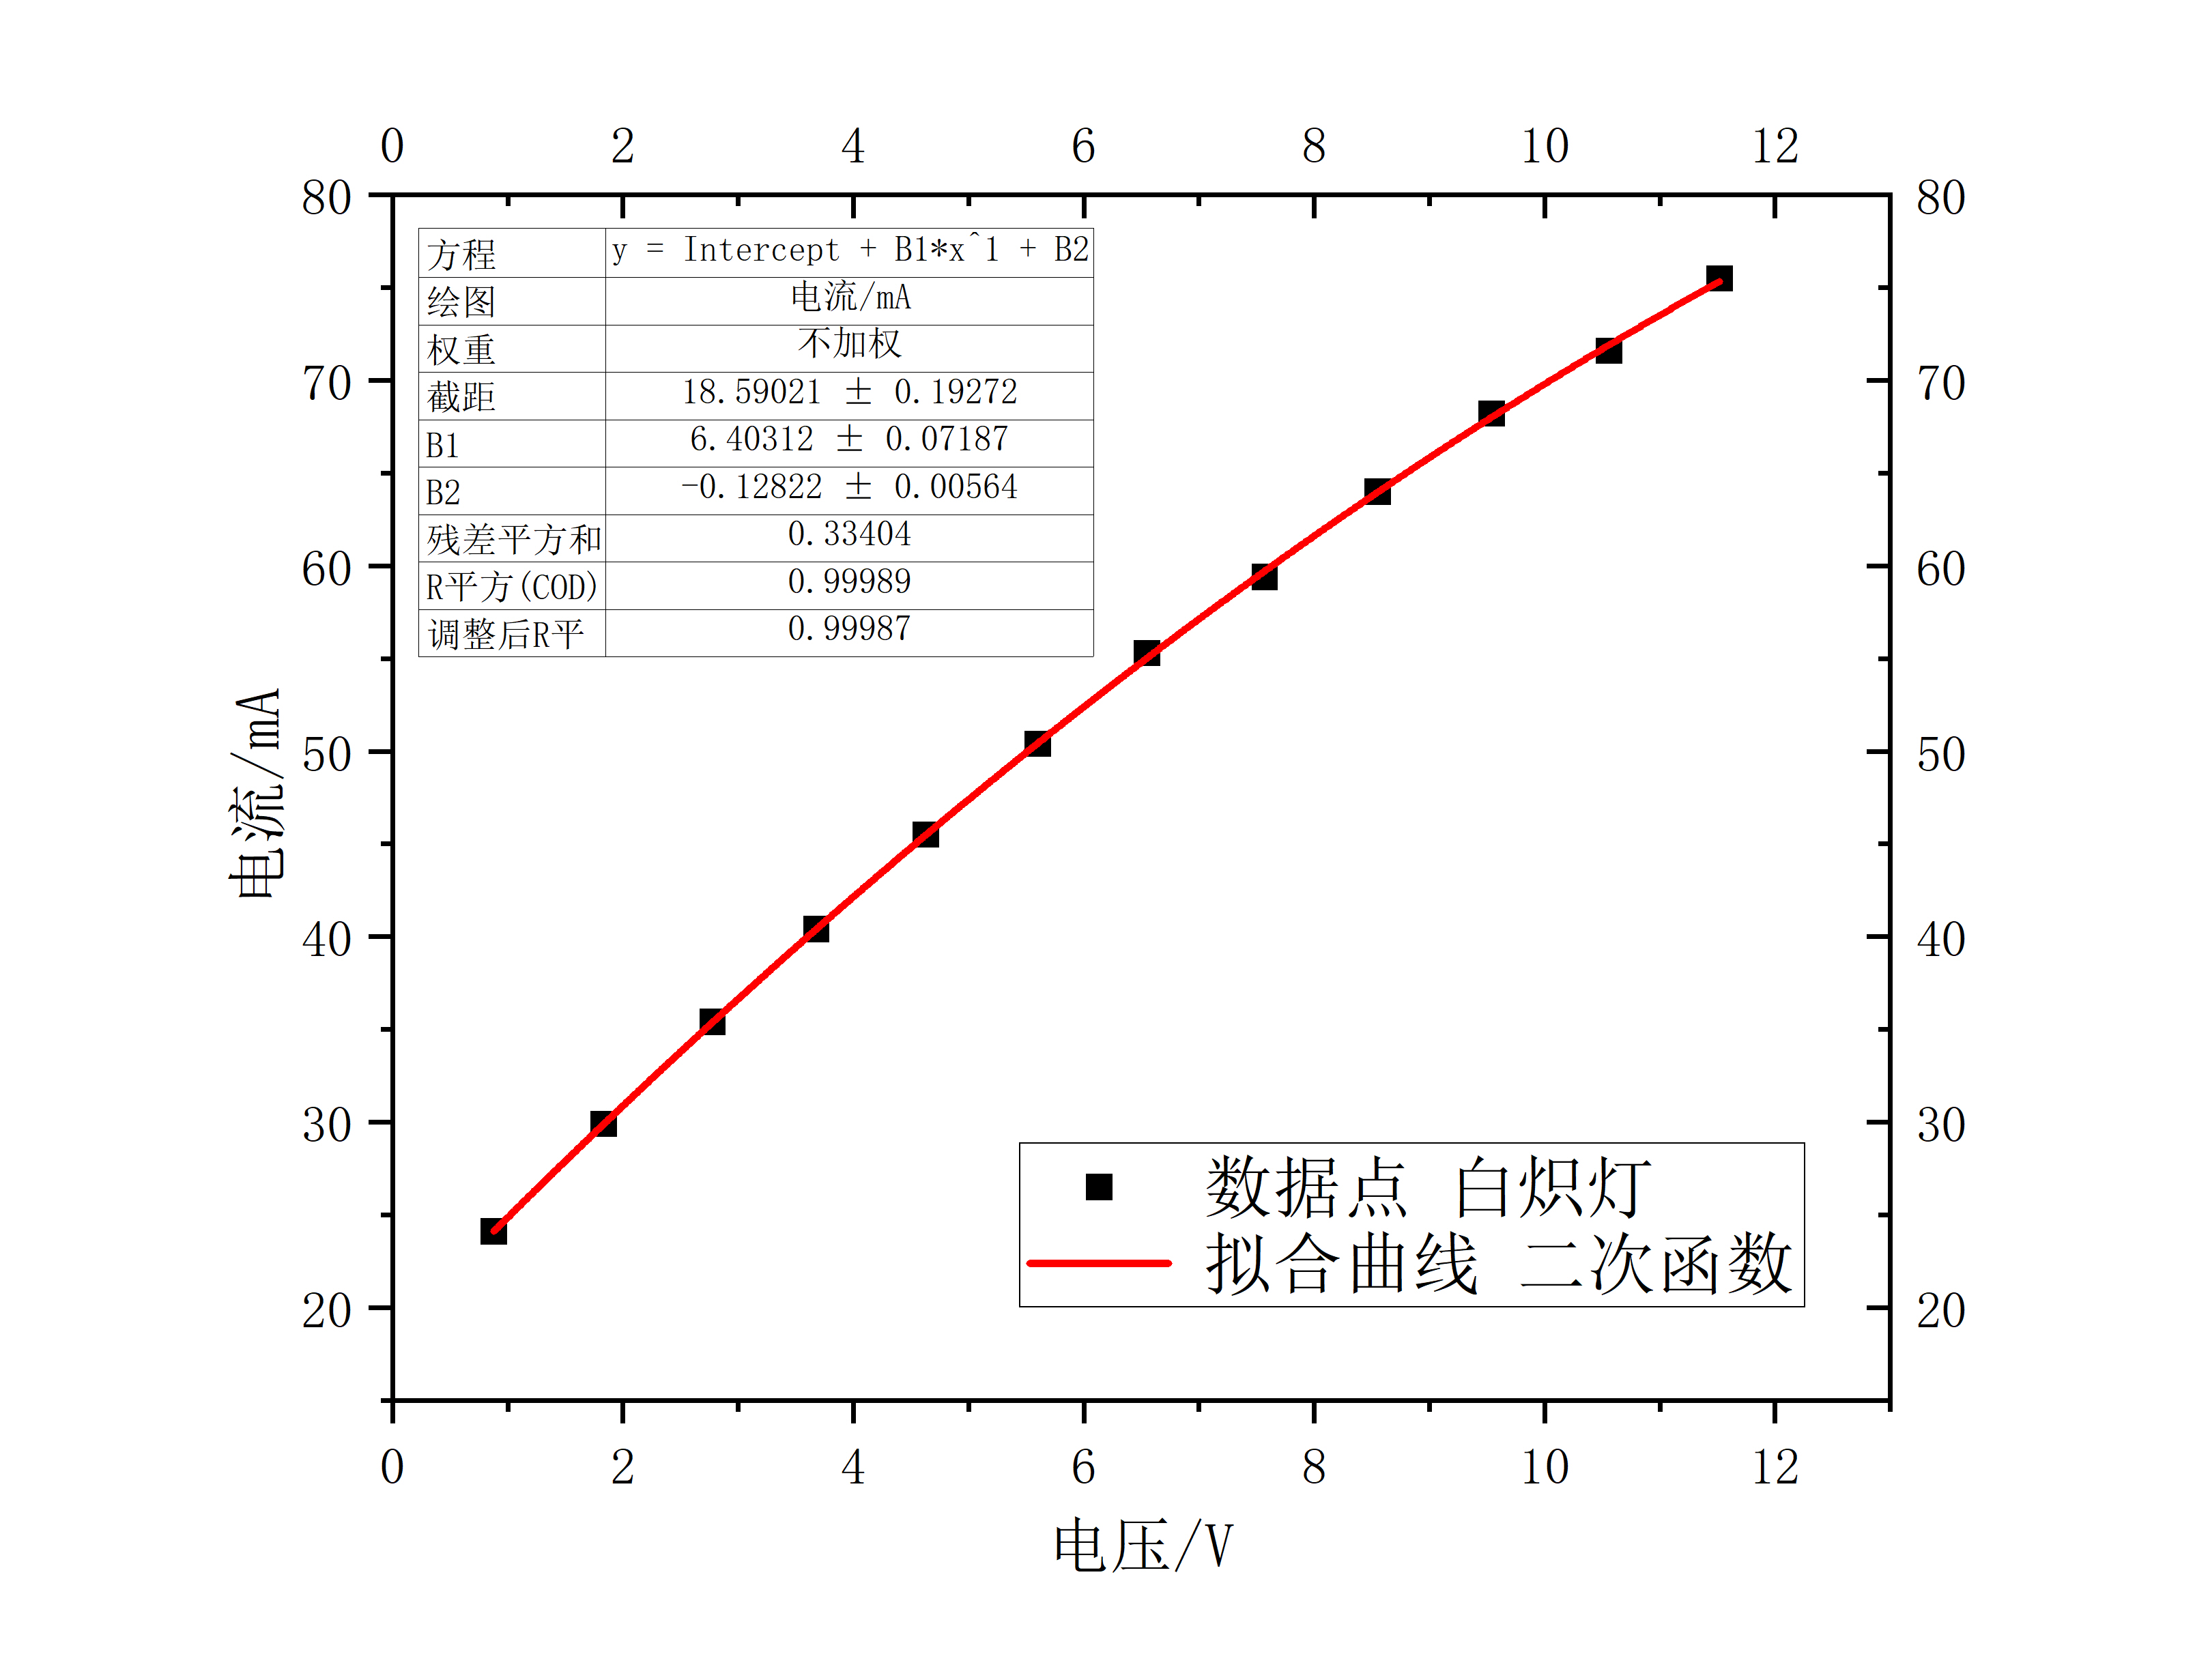
\includegraphics[width=0.7\textwidth]{ET1_2Gra7.jpg}
				\caption{12V 白炽灯伏安特性曲线}
				\label{fig:fig7}
			\end{figure}
			
			\item 白炽灯通常表现出非线性特性,这是因为它的电阻会随着温度的升高而增加,而温度的升高又是由通过灯丝的电流引起的。当电压增加时,流过灯丝的电流也增加,导致灯丝温度上升,进而导致电阻增加。这种电阻随温度变化的特性意味着电流随电压增加而增加的速率会逐渐减慢,形成一个非线性的伏安特性曲线。
			
			从二次方程中的系数 B2 可以看出,电流 I 关于电压 V 的二次项系数是负值($-0.12822 mA/V^2$),这意味着随着电压的增加,电流的增速会逐渐减慢。这与白炽灯电阻随温度增加而增加的特性相符合。
			
			R平方(COD)和调整后的R平方值仍然显示出模型与实验数据有很高的相关性,表明二次模型是合适的,可以很好地描述白炽灯的伏安特性。
		\end{enumerate}
				
		\item 测试直流稳压电源(DP832 或 DP831)CH2 的伏安特性
		\begin{enumerate}
			\item 根据实验所测得到的数据,直流稳压电源的伏安特性曲线作图如\cref{fig:fig8}所示。
			
			\begin{figure}[htbp]
				\centering
				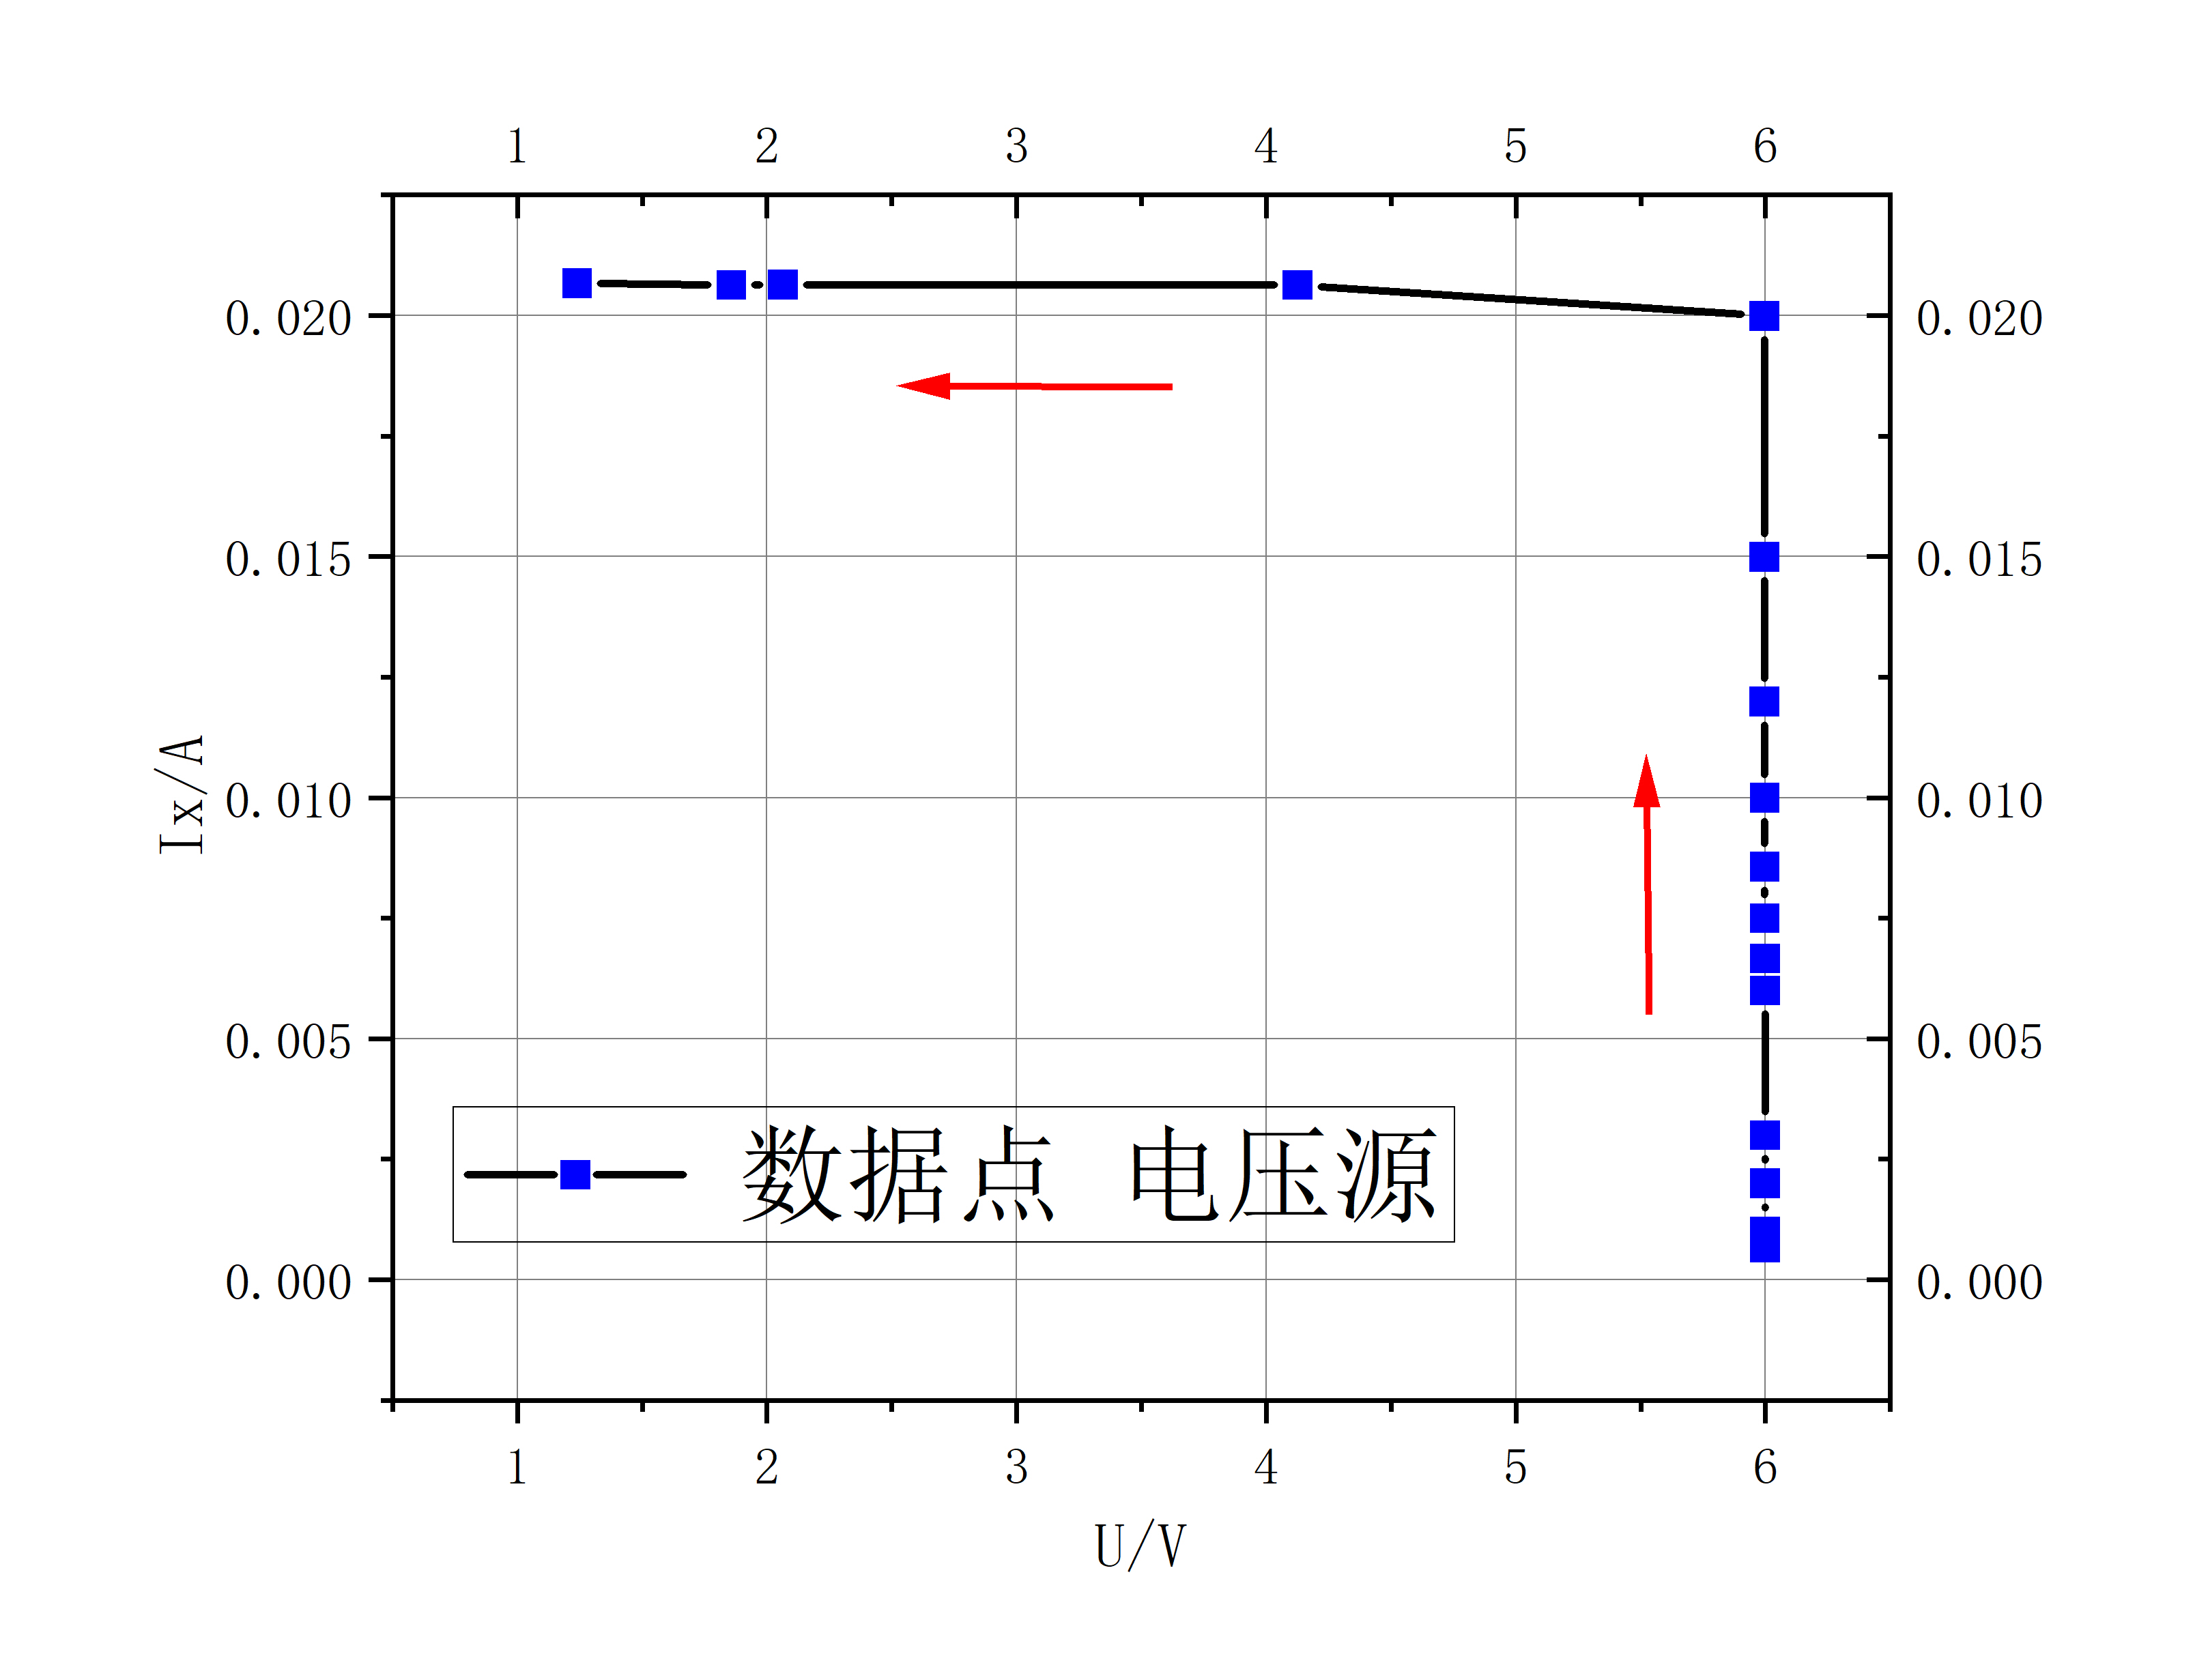
\includegraphics[width=0.7\textwidth]{ET1_2Gra8.jpg}
				\caption{直流稳压电源的伏安特性曲线}
				\label{fig:fig8}
			\end{figure}
			
			\item 达到阈值以前,他输出恒定的电压6V;达到阈值后,该元件变为一个恒流源。
		\end{enumerate}
				
		\item 测试数控恒流源(DCS-01)的伏安特性
		\begin{enumerate}
			\item 根据实验所测得到的数据,数控恒流源的伏安特性曲线作图如\cref{fig:fig9}所示。
			
			\begin{figure}[htbp]
				\centering
				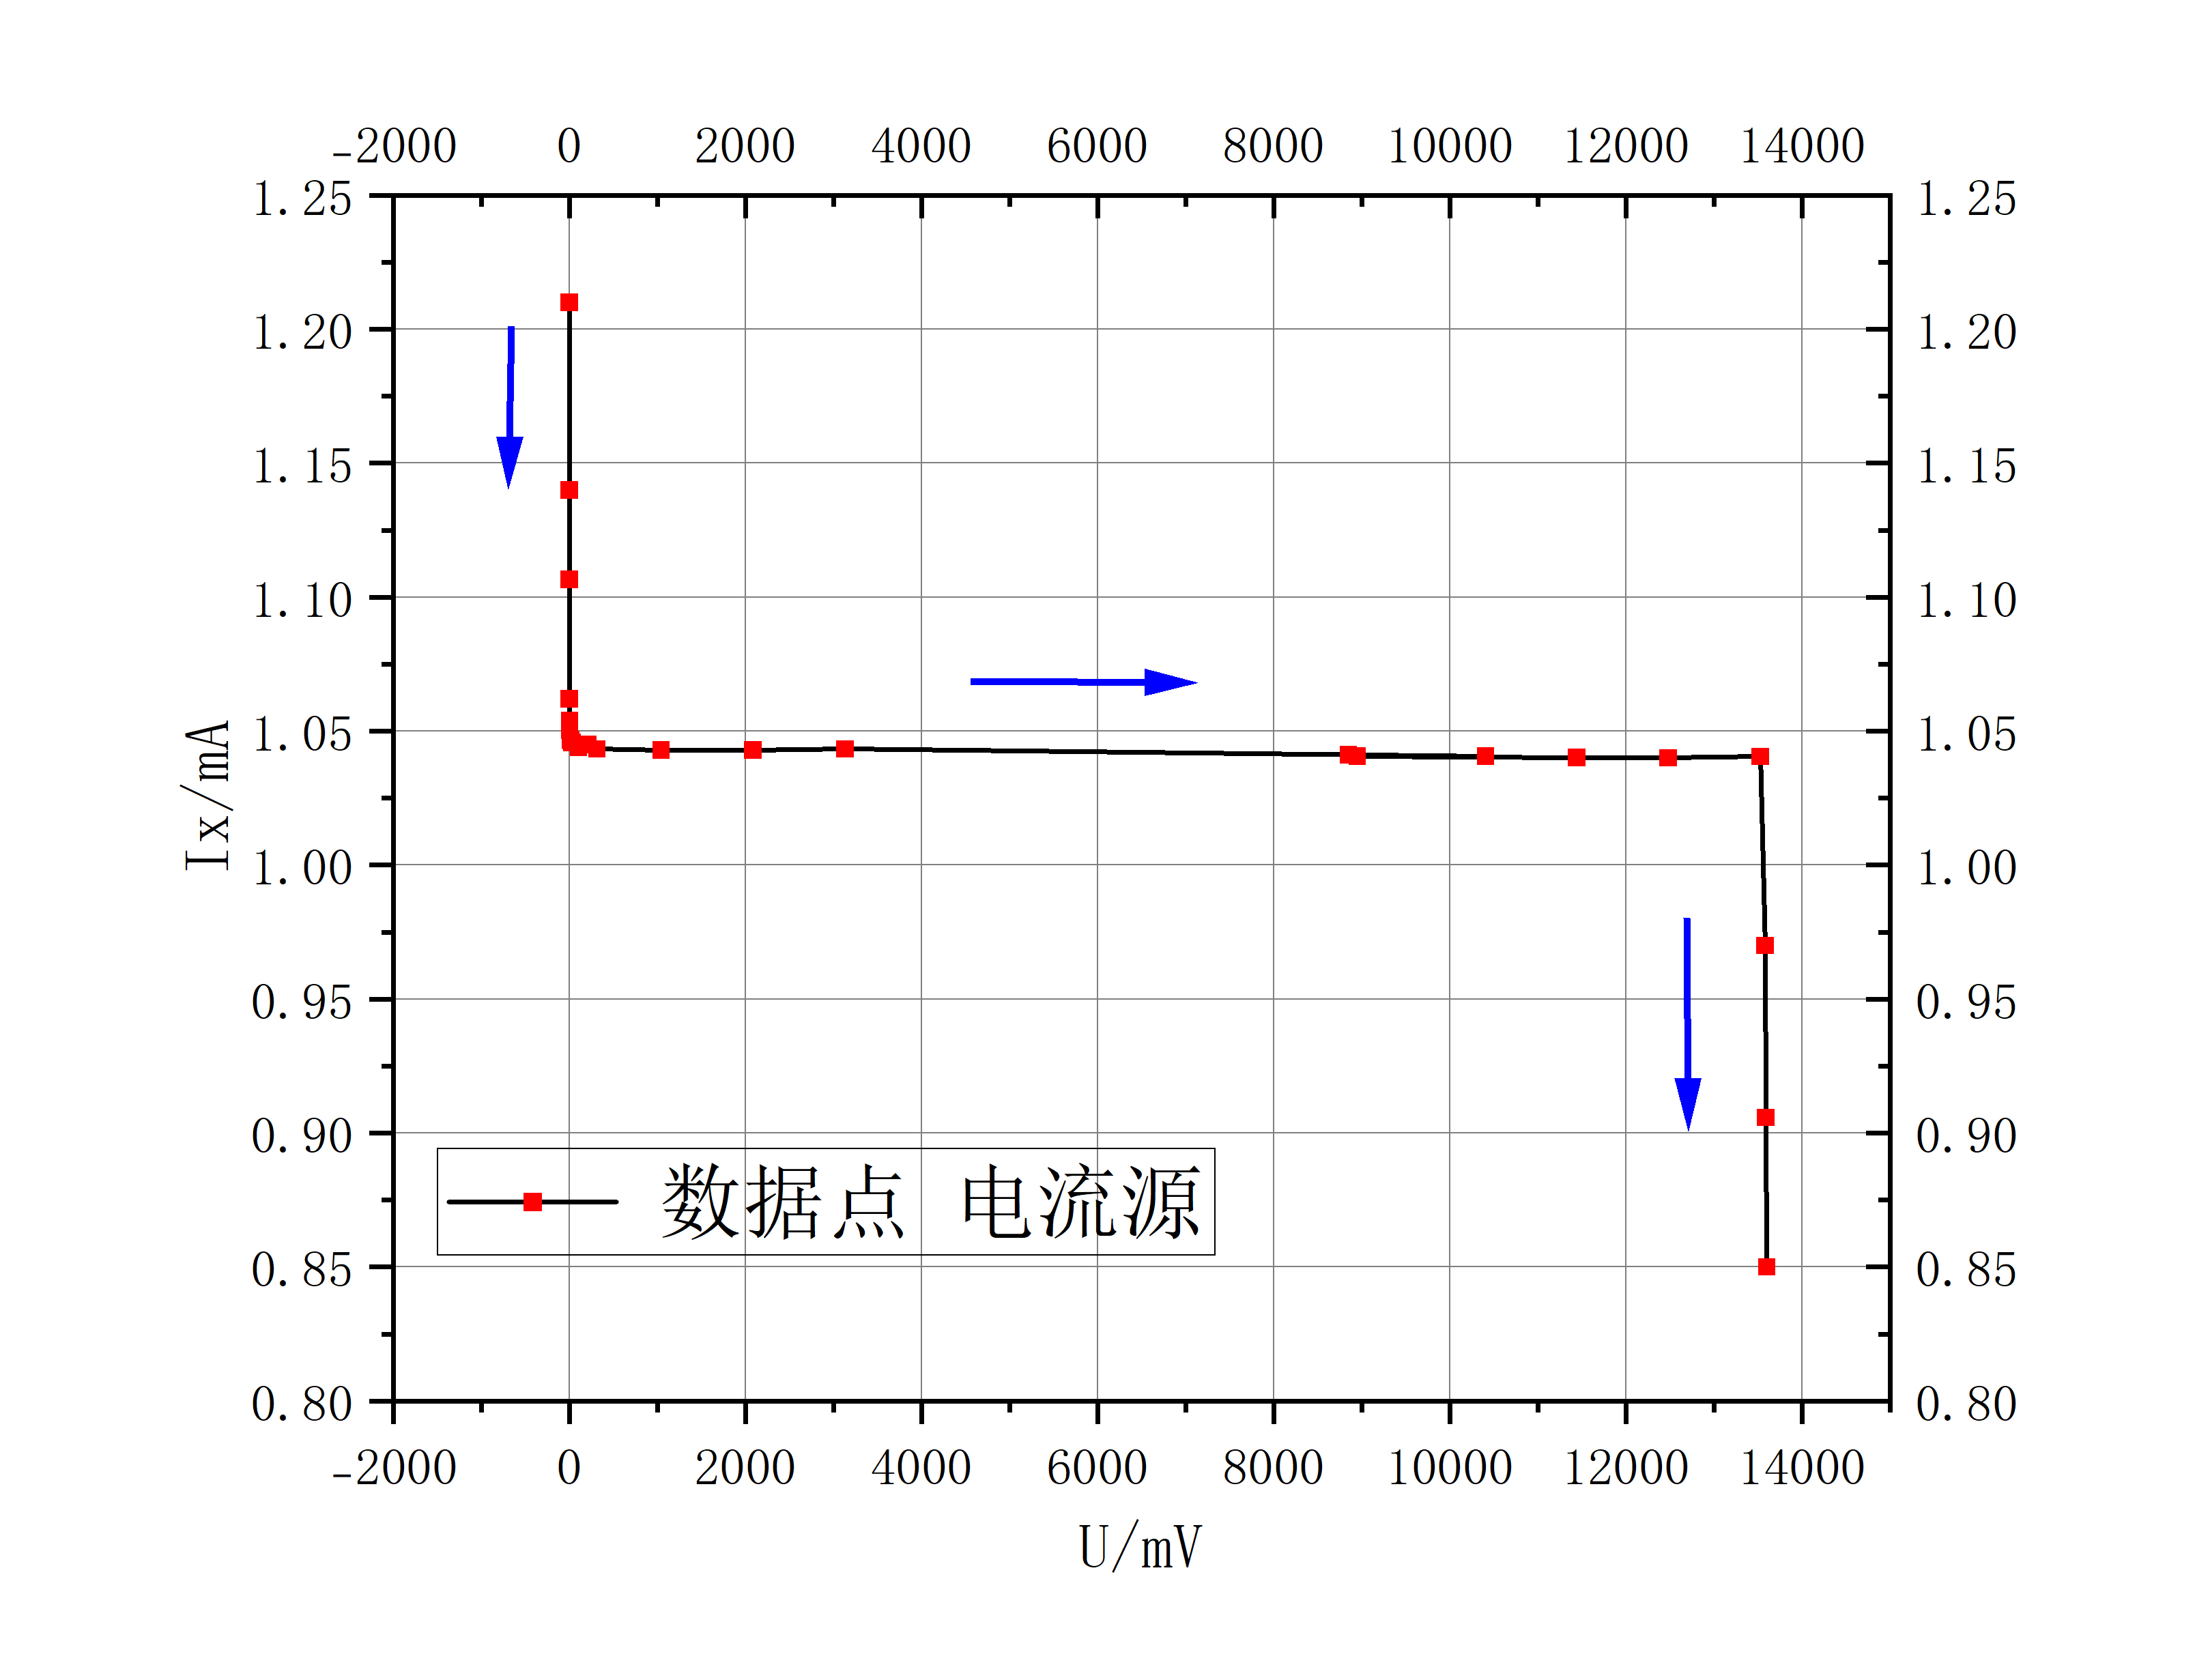
\includegraphics[width=0.7\textwidth]{ET1_2Gra9.jpg}
				\caption{数控恒流源的伏安特性曲线}
				\label{fig:fig9}
			\end{figure}
			
			\item 达到阈值前异常段分析:在0V附近的一段曲线,我们可以看到电流几乎不变,表现出恒压的特性。这可能是因为在电源两端的电压非常低时,恒流源内部的一些电子组件(如晶体管)尚未进入其正常工作状态,此时它们的行为类似于一个闭合的开关,导致电压在两端几乎没有变化,或者说电源维持了一个较低的,几乎恒定的电压值。在这个状态下,恒流源的输出特性更接近于一个恒压源。这种现象可能也与恒流源设计中的一些特定保护机制有关,例如,为了防止在低负载电压下过流,恒流源可能设计有一个最小电压下限,当电压低于这个下限时,会限制电流的增加。
			
			\item 达到阈值前:在大部分电压范围内,电流保持恒定,显示了恒流源的特性。但是,在两个端点,我们看到电流开始变化,表明电压超出了恒流源可以维持恒定电流的范围。
			
			\item 达到阈值后,该元件变为一个恒压源:曲线显示在大约13.7V的电压阈值处,电流迅速下降,
			表明恒流源不再能够维持设定的电流水平,电流开始受电压的限制。这种行为可能是由于恒流源的最大输出能力限制,或者是电源内部电路的过载保护特性。
		\end{enumerate}
		
	\end{enumerate}
	
	%
	\subsubsection{关于外接法与内接法的数据分析}
	\begin{enumerate}
		\item 外接法内接法的误差理论分析
		
		\begin{figure}[htbp]
			\centering
			\subfloat[]{
				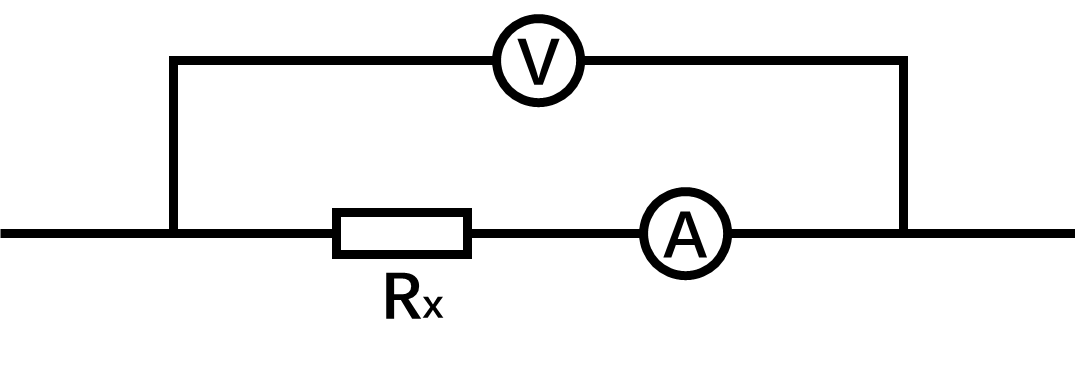
\includegraphics[width=0.4\textwidth]{ET1_2GraVA1.png}
			}
			\subfloat[]{
				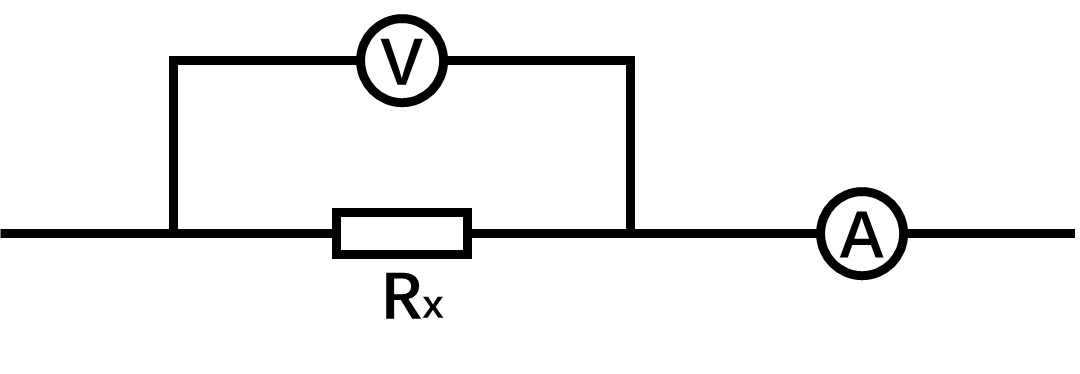
\includegraphics[width=0.4\textwidth]{ET1_2GraVA2.png}
			}
			\caption{分别是内接法和外接法}
			\label{fig:figVA1}			
		\end{figure}
		
		如图所示,根据外接法和内接法的电路图,我们可以从理论上分析出外接法和内接法的误差,并据此选择采用哪一种方式。
		
		\begin{figure}[htbp]
			\centering
			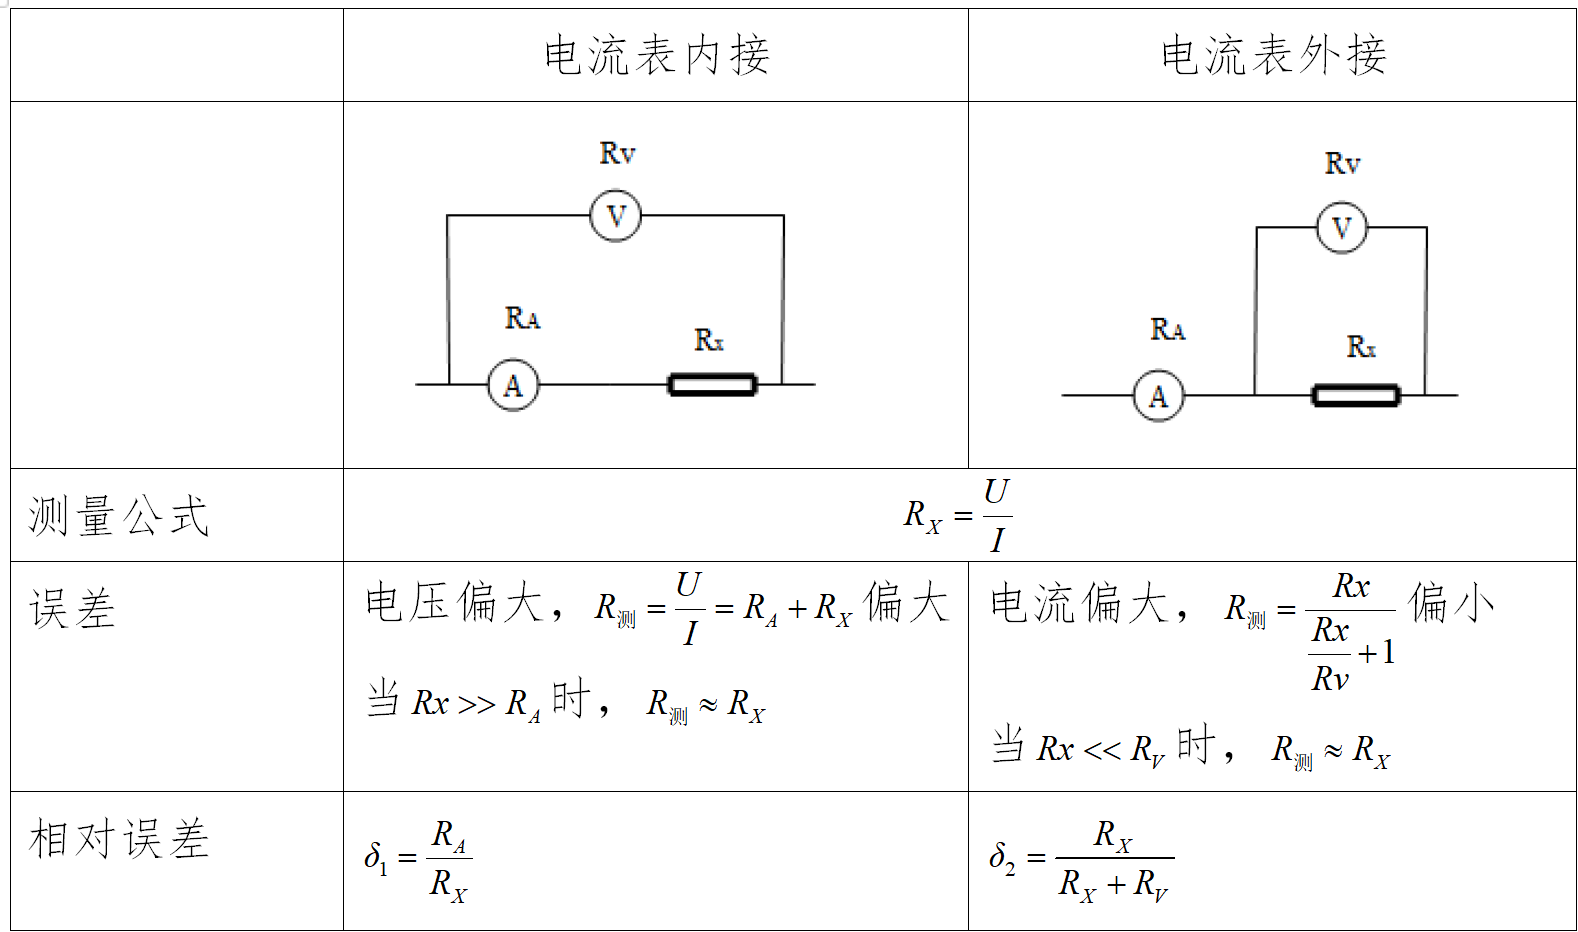
\includegraphics[width=0.8\textwidth]{ET1_2GraVA3.png}
			\caption{外接法和内接法误差分析}
			\label{fig:figVA}
		\end{figure}

		当 $\delta_1 < \delta_2$ 时,使用内接法相对误差较小,即 $\frac{R_A}{R_x} < \frac{R_x}{R_x + R_{V}} \Rightarrow R_A \cdot (R_x + R_{V}) < R^2_x$。因为电流表内阻很小,忽略 $R_A$,有 $R_A R_V < R^2_x \Rightarrow R_x > \sqrt{R_A R_{V}}$。同理可证其他情况。

		
		\item 本实验实测外接法和内接法的误差分析
		
		本实验使用外接法和内接法测定结果如图所示,根据测量结果,得到的误差情况如表所示。
		
		\begin{table}[h]
			\centering
			\caption{线性元件外接内接误差}
			\label{tab:tab6}
			\begin{tabular}{|c|c|c|c|c|c|c|c|}
				\hline
				\multicolumn{2}{|c|}{51Ω 外接} & \multicolumn{2}{c|}{51Ω 内接} & \multicolumn{2}{c|}{120Ω 外接} & \multicolumn{2}{c|}{120Ω 内接} \\
				\hline
				实验 & 理论 & 实验 & 理论 & 实验 & 理论 & 实验 & 理论 \\
				\hline
				50.41 & 51 & 51.56 & 51 & 117.97 & 120 & 119.36 & 120 \\
				\hline
				相对误差 & -1.16\% & 相对误差 & 1.10\% & 相对误差 & -1.69\% & 相对误差 & -0.53\% \\
				\hline
			\end{tabular}
		\end{table}
		
		\textbf{51Ω 电阻}
		
		\begin{itemize}
			\item \textbf{外接法(串联法)}
			\begin{itemize}
				\item 实验值:50.41Ω
				\item 理论值:51Ω
				\item 相对误差:-1.16\%
			\end{itemize}
			
			这里的负误差表明实际测量值比理论值略小。在外接法中,电流表内阻可能会导致测得的电压值偏小,从而导致计算出的电阻值偏小。
			
			\item \textbf{内接法(并联法)}
			\begin{itemize}
				\item 实验值:51.56Ω
				\item 理论值:51Ω
				\item 相对误差:1.10\%
			\end{itemize}
			
			这里的正误差表明实际测量值比理论值略大。在内接法中,电压表的内阻会导致测量电流时部分电流通过电压表,从而减少了通过未知电阻的电流,这可能导致测量出的电阻值偏大。
		\end{itemize}
		
		\textbf{120Ω 电阻}
		
		\begin{itemize}
			\item \textbf{外接法(串联法)}
			\begin{itemize}
				\item 实验值:117.97Ω
				\item 理论值:120Ω
				\item 相对误差:-1.69\%
			\end{itemize}
			
			对于较大的电阻值,电流表的内阻对总电阻的影响比较小,但仍旧可能造成一定的测量误差,导致实际测量值略低于理论值。
			
			\item \textbf{内接法(并联法)}
			\begin{itemize}
				\item 实验值:119.36Ω
				\item 理论值:120Ω
				\item 相对误差:-0.53\%
			\end{itemize}
			
			在内接法中,由于电压表的内阻一般很大,对于较高的电阻值,电压表的影响很小,因此测量误差也较小。这里的实际测量值接近理论值,误差很小。
		\end{itemize}
		
	\end{enumerate}
	
	
	%
	\subsubsection{受控源CCVS的特性分析}
	这一小节将对所测得的CCVS的转移特性与输出特性做分析。
	\begin{enumerate}
		\item 根据实验所测得的数据(\cref{tab:tabA1}和\cref{tab:tabA2}),绘图如\cref{fig:figA1}所示。
		
		\begin{figure}[htbp]
			\centering
			\subfloat[]{
				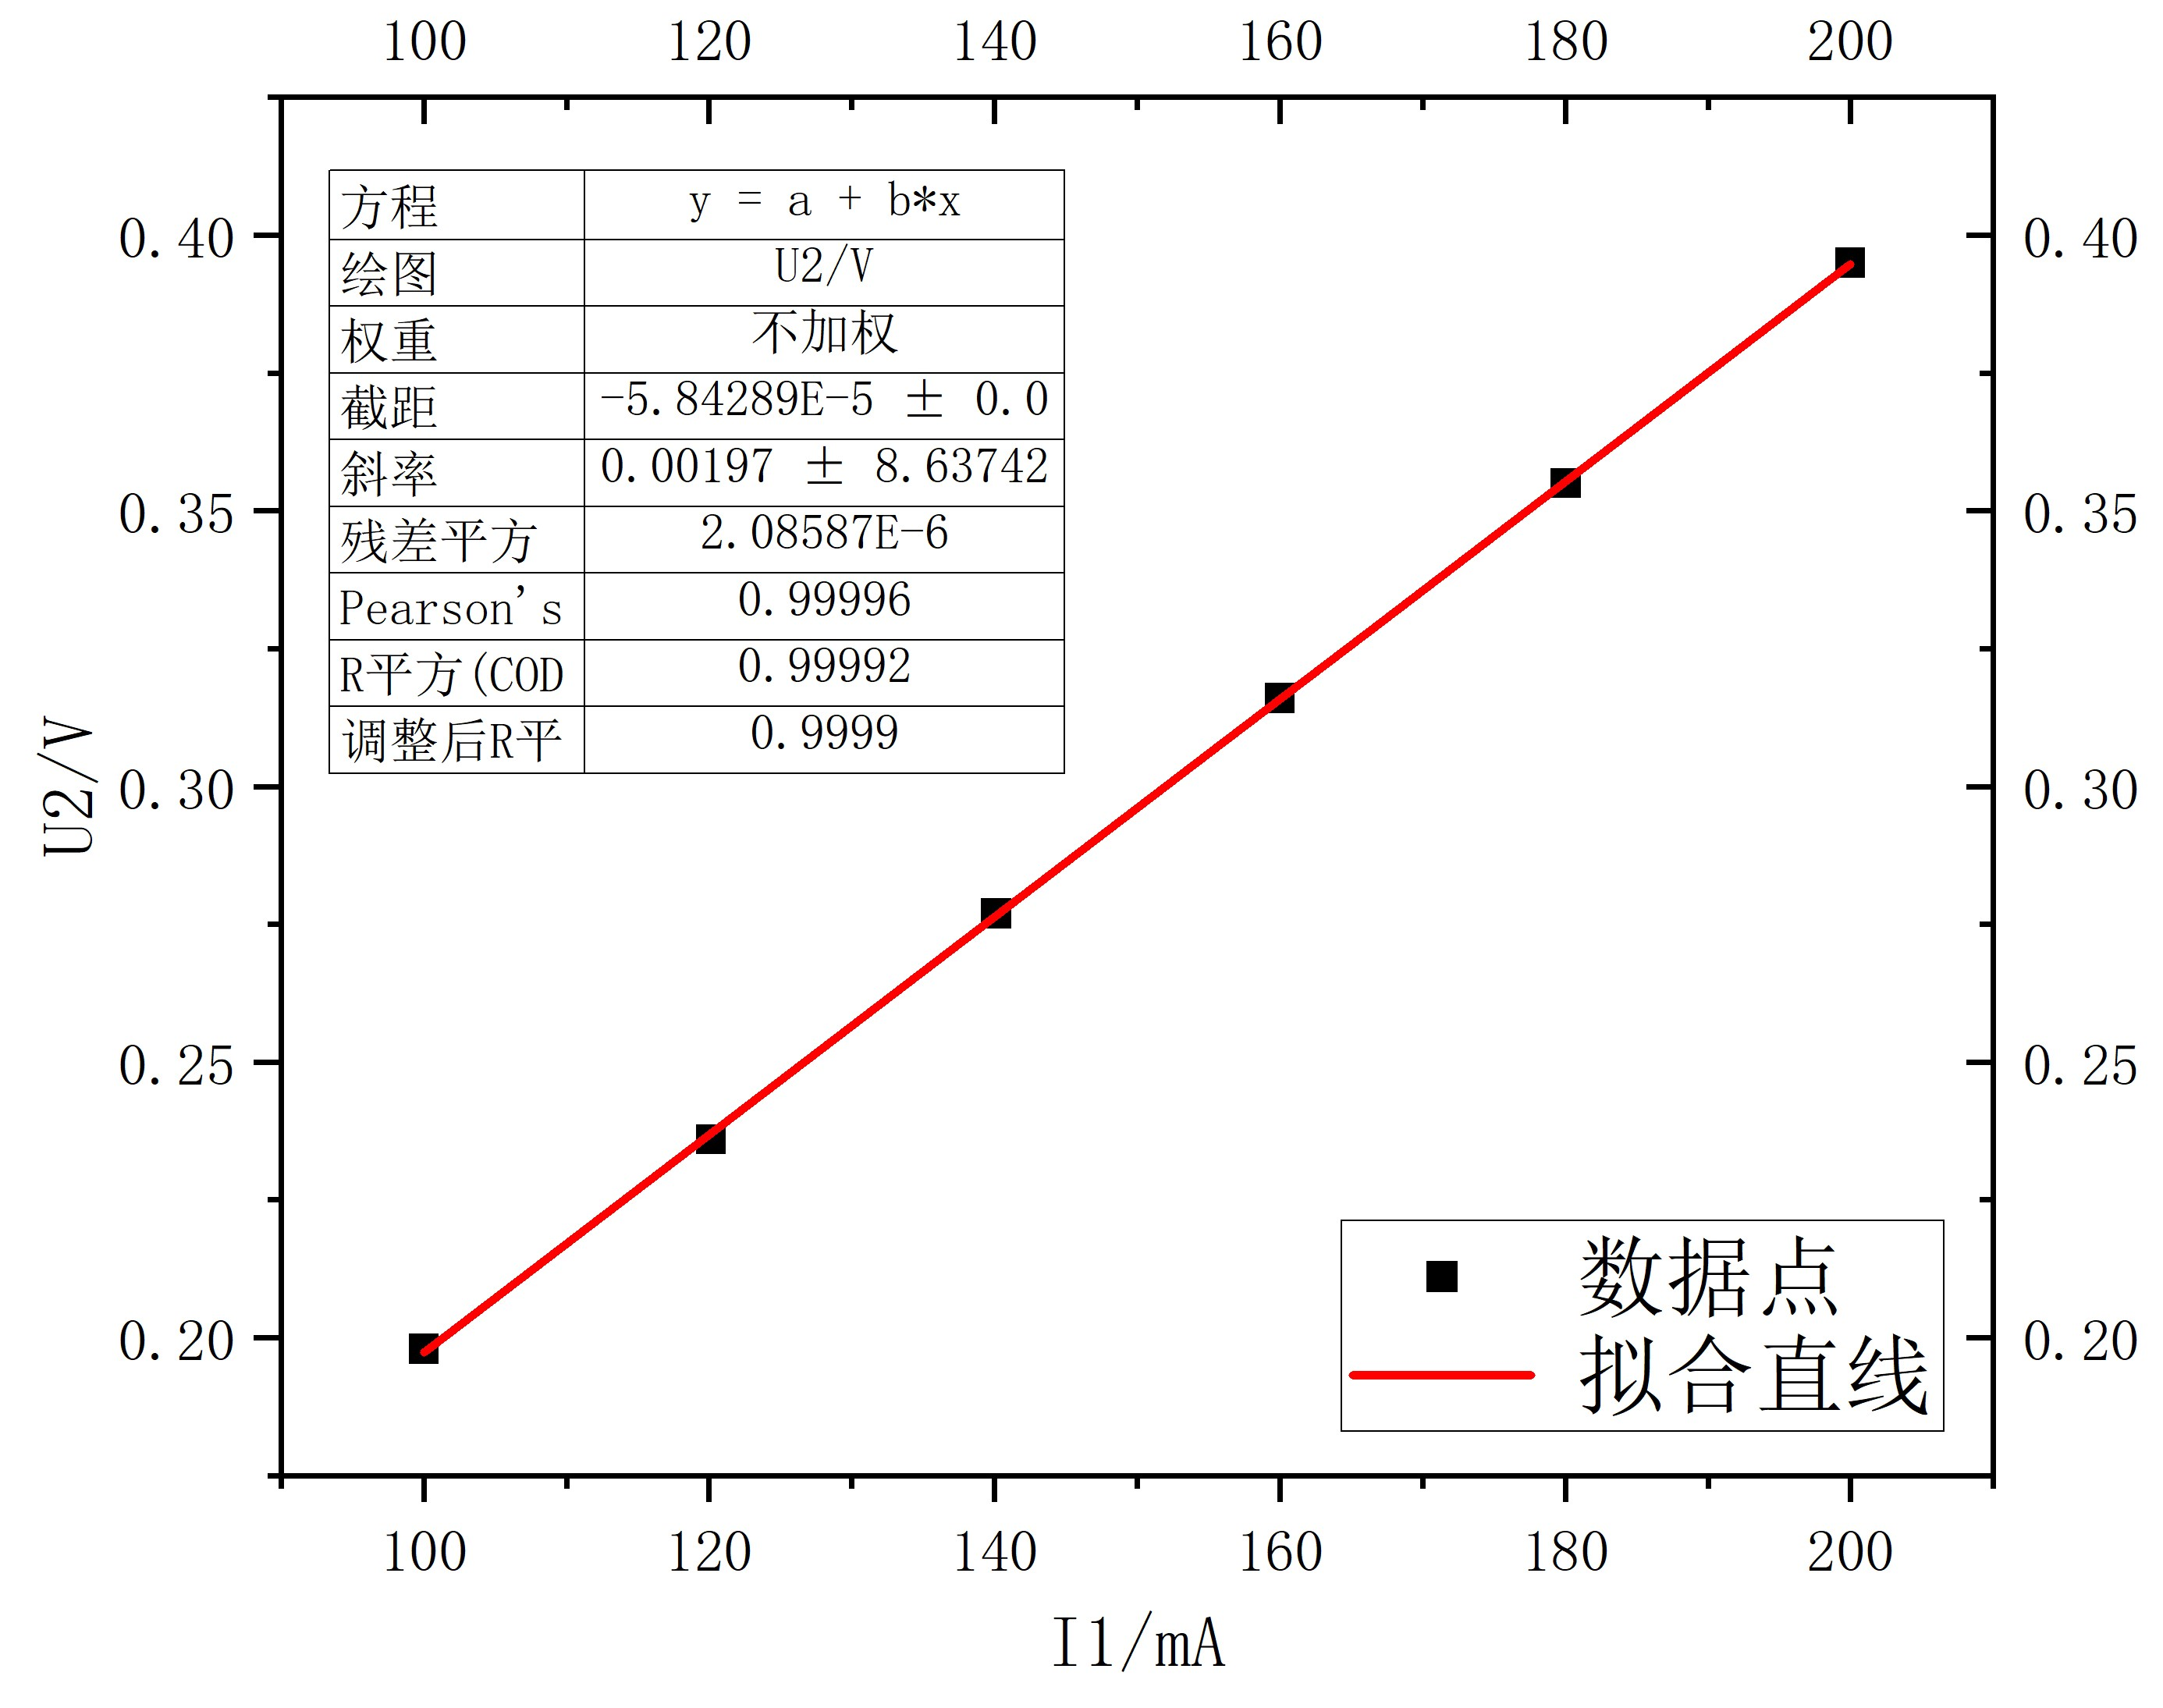
\includegraphics[width=0.45\textwidth]{ET1_2GraA1.jpg}
			}
			\subfloat[]{
				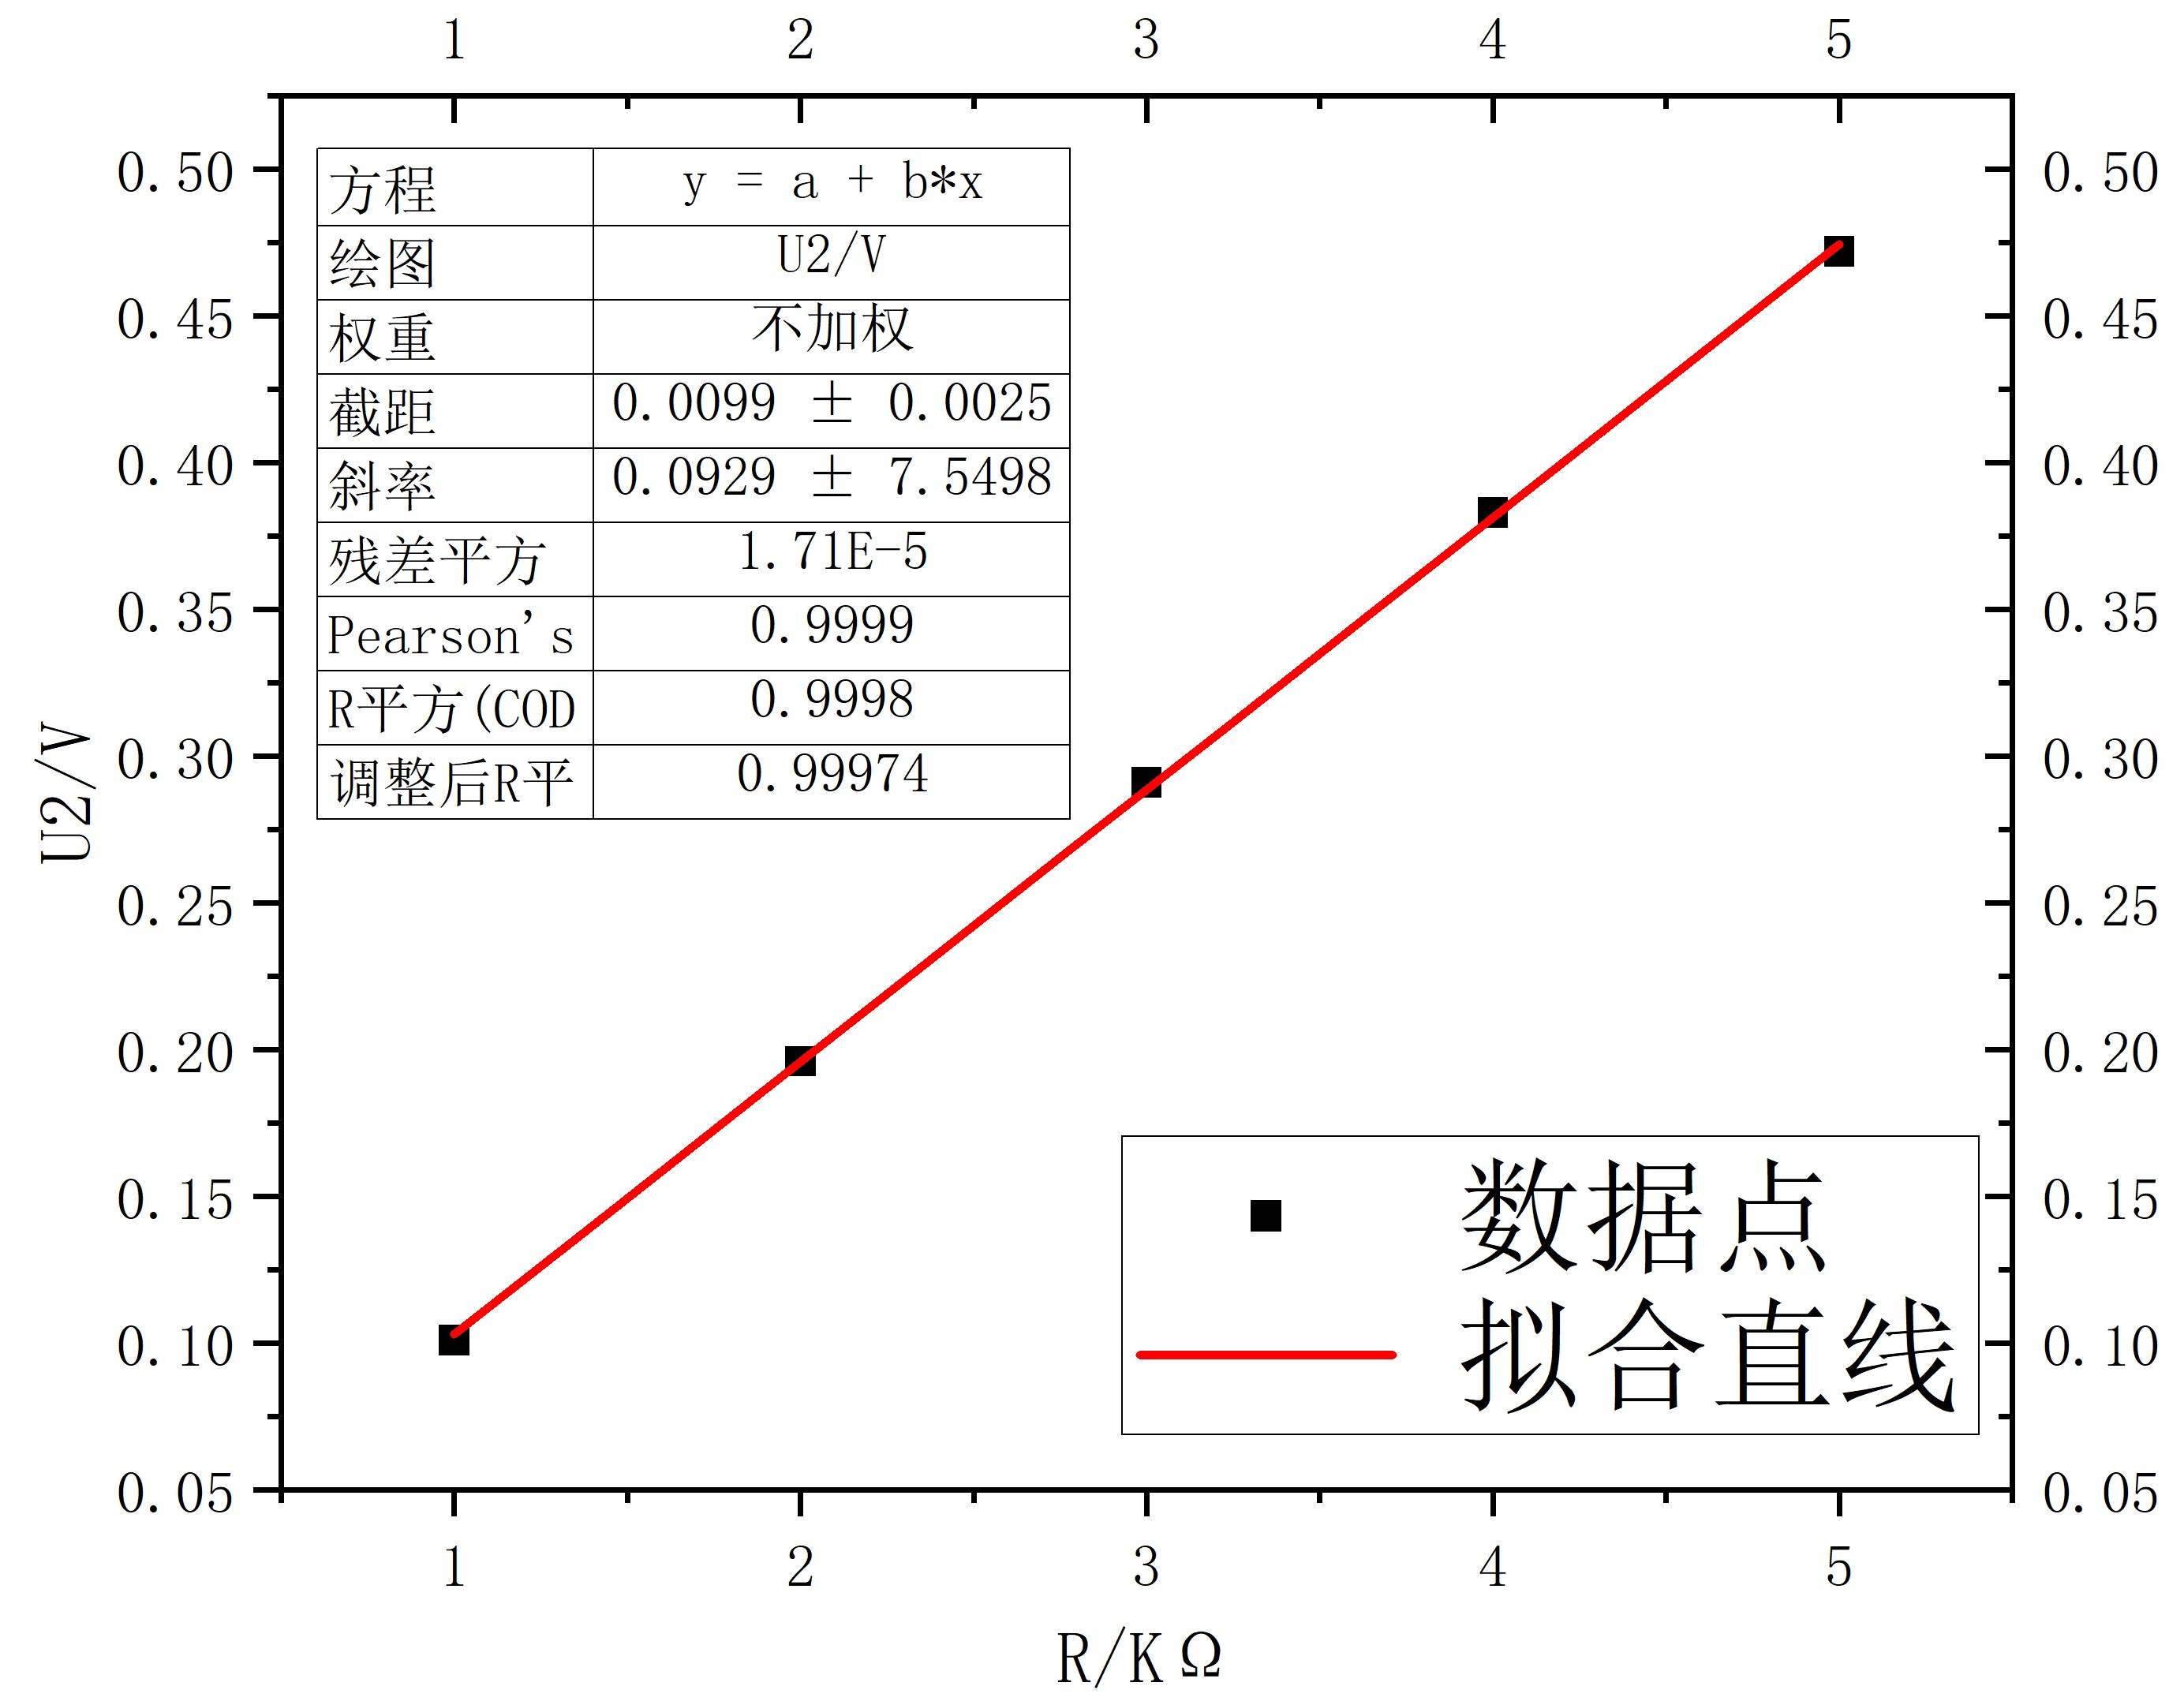
\includegraphics[width=0.45\textwidth]{ET1_2GraA2.jpg}
			}
			\caption{a:转移特性;b:输出特性}
			\label{fig:figA1}			
		\end{figure}
		
		\item 从转移特性曲线我们可以看出,它有着良好的线性关系,相关系数相对接近1;即在负载电阻阻值恒定的情况下,输出电压U2确实受控制电流I1控制。
		
		\item 注意到我这里作的输出特性的图是负载电阻R与输出电压U2间的关系。理论上来讲,在控制电流I1不变的情形下,U2也应当不变才对。然而事实上U2变化了,还与R有着良好的线性关系,相关系数接近1。进一步测量发现,I2反而是几乎不变的,因此这说明这个“CCVS”在事实上是一个CCCS,即应当是输出电流I2受控制电流I1控制。
		
	\end{enumerate}
	
	%
	%\subsubsection{其它问题的分析与讨论}
	
	% ---
	
	% 实验后思考题
%	\subsection{实验后思考题}
	
	% ---
	
	
	% 结语部分
	\clearpage
	
	% 小标题
	\section{实验二\quad 基本电路元件伏安特性的测量 \quad\heiti 结语}
	% ---
	
	% 总结、杂谈与致谢
	\subsection{实验心得和体会、意见建议等}
	\begin{enumerate}
		\item 实验心得体会
			\begin{enumerate}
				\item 理论与实践的结合:通过这次实验,我对电路理论有了更深刻的理解。实际操作中,我能够将抽象的理论知识应用到具体的电路设计中,这让我认识到了学习理论知识的重要性。
				
				\item 技术技能的提高:在实验过程中,我对电路的搭建和测量技术变得更加熟练。特别是在使用测量工具时,我学会了如何更精确地获取和分析数据。
				
			\end{enumerate}
		
		\item 意见和建议
			\begin{enumerate}
				\item 完善实验指导:希望能够对实验指导书进行更新,使其内容更加详尽,尤其是在描述实验步骤时。同时,对于可能遇到的问题,提供更多的提示和解决策略。
				
				\item 设备的定期维护:建议定期对实验室设备进行维护和升级,以避免实验中出现设备故障,影响实验进度和结果。这次的实验中测量“受控源CCVS的特性分析”时,就出现了偏离实验预期的结果,测出来实际是CCCS,在实验中耽误了一定的时间。
				

			\end{enumerate}
			
		\item 感谢老师能阅读这篇还有很多不足的实验报告,希望老师能指出做得不好的地方;祝老师身体健康、生活幸福、工作顺利!
	\end{enumerate}
	% ---
	
	% 参考文献
	\subsection{参考文献}
	[1] 维基百科 https://zh.wikipedia.org
	
	[2] 电子技术实验 保延翔 2020.07 中山大学公共实验教学中心
	
	% ---
	
	% 附件
	\subsection{附件及实验相关的软硬件资料等}
	试验台桌面整理如\cref{fig:table}所示。

	\begin{figure}[htbp]
		\centering
		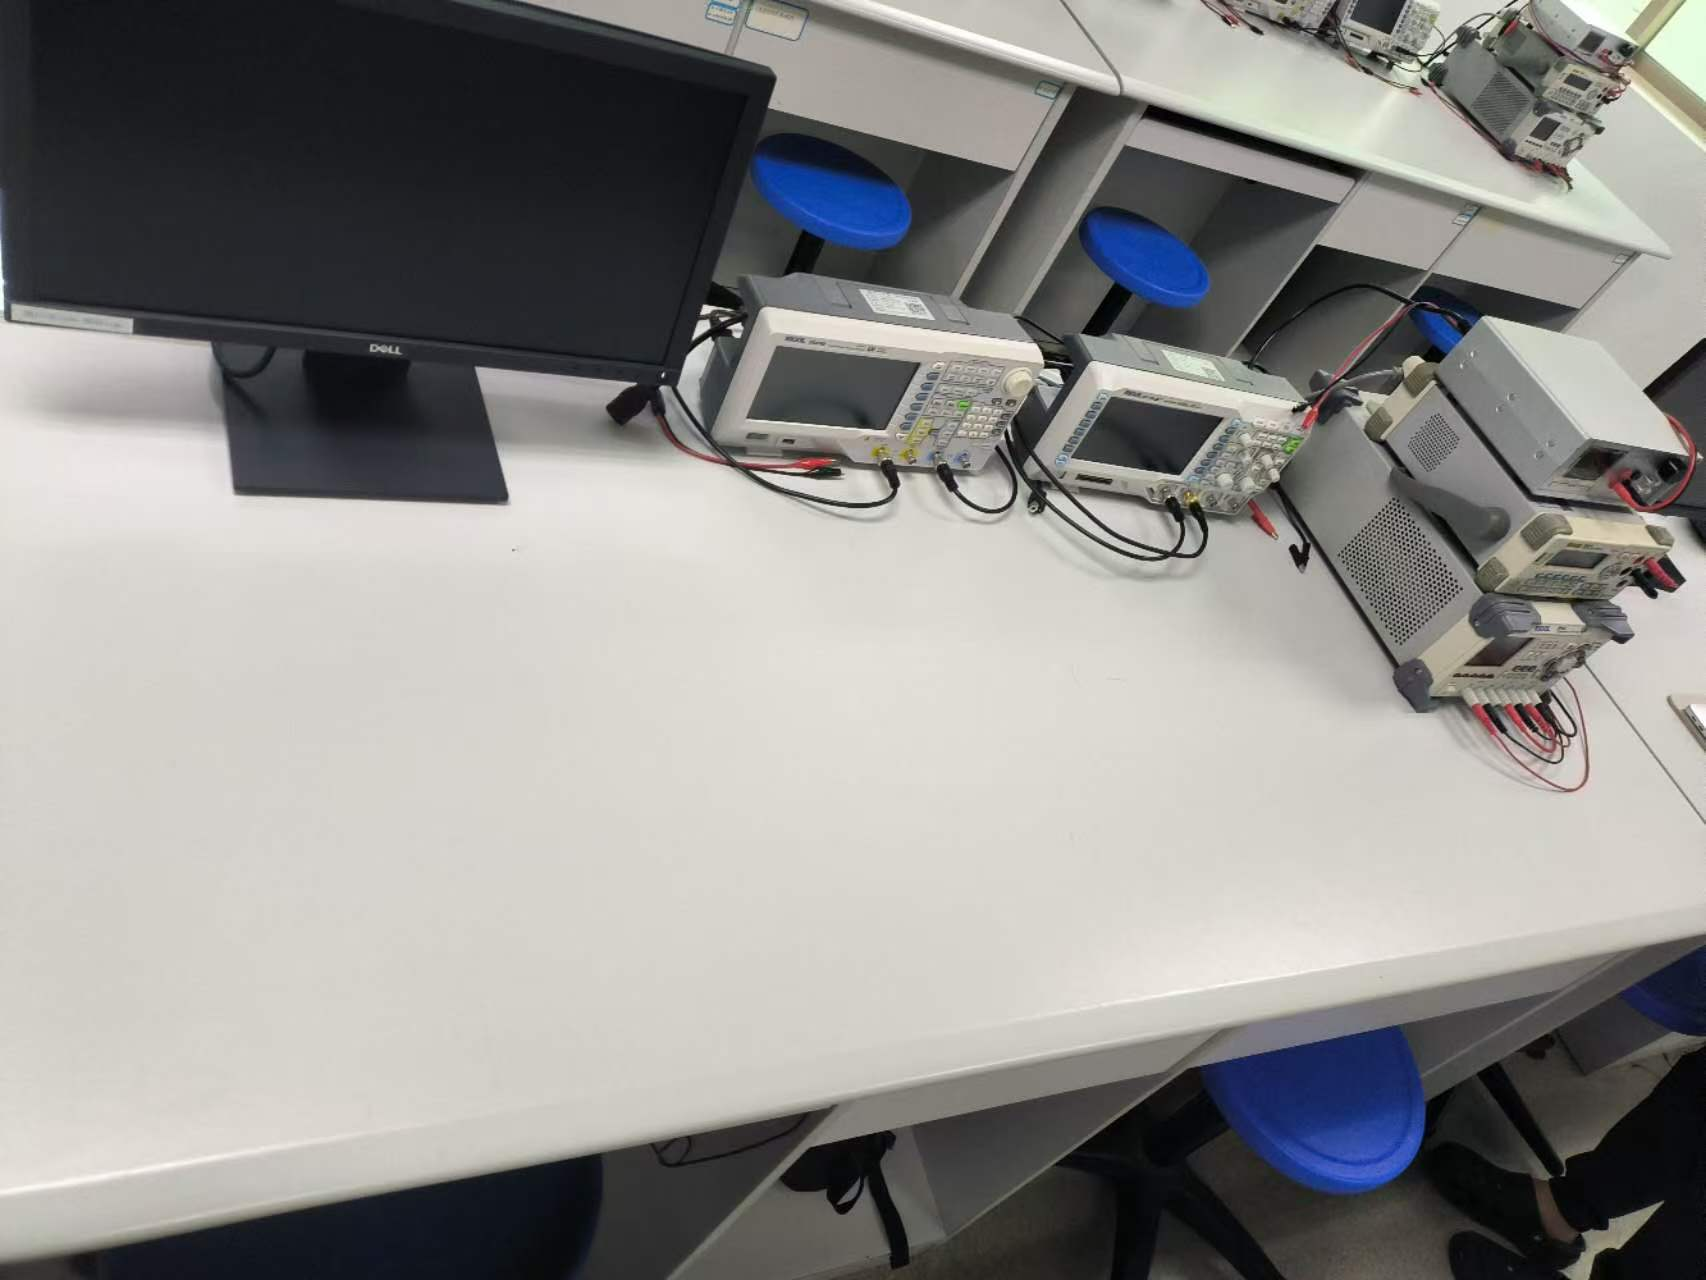
\includegraphics[width=0.5\textwidth]{table.jpg}
		\caption{试验台桌面整理}
		\label{fig:table}
	\end{figure}
	
	实验报告个人签名如\cref{fig:name}。
	
	\begin{figure}[htbp]
		\centering
		\subfloat[]{
			
\includegraphics[width=0.45\textwidth]{name.png}
		}
		\subfloat[]{
			
\includegraphics[width=0.45\textwidth]{name-TaLEs.jpg}
		}
		\caption{个人签名}
		\label{fig:name}			
	\end{figure}

	% \begin{figure}[htbp]
	% 	\centering
	% 	
\includegraphics[width=0.7\textwidth]{name.png}
	% 	\caption{个人签名}
	% 	\label{fig:name}
	% \end{figure}
	
	% ---
	
	相关代码已上传至Github。
	
	
	
\end{document}